% Chapter 3

% variables
\newcommand{\pdirthree}{chapters/plots/chapter3}

\chapter{Data analysis}
\label{chapter3}

% ----------------------------------------------------------------------------------------

In the previous chapter, we explored the general concepts and the main characteristics of the invisible and visible mode setup. In this one, we will describe the method used to analyze them. In Sec.\ref{ch3:sec:analysis-approach}, the analysis performed will be detailed step by step. I contributed heavily to the development of a reconstruction software for the data collected, with a focus on the MM information and the reconstruction of the track's momentum. I also wrote the software to reconstruct data from Straw Tube together with Peter Degen \cite{pdegen-thesis}, a master student I supervised in our group. After that, a description of the simulation framework will be provided in Sec.\ref{ch3:sec:geant4}, which is the main tool used to compute both background and signal rate. I was one of the main contributors to this software, and I participate heavily in the testing of all its functionalities. In particular, I took care of the detailed implementation of MM and GEM, and I wrote a procedure to transform the simulation output in a format equivalent to the one used for the data, which is detailed in Sec.\ref{ch3:sec:geant4-digitization}. A correction to the hadron model used in the simulation to improve the MC-data agreement was also part of my work, detailed in Appendix.\ref{appC:sec:ftfp-modifications}.
In Sec.\ref{ch3:sec:dimuons}, we will show how the rare interaction $\emu$ is used in NA64 as an important tool to validate the MC and correct the signal yield for systematic effects.
A detailed description of two background rejection techniques developed as direct consequence of my work, namely SRD rejection and shower profile analysis, will be given in Sec.\ref{ch3:sec:bkg-srd}-\ref{ch3:sec:bkg-ecal-profile}.
Finally, a description is provided of both visible and invisible mode analyses in Sec.\ref{ch3:sec:analysis-invis} and Sec.\ref{ch3:sec:analysis-vis} respectively. In the case of the visible mode, this section also includes the new visible analysis based on trackers information which I performed during my thesis. To complete this analysis, I also wrote code to reconstruct more precisely tracks and vertices in the decay volume, now part of the main reconstruction software used by NA64.
A list of selection criteria and background sources is provided for each analysis. We show that in both modes the background is under control, with an expected number of events in the signal box of $\simeq 0.5$ for the invisible mode and $\simeq 0.01$ for the visible one.


\section{General Analysis approach}
\label{ch3:sec:analysis-approach}

To shape the analysis the choice of the signal region and the selection criteria are crucial, which means deciding what are the characteristics that define a candidate $\DM$ event.
The figure of merit is to maximize the sensitivity of the experiment. In other words, if $\DM$ does exist, the analysis should maximize its discovery probability, and minimize the probability of producing a false positive. In this type of experiments, the number of events in the signal region is counted and compared to the expected background calculated. Assuming, that the number of events in the signal region follows a Poisson distribution, we can express the number of expected events in the signal region $N_{SR}$ using:
\begin{equation}
  \label{eq:poisson-simple}
  N_{SR} = \frac{(\mu s + b)^ne^{-(\mu s + b)}}{n!}
\end{equation}
where $s$ and $b$ represent the expected number of events for signal and background in the signal region, and $\mu$ is a control parameter that describes if the signal is present. If it is properly modeled, the parameter $\mu$ can be either 0 (no signal present) or 1 (signal is there), but we can also choose to allow a continuous spectrum of $\mu$, which means that the signal can have a larger (or smaller) rate. The experiment will claim a signal if the number of events exceeds significantly the expected background $b$, such that $\mu = 0$ is no longer compatible with the data. The most common standard for discovery in the HEP\footnote{High Energy Physics.} community is the 5$\sigma$ criteria. This means that the number of events is larger than the one predicted by the $\mu = 0$ hypothesis by 5 standard deviations\footnote{This is to be intended as the correspondent p-value in a Gaussian distribution. The actual distribution defining the number of events expected is typically computed using numerical methods.}. The probability of an experiment returning such an outcome when no signal exists is 2.87$\times$10$^{-7}$.

If no signal is observed, a second problem arises, how do we interpret this result? In principle, since the initial no-signal hypothesis (frequently called $H_0$) is sufficient to explain the data, the hypothesis implying the existence of new physics is not needed (frequently called $H_1$). However, there might be a minimal difference between the two. The fact that $H_0$ is enough to describe the data does not imply that $H_1$ is wrong, just that our experiment is not sensitive enough to distinguish between them. After accumulating a sufficient number of EOT, the difference between the two hypotheses will be significant, and one of the two can be rejected as insufficient to describe the data.
The exact standard to reject a hypothesis differs between searches. In the case of the dark photon $\DM$, the significance is set to 90\% \cite{battaglieri2017cosmic}. We define $CL_{s+b}$ the "confidence level" as the probability to observe a number of events larger than the one observed in the experiment given $\mu = 1$:

\begin{equation}
  \label{eq:confidence-level-poisson}
  CL_{s+b} = e^{-(s+b)}\sum^{n_{obs}}_{n=0} \frac{(s+b)^n}{n!}
\end{equation}

If we assume that no background is expected in the signal region, we can take $n_{obs} = 0$ and $CL_{s+b} = 0.1$ solving the equation for $s$. If no events are observed in the signal box, the equation tells us that every hypothesis predicting at least 2.3 events can be rejected. The background, however, is often not exactly zero, which means in the more general case one has to numerically solve the equation above for $s$.

A precise knowledge of the experimental conditions is needed to define the expected signal $s$ and the expected background $b$ for a given hypothesis of Dark Matter $\dmhypo$. We need a tool that can reproduce the interactions of each particle in the setup and calculate the response of the detectors. While Eq.\ref{eq:dm-rate} is a good starting point it cannot be used to reach the level of precision needed in NA64. To compute these effects, we use a Monte Carlo simulation based on the Geant4 software \cite{AGOSTINELLI2003250,1610988} developed at CERN. This tool produces very precise results, but it has some shortcomings. The simulation is a computationally expensive task: a single event requires $\simeq$1 second to be simulated by a single CPU\footnote{The exact time depends on what particle is exactly simulated. For example, the simulation is $\simeq$60 faster for muons.}. Thus, even with the help of large clusters\footnote{The computing infrastructure of lxplus provided by CERN was extensively used by the NA64 collaboration to run these tasks.}, more than $10^8$ EOT are challenging to simulate. This is still a long way from the $\sim 10^{11}$ EOT accumulated at the present date. 
To solve this, specific background sources, like events with dimuon production $\emu$, electro-nuclear interactions, and the decay of the $K^0_S$, are accounted for using dedicated simulation with biased cross-section/branching ratio (see Appendix.\ref{appC:sec:interaction-biasing}). This allows us to study the background at a level compatible with the EOT accumulated in the data.

Because of the different physics involving them, it is instructive to study the background as a function of the primary particle. We define three categories:
\begin{description}[leftmargin=!,labelwidth=\widthof{\bfseries Electronic background}]
\item[Hadronic background] Background coming from hadronic primaries, mostly $\pi^-$ and $K^-$.
\item[Muonic background] Background coming from a $\mu^-$ primary.
\item[Electronic background] Background coming from a $e^-$ primary.
\end{description}
This classification is convenient if one wants to study the background using MC-simulations. However, these three physics scenarios have some overlaps. An example would be the decay $\pi^- \rightarrow \mu^-\nu$, where an initial $\pi^-$ produces a $\mu^-$ in our setup. A more relevant but involved example is an $e^-$ or a $\gamma$ which triggers a hadronic shower after an inelastic scattering with a nucleus, which causes transverse energy leaks.

Next, we need to improve the simulation to reproduce the data more precisely. Indeed while Geant4 simulates reliably particle interactions, by default no particular detector response is assumed. This has several consequences, the most important is that the detector resolution is not properly reproduced. We can extract the energy deposited inside the ECAL or the position where the incoming particles hit a Micromegas detector, but none of these quantities will be measured with absolute precision in our real experiment. To improve the reliability of the MC, the calibration runs are used. These are used to directly measure the detector response, and use the information collected to correct the distributions produced by the simulation. In this thesis, we will refer to this process as \textit{Digitization}.

Selection criteria are then set to maximize the experiment sensitivity by simulating $\DM$ (or other types of Dark Matter) inside our setup and comparing their signature to the leading background. The simulation of Dark Matter is performed using a code developed by the NA64 collaboration combined with the Geant4 simulation. This is described more in detail in Sec.\ref{ch3:sec:geant4} (see also Appendix.\ref{appA:sec:cross-section-tl}-\ref{appC:sec:simulation-principle}). The cuts are then set to maximize the significance, defined as $S = s/\sqrt{s+b}$.

Then, the data collected with the physical trigger is analyzed. This is tricky, because it can introduce a bias in the analysis, but is necessary to study possible systematics that are still not correctly reproduced. 
One example is the physical trigger described in Sec.\ref{ch2:sec:detectors-trigger}, which is a source of uncertainty for the signal yield. To solve this issue, NA64 uses a Hidden Signal Box blind analysis\cite{blind-analysis}: a small portion of the data ($\sim$10\%) is used to study in detail the distribution observed after the physical trigger while the signal box remains hidden until the final analysis involving the full sample is performed. Since the knowledge of the background improves after this step, some corrections to the selection criteria are applied to further increase the sensitivity.

A class of events that has similar properties to the signal is very desirable to study in detail the properties of a signal-like event in a realistic setting.  The dimuon production starting from gamma $\emu$ shares an important number of properties with the signal and at the same time can be easily distinguished from it by looking at the energy deposited in the HCAL. Being a QED interaction, it can be reproduced reliably by the simulation. The ratio between the expected and observed number of dimuon can be used to apply a systematic correction to the signal yield (as detailed in Sec.\ref{ch3:sec:dimuons-sig-corr}). This is done for each run separately, to account for possible time dependencies of the corrections. Such differences can arise for example from the change of performance of the H4 beam or an unexpected degradation of the physical trigger response.

After all corrections are applied, we are ready to unblind the data and perform the final analysis. We count the events in the signal box after applying the selection criteria to the full sample, and we compare this number to the expected background. In all analysis performed by NA64 to date \cite{Banerjee:2020fue,Banerjee:2019hmi,NA64:2019imj,na64-prd,Banerjee:2018vgk,Banerjee:2016tad} no signal event was found in the signal box. To cast our results, the confidence limit is calculated using the modified frequentist approach, taking the profile likelihood as test statistics\cite{JUNK1999435,Read_2002,Cowan:2010js}. Compared to Eq.\ref{eq:poisson-simple}, here we consider all sources of background calculated and we take them into account (see Appendix.\ref{AppendixE} for a detailed description). The expected signal for each hypothesis $\dmhypo$ is calculated using the following equation:

\begin{equation}
  \label{eq:dm-expected-signal}
  N^{tot}_{\DM} = \sum_{i=\rm{runs}} n_{\DM}(m_{\DM},\epsilon) \times \varepsilon_i(m_{A'},\epsilon) \times N^{EOT}_i
\end{equation}

Where $n_{\DM}(m_{A'},\epsilon)$ is the rate at which $\DM$ is produced considering the efficiency due to the selection criteria, $\varepsilon_i(m_{A'},\epsilon)$ is a factor taking into account detector inefficiencies\footnote{Not to be confused with the kinematic mixing $\epsilon$}, and $N^{EOT}_i$ is the number of collected EOT in the run $i$.

A summary of the analysis machinery is depicted in Fig.\ref{fig:analysis-chart}. The main steps are:
\begin{enumerate}
\item A MC-simulation based on a Geant4 code is used to simulate the beam interactions along the NA64 setup.
\item The simulation output is processed by a reconstruction algorithm that introduces detector effects.
\item These events are used to define the selection criteria. An estimate of the background is produced by dedicated studies based on the MC-simulation.
\item A sample of the data ($\sim$ 10\%), is used to test the selection criteria. Modifications are applied to correct for unforeseen effects observed. The background estimate is further improved using data-driven methods. The signal region remains blinded following the principle of Hidden signal box blind analysis.
\item Artificial samples of signal events are created using different signal hypothesis $\dmhypo$. The signal yield for each of them is calculated by applying the same analysis framework used for data. A correction to the signal yield is applied using dimuon events.
\item The data are un-blinded and the selection criteria are applied to the full sample. The signal box is checked for events.
\item The modified frequentist approach is used with the profile likelihood in the asymptotic approximation as test statistic. In the case of no signal, an exclusion limit is calculated.
\end{enumerate}

\begin{figure}[bth!]
  \centering
  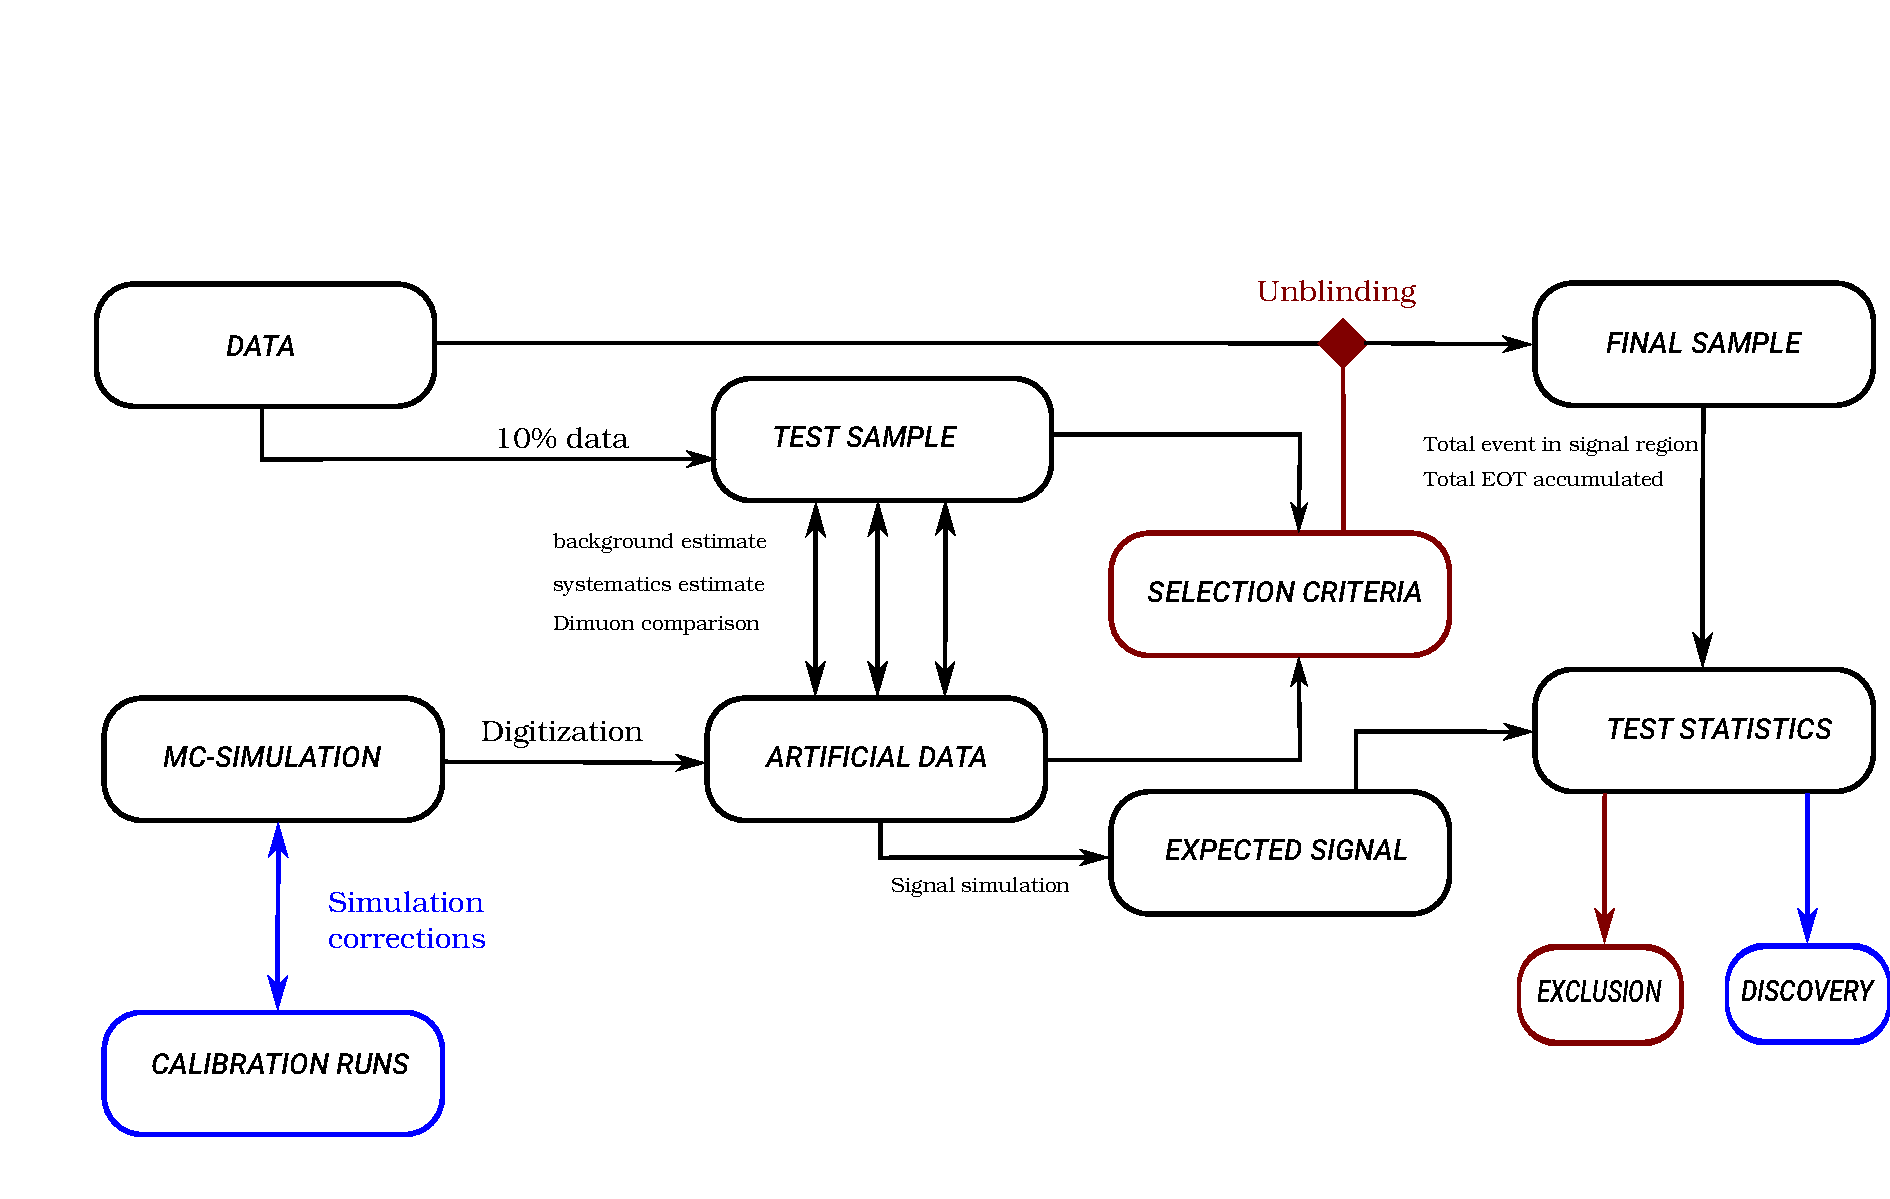
\includegraphics[scale=0.4]{\pdirthree/analysis-chart.pdf}
  \caption{Flowchart of the NA64 analysis.}
  \label{fig:analysis-chart}
\end{figure}

\section{Geant4 simulation of the experiment}
\label{ch3:sec:geant4}

The first ingredient for our analysis is Monte Carlo simulation used to reproduce the particle interactions in our setup. This can be divided into three subtasks:
\begin{enumerate}
\item Simulation of the particle interactions inside the NA64 setup.
\item Detailed description of the $A'$ physics.  
\item Detector response for each NA64 component.  
\end{enumerate}

The first task is handled by the Geant4 software\cite{AGOSTINELLI2003250} which includes geometry description, particle tracking, and run management. The end-user must provide an accurate description of the setup, a list of the interactions that need to be simulated, and the description of the primary particle type\footnote{For a list of available particles and the explanation of the numbering scheme, see \cite{geant4-pdg}}, initial momentum, and initial location.

The setup is described using different C++ classes to detail each detector geometry. A logical volume is assigned to each of them, which details the object properties. In most cases, this means the atomic number $Z$, the mass number $A$, and the density of the material. These properties were taken from the NIST database \cite{nist-database} unless more reliable information (coming from example from the manufacturer of the detector) was available. In some cases, for example to simulate the vacuum and the gas detectors, pressure and temperature are taken from in-situ measurements. Finally, detectors are placed in the simulation based on measurements I have done with a ruler (with a precision of $\sim$1 \si{\centi\meter}). For most detectors, this precision is sufficient to avoid any systematic error. For the trackers and the magnets, an additional measurement was performed by the H4 metrology team with a precision of 0.5 \mmi \cite{meterology-measurements}. This was later improved with an offline alignment procedure performed by the CORAL software \cite{ABBON2007455}. 

A physics list is then provided to describe the relevant set of interactions to simulate. The \textit{\textrm{FTFP\_BERT}} modular physics list was chosen, which is recommended for high-energy physics experiments \cite{ALLISON2016186}. This combines an excellent description of electromagnetic interactions and inelastic hadron-nucleus processes based on the Fritiof Parton model (FTF) \cite{Uzhinsky:2013hea}, Bertini intranuclear cascade \cite{Heikkinen:2003sc} and Precompound models \cite{Apostolakis:2009zz}. Because of the absence of a precise theory of QCD at low energy, the description of the inelastic scattering for hadrons can be a source of systematic errors in the experiment. This problem is addressed by correcting the model using data from the calibration runs, as detailed in Appendix.\ref{appC:sec:ftfp-modifications}.

Next, we add the $\DM$ physics description to Geant4. This is currently done by an additional C++ code that describes Dark Matter in a modular way. This allows for the description of many Dark Matter candidates inside the same framework. The code performs the following tasks:

\begin{enumerate}
\item Compute the total cross-section of $\DM$ emission as a function of the properties of the target nucleus (namely Z, A, and density $\rho$) and the primary energy.
\item Decide for each simulation step if $\DM$ is emitted.
\item Sample the energy and angle of the final state.
\item Compute the decay time in the laboratory system if the model predicts a visible decay and pass the information to Geant4.
\end{enumerate}

An instance of the Dark Matter class is called at the start of each run, initialized with specific parameters of $\epsilon$ and $m_{\DM}$. The method of the class is then called at each step involving\footnote{In some cases, this is called also for $\mu^-$/$\mu^+$ if the interaction is possible. In Sec.\ref{ch5:sec:muon-mode-setup} a setup to probe models with such interaction will be presented.} an $e^-$/$e^+$ to calculate the total cross-section and decide if emission is performed. After that, energy and angle are sampled using the calculated distribution $E_{\DM}(E_{e^-}, \theta_{\DM})$. In the case of the invisible mode, the energy of $\DM$ is subtracted from its parent particle and its momentum recalculated. No new particle is created inside the simulation, as the NA64 experiment assumes the decay product $\dmchi$ to punch-through the setup with no further interaction. In the case of the visible mode, the decay length of $\DM$ is computed as a function of its energy, mass $m_{\DM}$, and coupling $\epsilon$. An $\ee$ pair is created inside the decay volume by sampling the corresponding decay distribution in that region. A weight corresponding to the probability of $\DM$ to decay inside the fiducial volume is saved as meta-information of the event and later used to correct the signal yield.
The differential cross-section and energy spectrum of $\DM$ were initially calculated using the IWW-approximation described in Sec.\ref{ch1:sec:dm-u1model}. In our new analyses, this estimate was improved using a complete tree-level calculation of the cross-section, shown in Fig.\ref{fig:dm-iww-tl}. This correction decreased the expected signal yield for mass larger than 10 MeV but increased it for mass smaller than 5 MeV \cite{DMsimulation} (see Appendix.\ref{AppendixA}).

\begin{figure}[htb!]
  \centering
  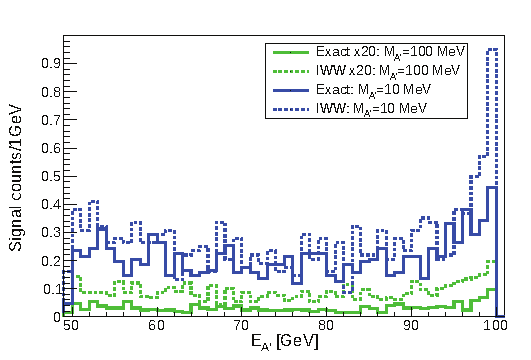
\includegraphics[width=\textwidth]{\pdirthree/DM-cs.pdf}
  \caption[IWW vs tree-level energy spectra]{Comparison of the energy spectrum of the emitted $\DM$ for a Dark Photon mass of 100 \mev and 10 \mev. The spectra are calculated using the IWW approximation (dotted line) and an exact tree-level calculation (continuous line) \cite{DMsimulation}.}
  \label{fig:dm-iww-tl}
\end{figure}


Finally, a biasing system was added to the code to increase the cross-section artificially. This is required to simulate efficiently the signal without the need of large statistics simulations. A correction factor $N_{norm}(\epsilon_{bias},m_{\DM})$ is calculated by the code and saved as metadata in the output. This factor is then used in the analysis of the simulations to correct for the artificial increase of the $e^- Z \to e^- Z \DM$ cross-section. To compute the signal rate $\dmpereot$ for a given MC-output, the following equation is used:

\begin{equation}
  \label{eq:1}
  \dmpereot = \frac{N_{norm}}{N} \times \sum^{n=N}_{i=0} \omega_i
\end{equation}

Where $N$ is the total number of events simulated, and $\omega_i$ is the weight associated with an event. For an event without $\DM$ production or that did not pass the selection criteria, this weight is zero. Else, the weight assumes a value between 0 and 1, which corresponds to the probability of $\DM$ to decay in the fiducial volume. For an invisible decay, the number is always 1, since no fiducial volume is present. For the case of the visible mode, the number is set to the probability of $\DM$ to decay within the acceptance of the setup. This corresponds to the integral of the decay spectrum between the last layer of the WCAL and the scintillator (S$_4$) placed at the end of the vacuum tube.

The final requirement to start the simulation is an input particle to start the whole machinery. 
To reproduce the beam reliably we use electron and hadron calibration runs to extract a profile. This is a work that was performed by me using the beam profile measured by the upstream Micromegas. Hadron and electron beams are quite different from each other\footnote{This feature can also be used to cross-check the beam contamination, see Sec.\ref{ch3:sec:dimuons}}. For the case of hadrons, the beam is parametrized as an ellipse, with total width in the X-direction of 14.5 $\mmi$ and 6 $\mmi$ in the Y-direction\footnote{X being the coordinate aligned with the direction of the bending inside the magnetic field}. In the case of electrons, the parameterization uses a 2D Gaussian distribution with $\sigma_x$=4.13 $\mmi$ and $\sigma_y$=1.4 $\mmi$. In both cases, the entrance angle of the particle is assumed to be uncorrelated with its initial position and is parameterized with a Gaussian of width $\sigma_r$=0.4 \mrad. These parameters were obtained by fitting the beam profile recorded by the two upstream Micromegas in the calibration runs in both projections. The two fits performed agreed within a 5\% error.
\clearpage
\subsection{Reconstruction and digitization}
\label{ch3:sec:geant4-digitization}

The output of Geant4 can be divided into three different categories:

\begin{itemize}
\item Energy deposited in the active area of a scintillator counter or a calorimeter.
\item Hit information of a particle passing through the active area of a tracking chamber.
\item MC truth information regarding the event, including all the kinematics of the $\DM$ if it was emitted.
\end{itemize}

Each time a step is computed inside a sensitive detector, the energy deposited in the volume is added to specific counters which are saved at the end of each event. At this point, some detector effects are already accounted for. Only the energy in the active part of each sampling calorimeter is recorded, and the total sum of the deposited energy is corrected using a calibration constant as it is done for the data. Additionally, Birks law \cite{NYIBULE2014141} is implemented in the HCAL to correct for the propagation of optical photons in the WLS, using an attenuation length of 30 \si{\centi\meter}. This accounts for the different light yields between $\pi^-$ and $\mu^-$, since in the case of $\mu^-$ the energy is deposited along the length of the detector evenly.

To collect the information for tracking detectors, every time a particle crosses the gas volume of a gas chamber, multiple pieces of information are saved:

\begin{itemize}
\item Particle x-y-z position at the beginning of the step.
\item The energy of the hit particle.  
\item The energy deposited in the gas during the step.
\item The PDG number of the particle \cite{particle-numbering-scheme}.
\end{itemize}

These data define a structure called \textit{MChit}, which is used by the reconstruction algorithm to reproduce both hits and tracks in the same format of the data. This algorithm was developed by me to improve the Digitization procedure. It works as follow:
\begin{enumerate}

\item Hits with energy deposited in the volume smaller than the minimum amount required to start the ionization are removed. Practically, this threshold was set to 2 keV based on previous studies performed for MM \cite{IGUAZ20121079}. A similar value is assumed for the GEM detector as well.
\item Multiple \textit{MChit} are merged if they are closer than a fixed distance. This is conservatively set to 2 $\mmi$  for MM and 1.75 $\mmi$  for GEM. The new x-y position of the hit is computed using the weighted average of the hits that are being merged, where the weight is defined by the energy deposited inside the gas.
\item The x-y coordinates are rotated to match the axes of the two detector planes using a simple matrix multiplication $u_{hit} = M_{uv}(\theta_{uv}) \cdot v_{hit}$ where $u_{hit}$ is the hit position in the detector coordinate system and $v_{hit}$ is the same vector expressed in the laboratory system. The Matrix $M_{uv}(\theta_{uv})$ is the rotation matrix of the $O(2)$ group where $\theta_{uv}$ is the angle between the axes of the detector and the ones of the laboratory system.
\item Each coordinate on the detector plane is treated separately. To reproduce the genetic multiplexing of the MM, each physical strip is mapped to its corresponding channels, and a 64-dimension vector is obtained as output. Noise is also added to each channel using the same pedestal measured in the sparse mode of the APV chips.
\item  The charge vector is used as input for the same clusterization procedure used for the data. In the MM detector, the clusterization is fully reproduced. The physical cluster is parametrized by a Gaussian, and the charge is distributed on the physical strips starting from the hit center. The total charge of the cluster is decided starting from the total energy deposited in the gas volume and converted into ADC counts. The conversion factor is computed using the data of the electron calibration runs. The procedure for the GEM is more direct and only involves the smearing of the initial true hit position using a Gaussian distribution with a width corresponding to the GEM hit resolution. This was estimated to be $\sigma_{GEM} \approx 80$ $\mum$ using the Three Layer Method \cite{Bortfeldt:2014vvt}.
\item After the clusterization is performed, two set $X_n$ and $Y_n$ of positions are extracted from the two planes and combined\footnote{In the most common case of just a single primary present upstream the ECAL, this association is trivial since only one hit per plane is present.} in the set of hit candidates $(X;Y)_n$. A hit number per plane larger than five, other than being rare ($\lesssim$0.1\%), is not relevant for $\DM$ searches and hence rejected in the reconstruction. The hits are then used as input of the tracking or vertexing procedure, which is the same for both simulation and data. The total momentum of a track is calculated from the displacement after passing through the magnetic field of the MBPL (see Appendix.\ref{AppendixD}). The vertex reconstruction procedure is described in more detail in Sec.\ref{ch3:sec:vis-mode-tracking}.
\end{enumerate}

Completed the procedure, these quantities are saved in a tree structure implemented in ROOT \cite{root} that is equivalent to the one used for the data. A shower profile analysis is also performed at this step (see Sec.\ref{ch3:sec:bkg-ecal-profile}) and added to the tree. This design allows using the same analysis to study both MC and data using the same tool.

\section{Monte Carlo validation using $\gamma + Z \rightarrow \mu^+ \mu^-$ events}
\label{ch3:sec:dimuons}

The $\emu$ interaction consists of the rare production of a $\mu^+\mu^-$ inside an em-shower after a photon interacts with a nucleus inside the target. The process of pair production is equivalent for all charged leptons (e,$\mu$,$\tau$) and has a cross-section in the order of $\sigma_{pair} \sim 4Z^2\alpha r^2_c$. Compared to the more frequent $\ee$ production, this interaction is suppressed by a factor ($m_e$/$m_{\mu}$)$^2$ = 2.34 $\times 10^{-5}$ because of the larger muon mass. This process is used both to validate the MC simulation and to correct the expected signal yield, as it shares many similarities with events involving a Dark Photon emission:

\begin{enumerate}
\item Rare process produced inside an em-shower.
\item In first approximation, it can be computed inside the QED framework\footnote{This is not technically the case for $\DM$, but given that it is generated by an equivalent U'(1) symmetry, the precision will be the same.}, hence with high precision.
\item The process penetrates very efficiently both the target and the HCAL modules. Each $\mu^{\pm}$ loses an energy $<$\SI{250}{\mega\electronvolt} after its passage through the target, and $\sim$1.3 $\gev$ for each HCAL module encountered. 
\item The energy spectrum of the emitted $\mu^+\mu^-$ left in the target covers the same region of the signal ($0 < E_{ECAL}^{\gamma \to \mu^+ \mu^-} < \SI{90}{\giga\electronvolt}$) \cite{dimuon-mc}.
\end{enumerate}

Additionally, because of the double MIP signature that the $\emu$ interaction leaves inside the VETO and the HCALs, this interaction can be easily distinguished from a signal event.

In Geant4, the process is described starting from the formula \cite{dimuon-mc}:

\begin{equation}
  \label{eq:sigma-dimuon}
  \sigma_{tot}^{\gamma \to \mu^+ \mu^-}(E_{\gamma}) = 4\alpha Z^2 r^2_c\int^{x_{max}}_{x_{min}} \left(1 - \frac{4}{3}x_+x_- \right) \log{W}dx_+
\end{equation}

Where $x_+$ the fraction of energy of the original $\gamma$ being transferred to the $\mu^+$ and $W$ is a function of $x_+$,$E_{\gamma}$, and the Z, A of the element, which also takes into account both the atomic-screening using the Thomas-Fermi model and the finite size of the nucleus. Numerical values for this are provided in \cite{dimuon-mc}. To increase computation speed, a parameterization of Eq.$\ref{eq:sigma-dimuon}$ is used instead, with a precision greater than 2\%. After the dimuon pair is generated, the amount of energy transferred to the $\mu^+$ is decided by sampling the differential cross section\footnote{In this case, just the argument of the integral in Eq.\ref{eq:sigma-dimuon}} and the new particles are produced in Geant4. Since the interaction is approximately elastic, the relation $E_{\gamma} = E_{\mu^+} + E_{\mu^-}$ is used for the computation.

For a comparison between data and MC, $\emu$ interaction are collected from the complete sample collected for both visible and invisible mode using the criteria $\SI{1.2}{\giga\electronvolt} < E_{HCAL}^{1,2,3} < \SI{6.35}{\giga\electronvolt}$ (passage of two MIPs in all HCAL modules). All selection criteria, excluding the cuts on VETO or W2 (for the visible mode), are then applied to the data sample. The obtained energy spectrum in the target for MC and data are normalized to the same value to compare them. After that, the two distributions are normalized to the number of EOT collected.
Each bin is compared between data and MC and their ratio is computed:

\begin{equation}  
  \label{eq:RR-factor}
  \begin{aligned}
  &R_{data/MC}^i = \frac{n_i^{ECAL}}{n_{tot}^{ECAL}} \\
  &RR_i = R_{data}^i/R_{MC}^i
  \end{aligned}
\end{equation}

Inside the MC, the signal yield is corrected using $RR_i$ in each bin of the $E_{ECAL}$ spectrum. Such corrections are different between runs and are mostly affected by the intensity of the beam and the variation of the trigger-threshold in the Pre-Shower detector during data taking. The signal yield is reduced by 5\%-10\% after these corrections are applied. Differences in re-weighting between runs collected at the same intensity are taken as systematic errors, which amount to a maximum of 7\%\footnote{The error has a small dependence from the $\DM$ mass. For example for masses of $\simeq$10 MeV this error amount to 5\% \cite{na64-prd}.}. An example of such comparison is shown in Fig.\ref{fig:dimuon-comp-invis}.

\begin{figure}[tbh!]
  \centering
  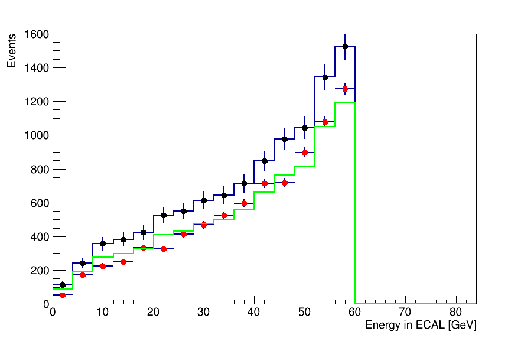
\includegraphics[width=0.45\textwidth,height=0.43\textwidth]{\pdirthree/dimuon-ecal-comp.pdf}
  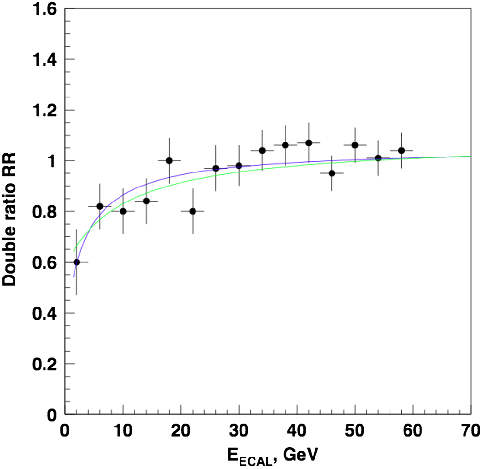
\includegraphics[width=0.45\textwidth,height=0.4\textwidth]{\pdirthree/dimuon-RR-comp.pdf}
  \caption[Dimuon spectra in ECAL for data and MC.]{Left: Distribution of energy deposited in the ECAL target by the scattered electron from the reaction $\emu$ selected from data (red dot) and MC generated event (green line). Data and MC are normalized to the same number of events. The un-normalized MC distribution is also shown with the corresponding error on the top histogram (blue line). Right: Ratio $RR$ between MC and data efficiency of dimuon production as function of the ECAL energy deposited. The two color curves shows examples of empirical distribution of the values \cite{na64-prd}.}
  \label{fig:dimuon-comp-invis}
\end{figure}

\section{Background rejection methods}

Part of my thesis work was aimed to study and improve the background rejection. In this section, I will describe two methods I developed for this purpose.

The first one exploits the emission of electron synchrotron radiation(SR) during their passage through a magnetic field. The detection of the SR allows for the electron identification (ID). The nature of this radiation is described in more detail in Appendix.\ref{appB:sec:sr}, together with the most relevant equations to describe its phenomenology. The method was tested using BGO crystals during the test beam in 2015 and in the run performed in 2016. This method resulted in a total hadron suppression of $\simeq 10^{-5}$ published in \cite{Depero:2017mrr}. In order to cope with higher fluxes, the SRD based on BGO was replaced by a shashlik type calorimeter.

The second method consists of a shower profile analysis to check the compatibility of the energy deposited in each ECAL cell with the one predicted for an em-shower. A set of measurements performed using calibration runs were used to build a model to predict the energy deposit as a function of the impact point of the incoming particle extrapolated from the Micromegas.  This method was documented in an official NA64 note \cite{na64-shower-profile}, and achieved a background suppression of $\simeq 10^{-3}$.

\subsection{Heavy charged particle rejection using synchrotron radiation}
\label{ch3:sec:bkg-srd}

The identification of heavy charged particles is one of the main tools to suppress the contamination of $\pi^-$,$K^-$, and $\mu^-$ present in the beam. The working principle of this method is based on the fact that a particle traveling through a magnetic field will emit synchrotron radiation. The total power after a full cycle can be calculated with the formula:

\begin{equation}
  \label{eq:srd-power}
  P = \frac{q^2 c}{6 \pi R^2}\frac{E^4}{m^4}
\end{equation}

Here $R$ is the bending radius experienced by the particle inside a magnetic field $B$ perpendicular to its velocity. From this equation, we see that the total power scales to $P\sim E^4/m^4$. Therefore, the technique is suitable for high-energy particle, as the signal will be boosted, and can be used to separate particles with large differences in the mass spectrum. The mass of all charged particles excluding the electron is so large that no detectable radiation is emitted at the primary energy used in NA64. 

Simulation of the expected SR signal was performed with the Geant4 package \cite{ALLISON2016186,1610988,AGOSTINELLI2003250}. The BGO saturation was included using Birks' law with the constants taken from \cite{AVDEICHIKOV2002251}.

The expected SRD spectra for pions and electrons with energies of 50 GeV and 100 GeV is shown in Fig. \ref{fig:SRspectrum}. From this plot, one can see the dependence of the emission spectra on the incoming electron energy for the realistic experimental conditions. Moreover, the comparison between the spectra of pions and electrons illustrates clearly the principle of this technique. For pions, one can see that the probability of detecting an event with energy above 1 MeV is about $\lesssim 10^{-3}$.
These SR-like signals originate from the interactions of the incoming pions with materials placed along the beamline. Although in first approximation the energy transfer due to ionization is in the order of few \si{\kilo\electronvolt}, rare high-energy transfer is also possible. The distribution of such secondary electrons (also called $\delta$- or knock-off-electrons) with
kinetic energy $T\gg I$, where $I$ is the mean excitation energy of the
atom/molecule, for a particle with velocity $\beta=v/c$ and charge $z$
passing through a material with atomic number $Z$, mass number $A$ and
thickness $dx$ is described by \cite{review-particle-physics}:
\begin{equation}
\frac{d^2N}{dTdx} = \frac{1}{2}K z^2 \frac{Z}{A}
\frac{1}{\beta^2}\frac{F(T)}{T^2}
\label{eqn:knock-on}
\end{equation}
The constant $K$ is defined as $K=4\pi N_A r_e^2 m_e c^2$ where N$_A$ is
the Avogadro's number, $r_e$ is the classical electron radius and $m_e$
the electron mass.
$F(T)$ is a spin-dependent factor, which in our case for $T \ll W_{max}$
is very close to unity. W$_{max}$ is the maximal energy transfer in a single collision to the
electron:
\begin{equation}
W_{max} = \frac{2m_e c^2 \beta^2 \gamma^2}{1+ 2\gamma m_e/M+(m_e/M)^2}
\end{equation}
For a $\pi^-$ at 100 GeV, $W_{max}$ is roughly 1 GeV which
covers completely the energy range where synchrotron radiation is
emitted. Eq.\ref{eqn:knock-on} is valid in the range $I\ll T \leq W_{max}$.
 \par 
Furthermore, Geant 4 reproduces the critical energy $E_c$ which divides the spectrum into two parts of equal power is:
\begin{equation}
E_c = \frac{3 \hbar c \gamma^3}{2R}
\end{equation}
with the reduced Plank constant $\hbar$ and the bending radius $R$. 
 For 100 GeV electrons in the  $B=1.7$ T bending field this corresponds to $E_c\sim$11.35 $\mev$. The expected mean energy of a synchrotron photon $E_m=E_c/\pi\simeq 3.6$ $\mev$ is in very good agreement with simulation. The number of photons emitted per revolution in this energy range in the field of \SI{7}{\tesla\meter} is defined as:
\begin{equation}
N_\gamma = \frac{5 \pi \alpha}{\sqrt{3}}\gamma
\end{equation}
where $\alpha$ is the fine structure constant. 
By scaling this equation for the fraction of the circle where the particles are inside the magnetic field, one obtains a mean number of emitted photons of about 24.
The SRD geometrical acceptance is about one third,  thus one can estimate that the sum of deposited energy is approximately 29.35 $\mev$ in good agreement with the results of the simulation as shown in Fig.\ref{fig:SRspectrum}. 
 
\begin{figure}[htb!]
\centering
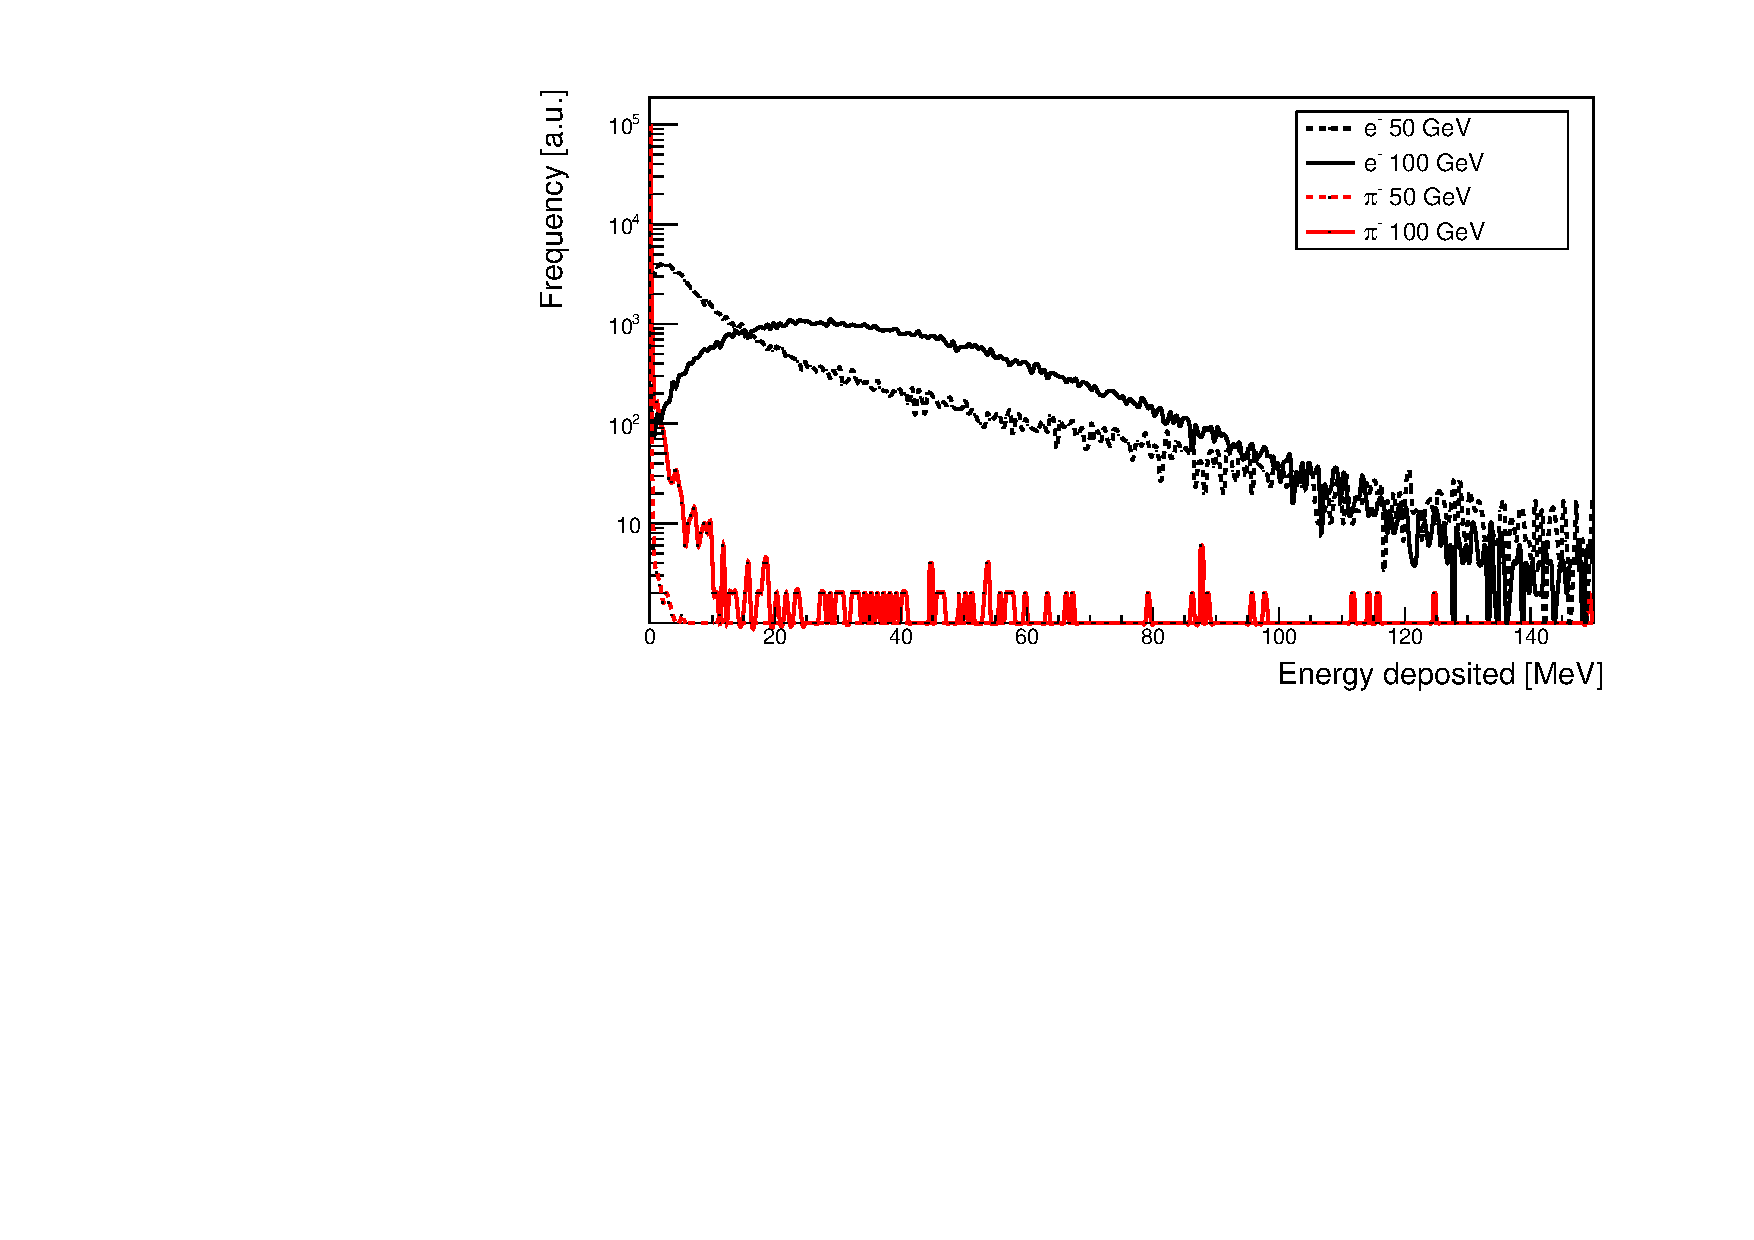
\includegraphics[width=1.\textwidth]{\pdirthree/comp_spectra.pdf}
\caption[SR spectrum for different energy detected in the SRD]{Result of the Geant 4 simulation for the energy detected by the SR detector for 50/100 GeV e$^-$(black dashed/solid line) and 50/100 GeV $\pi^-$ (red dashed/solid line).}
\label{fig:SRspectrum}
\end{figure}

The SRD detector was tested during the physic run in July 2016. The two BGO rows are parallel to the primary beam direction as shown in Fig.\ref{fig:newgeo}. The dipole magnets installed in series produce a total integrated magnetic field of 7 \si{\tesla\meter} \cite{Banerjee:2016tad} resulting in a nominal displacement for the incoming electrons at the SRD/ECAL positions of 31/34 cm from the undeflected beam axis. The SRD was placed between the undeflected and the deflected beam axis at a distance of approximately 9 cm from both (Fig.\ref{fig:newgeo}). This separation minimizes the possibility for Bremsstrahlung photons and neutral particles produced by interactions of the beam particle with materials upstream and for particles in the beam halo to hit the SRD. In fact, such interactions result in the saturation of the SRD with a significant loss of efficiency due to the long decay time of the BGOs.

The two crystals facing the beam (labeled 3 and 7 in Fig. \ref{fig:newgeo}) detect most of the energy emitted by synchrotron radiation. We will refer to those as SRD BGO. The remaining six crystals are used to detect events with high-energy deposition in the SRD. In particular, the last two crystals of each row (labeled 0 and 4 in Fig. \ref{fig:newgeo}) detect some energy only in the case of very energetic Bremsstrahlung events and thus can be used as a veto (see Fig.\ref{fig:newgeo}). The six crystals after the SRD BGOs act also as a shield from backscattering particles coming from the ECAL suppressing pions by an additional order of magnitude. Finally, in this geometry it is possible to use the coincidence of the two SRD BGO crystals to improve the tagging of synchrotron photons by rejecting knock-on electrons produced by incoming pions. In fact, synchrotron radiation has a homogeneous spectrum in the whole arc described by the primary and deflected beam, and thus a signal is detected in both SRD BGOs. On the contrary, electrons generated by a $\pi^-$ undergoing ionization will mostly leave energy only in a single crystal as illustrated in Fig. \ref{fig:newgeo}. 
With the requirement of detecting in both SRD BGOs an energy deposition above a 1 MeV the suppression factor is improved up to a level of $10^{-5}$.



\begin{figure}[htb!]
  \centering
  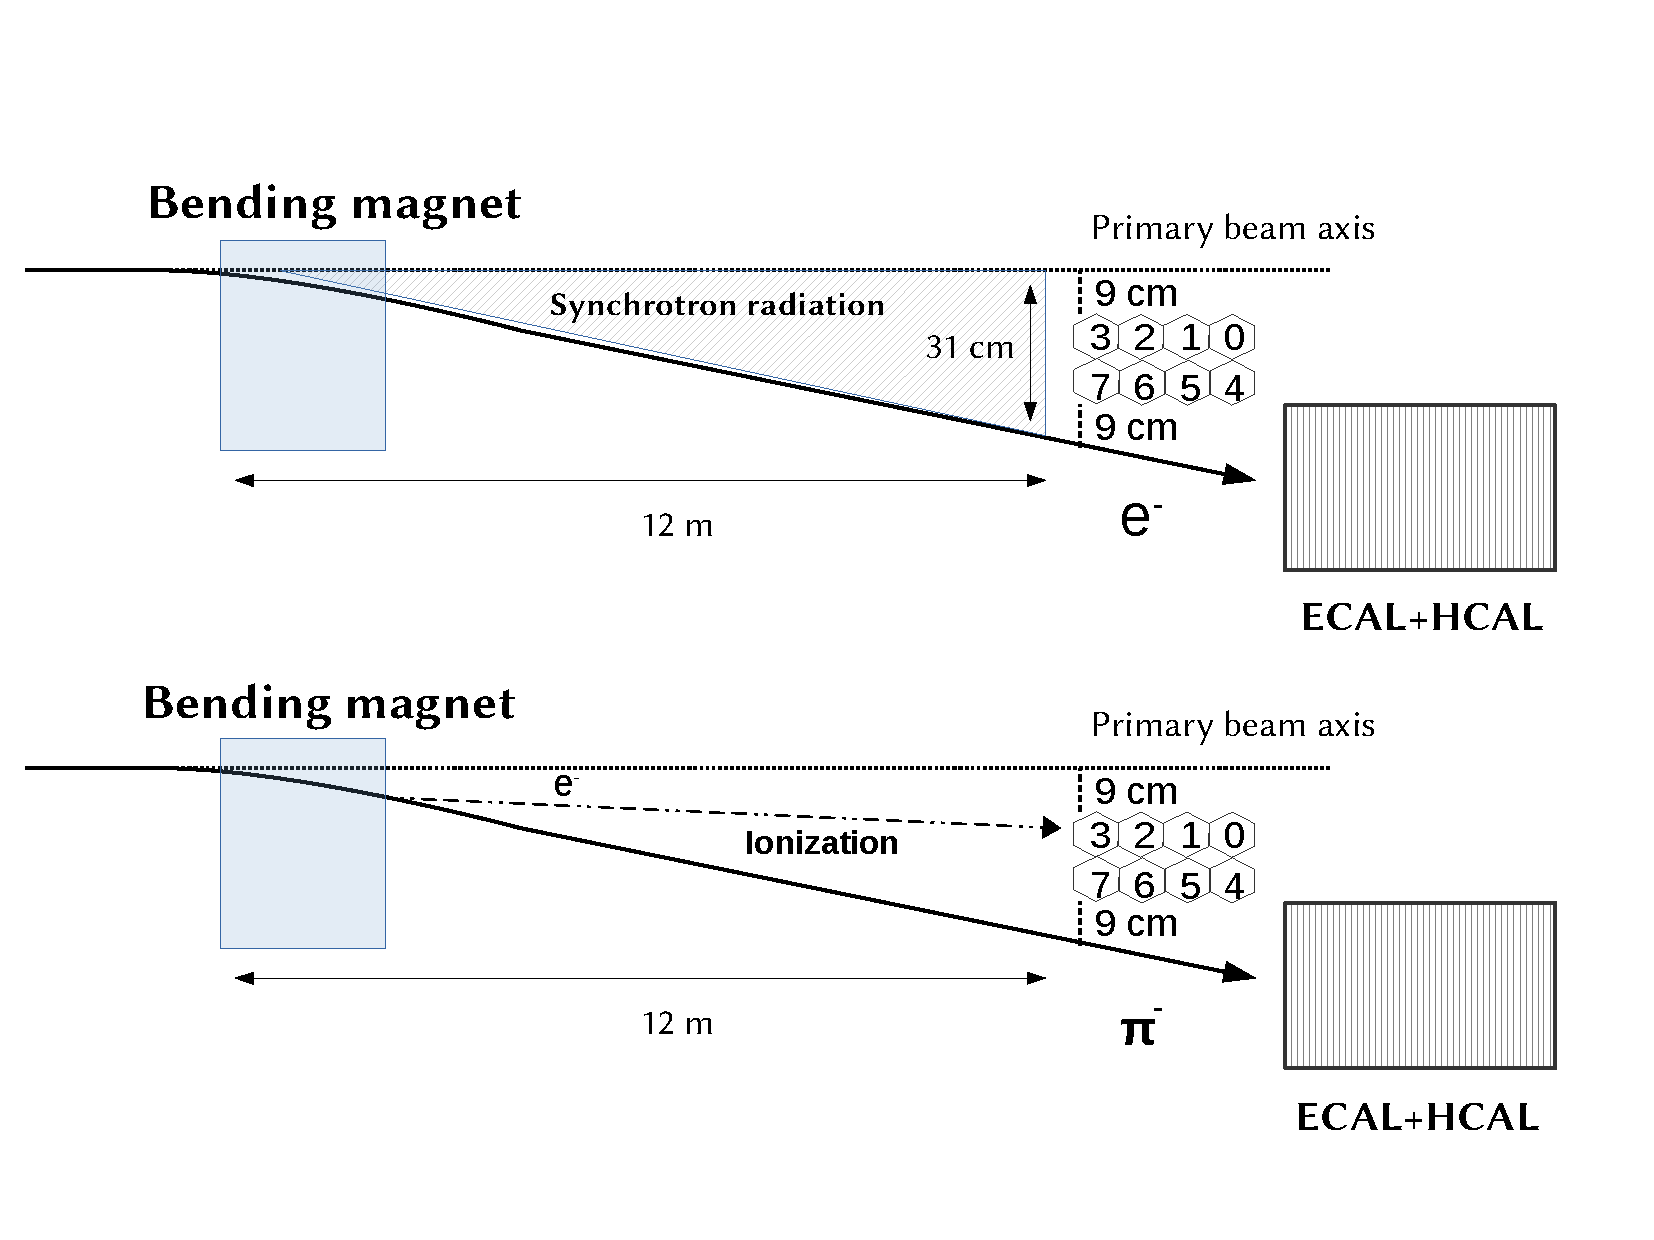
\includegraphics[width=.9\textwidth]{\pdirthree/sketch.pdf}
  \caption[Geometry of the BGO crystals]{Geometry of the BGO crystals. Crystals 7,3 (SRD BGO) collect most of the synchrotron radiation spectrum. Crystals 4,0 (VETO BGO) on the other hand are effected only in case of a high-energy event and are thus used as a veto. The remaining crystals serve as a shield for the SRD from backscattering particles coming from the ECAL. Top: illustration of an event leaving a SR signal in the SRD. Bottom: illustration of a SR- like signal in the SRD for a knock-on electron produced by pions.}
\label{fig:newgeo}
\end{figure}

Data with a 100 GeV $\pi^-$ beam were taken to have a direct measurement of the suppression factor achievable through synchrotron radiation measurements. The beam intensity was 5.3$\times 10^4$ particles per spill. The additional requirement of an energy deposition below 60 GeV in the ECAL was applied in order to completely reject electrons from the $\pi^-$ sample of $\sim 10^5$ collected events.

For the 100 GeV electron beam run, a total of 220 spills were recorded with an intensity of 3.4$\times 10^5$ EOT/spill. 
The same trigger used in the pion run was used for the electron data.
In this case, however, in order to reduce the pion contamination events with total energy deposition in ECAL + HCAL above 90 GeV but with less than 20 GeV energy in the HCAL were used.  

The energy spectra recorded by the SRD BGO with electrons and pions are shown in Fig.\ref{fig:comp_spectra}. The SR spectra obtained with the electron beam are used to perform the BGO calibration by comparison with the simulation. With this method, a very good agreement of data and MC is achieved (see plot on the left of Fig.\ref{fig:comp_spectra}). As a cross-check, using the obtained calibration constants, the data from the pion beam impinging directly on the SRD are fitted with a Landau distribution. The obtained peak position of 60 MeV is in good agreement with the prediction of the MC. 

Time coincidence of signals above the energy threshold of 1 MeV from both SRD counters is required and high-energy Bremsstrahlung events are removed using the veto BGO.
The suppression of synchrotron radiation emission detected for pions compared to electrons is clearly visible by comparing the two plots. For the electron spectrum, a 1\% pileup beam events have been added to the simulation as predicted for the given spill intensity and with the known decay time of BGOs.  Both spectra are in very good agreement with the simulation.

\begin{figure}[htb!]
  \centering
  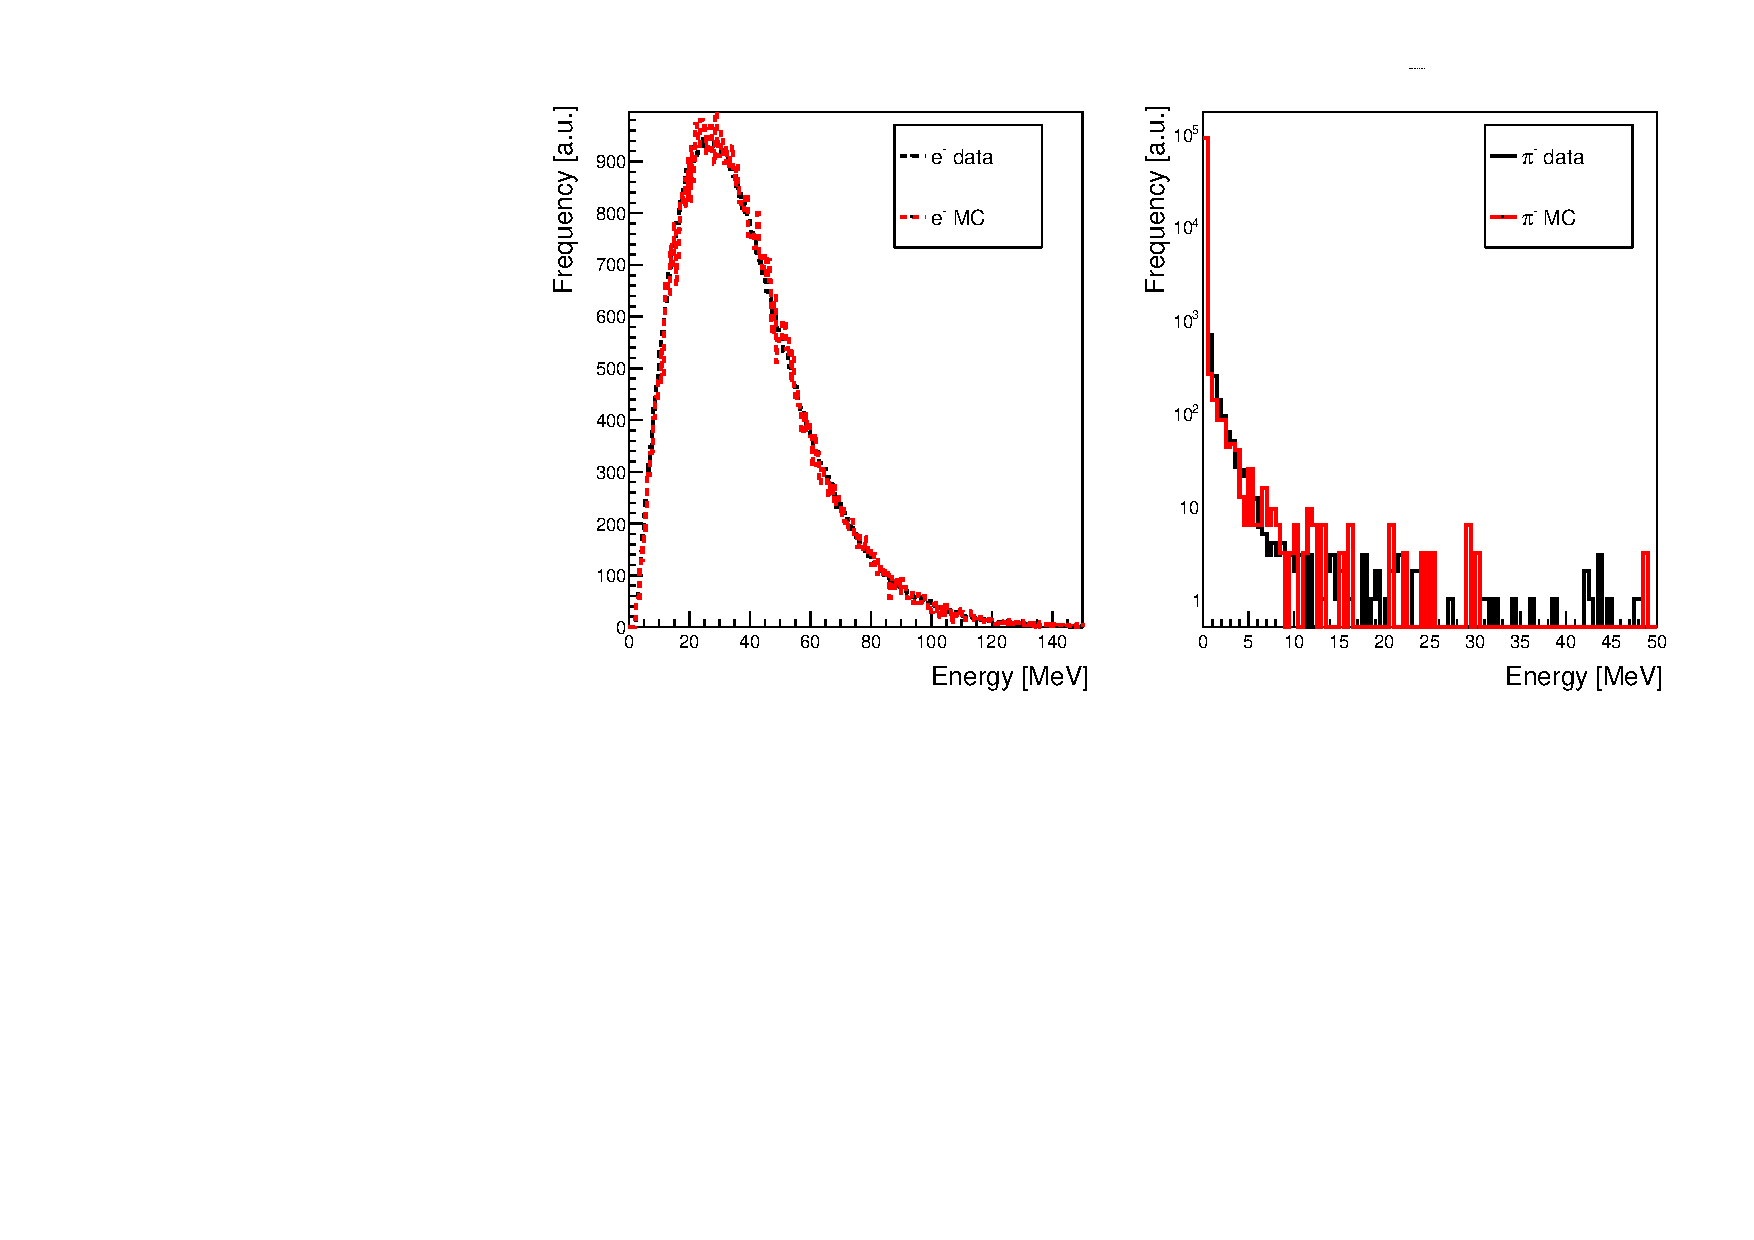
\includegraphics[width=1.\textwidth]{\pdirthree/spectra_tot.pdf}
  \caption[SRD comparison between data and MC]{Comparison between data and simulation (MC) of the synchrotron radiation spectrum detected for 100 GeV electrons (left) and pions (right). }
  \label{fig:comp_spectra}
\end{figure} 

\begin{figure}[htb!]
  \centering
  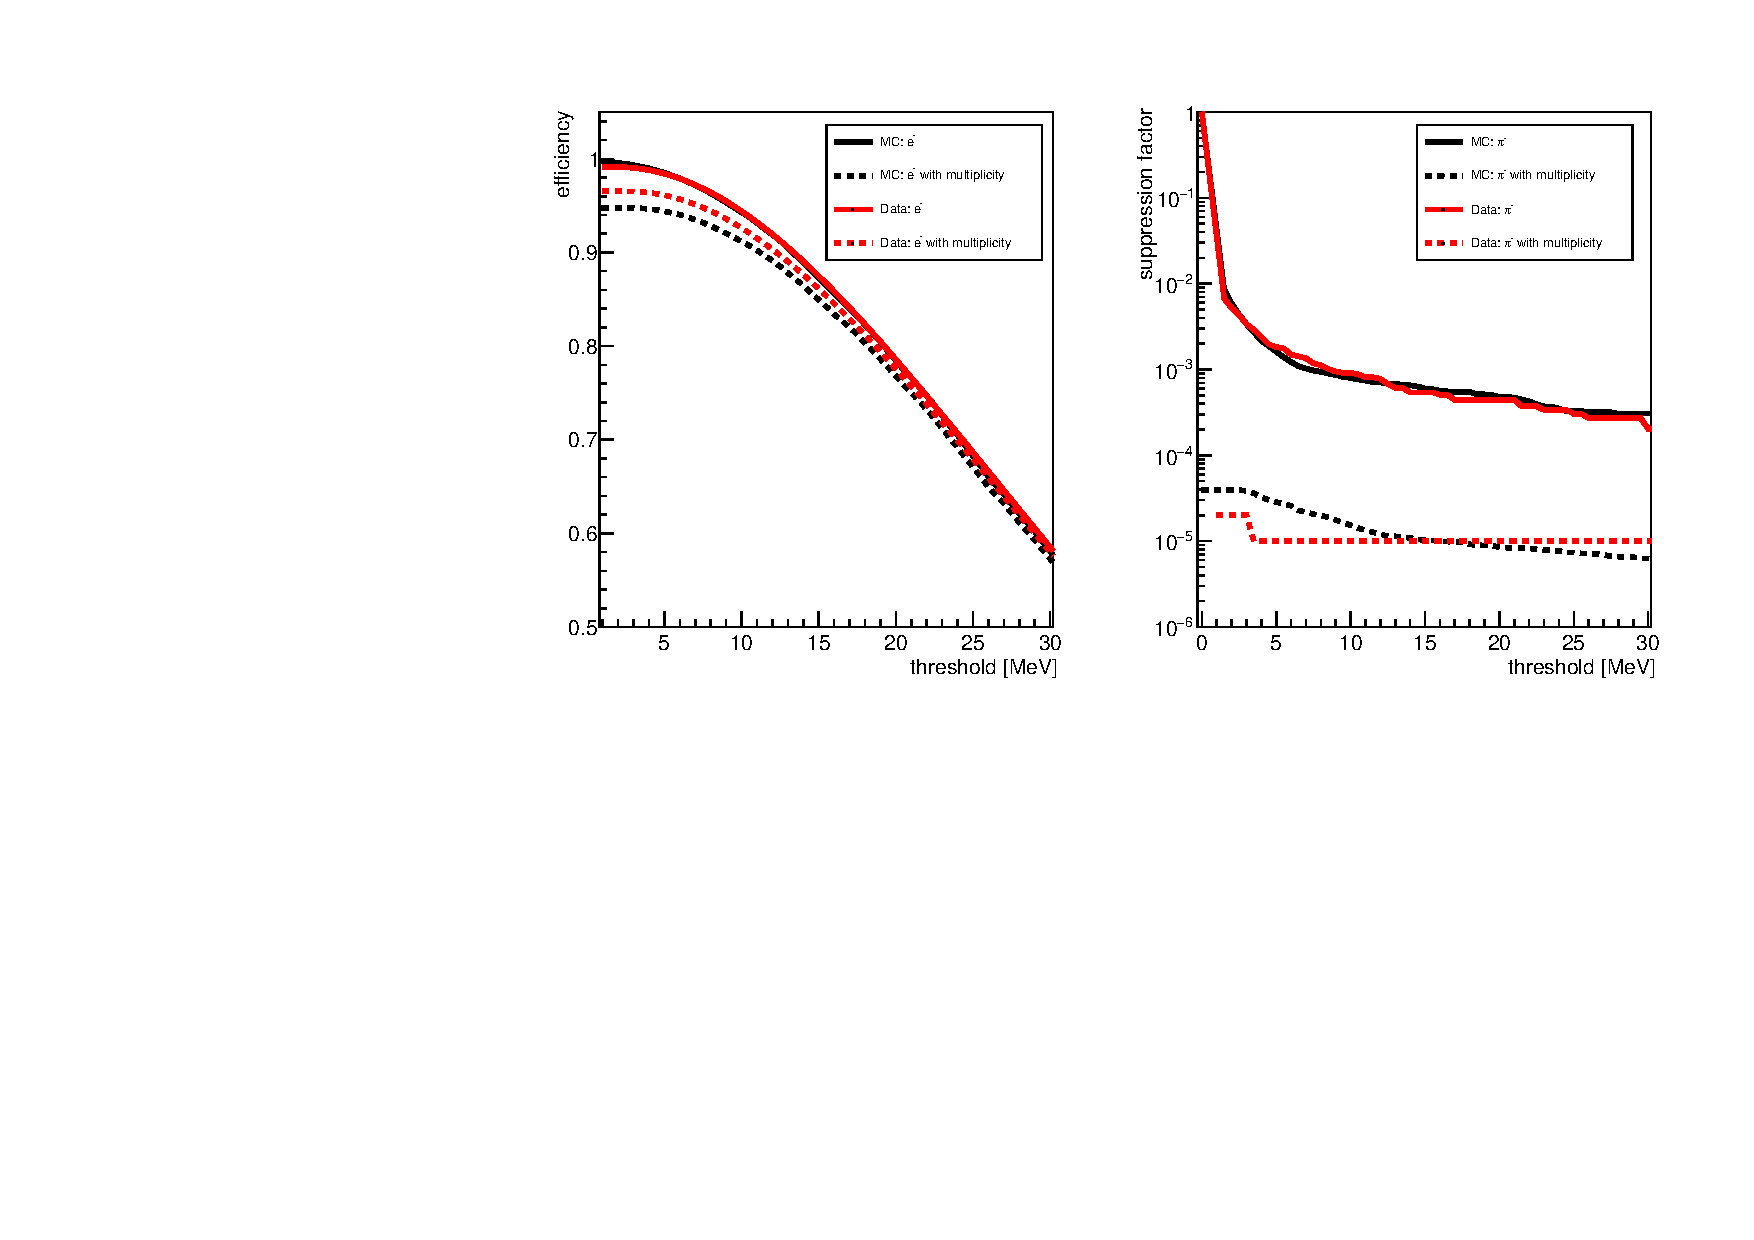
\includegraphics[width=1.\textwidth]{\pdirthree/sup_mult.pdf}
  \caption[efficiency and rejection power of the SRD cut]{Left: Comparison between data and simulation (MC) for electrons of the efficiency as a function of the threshold set on the total energy deposited in the SRD BGO and for the requirement that this is deposited in each single crystal (multiplicity). Right: Comparison between data and simulation for pions and electrons of the suppression factor as a function of the threshold set on the total energy deposited in the SRD BGO and for the multiplicity requirement.}
  \label{fig:sup_mult}
\end{figure}

The efficiency for the electrons and the suppression factor for the pions are plotted in Fig. \ref{fig:sup_mult} as a function of the threshold on the energy deposited in the SRD. We distinguish between two cases:
\begin{enumerate}
\item The threshold is set on the total energy deposited in the SRD.
\item Both SRD signals have to be in-time and above the threshold of 1 MeV (multiplicity requirement).
\end{enumerate}
One can see that applying the criterion 2) the efficiency only decreases slightly compared to 1), while the suppression factor for pions is dramatically increased (by two orders of magnitude).
This is also underlined by Table  \ref{tab:hits} where the fraction of events with different hit multiplicity in the SRD BGO for both pion and electron runs are reported.

\begin{table}[hbt!]
\begin{center}
\begin{tabular}{cccc}
Events hit multiplicity  (\%) & 0 BGO  & 1 BGO & 2 BGOs\\
\hline
Pions & $98.77$ & $1.21$ & $1.4\times10^{-3}$  \\
Electrons & $2.4\times10^{-1}$  & $2.60$ & $97.37$ \\
\end{tabular}
\end{center}
\caption[Fraction of pion and electron events for different hit multiplicity in the SRD from the data]{Fraction of pion and electron events for different hit multiplicity in the SRD from the data.}
\label{tab:hits}

\end{table}

\FloatBarrier\noindent
\subsection{Hadron rejection using electromagnetic shower profile}
\label{ch3:sec:bkg-ecal-profile}

The transversal segmentation of the ECAL offers another tool for hadron rejection. The idea is to discriminate between an em-shower profile and an hadronic one using a $\chi^2$-test. A shower profile database can be built by correlating the hit position (x,y) on the ECAL with the fraction of energy deposited in each ECAL cell. The method used to build this database is detailed in Appendix.\ref{Appb:sec:make_profile}. A predicted value of energy deposited in each ECAL cell is extracted and compared to the one measured in the event. The compatibility between the predicted profile and the measured one can be tested using the $\chi^2$-distribution:

\begin{equation}
  \chi^2 = \sum^{9,36}_i \left(\frac{E_{pred}^i(x_{hit},y_{hit})-E_{mes}^i}{\sigma^{i}_{pred}(x_{hit},y_{hit})}\right)^2
  \label{eqn:chi}
\end{equation}


\begin{description}
\item[$E_{pred}^i$]: is the energy predicted by the profile of cell
  $i$
\item[$E_{mes}^i$]: is the energy measured in the cell $i$
\item[$x_{hit},y_{hit}$]: coordinates of the hit position of the
  particle in the ECAL plane
\item [$\sigma^{i}_{pred}$]: error estimated for the predicted energy
  in cell $i$
\end{description}


Two different summation indexes are used for the two different cases
where only the cells surrounding the central one hit by the beam are
used for the test (total of 9 cells) and the case where all the cells
are used (total of 36, see Fig.\ref{fig:ecal_example}).

\begin{figure}[h!]
  \begin{center}
    \includegraphics[scale=0.47,page=4]{\pdirthree/ecal_example.pdf}
  \end{center}
  \caption[ECAL sketch]{sketch of the 36 cells of the ECAL. The central cell 3X3
    were the beam is directed is plotted in red, while the cells
    surrounding it are plotted in green. On the bottom-right an
    example of how a profile for a cell looks like in the MC.}
  \label{fig:ecal_example}
\end{figure}

To test the rejection power and the efficiency of the
method the algorithm described above was used for 3 type of samples\footnote{The database was generated using the electron  calibration runs 2363, 2182, 2410, 2406, 2438. A complete description of such runs can be found in \cite{na64-runs}. }:
\begin{itemize}
\item $\simeq$1.2$\times 10^{6}$ events acquired with an electron calibration run\footnote{run 2363}.
\item $\simeq$5$\times 10^{5}$ events acquired with an hadron calibration run\footnote{run 2204}.
\item $\simeq$8$\times 10^{5}$ events acquired using physical trigger at maximum H4 beam intensity.\footnote{run 2241, corresponding EOT before trigger suppression $\simeq 4 \times 10^{8}$}
\end{itemize}

The comparison of the normalized $\chi^2$-distribution between
electron and hadrons calibration runs using information from all 36
cells is shown in Fig.\ref{fig:chi2}. Note that electrons reproduce
the expected shape of a $\chi^2$-distribution while for hadrons we
observe a displaced one incompatible with the one produced by
electrons.  The rejection and efficiency of a cut
$\chi^2 < \chi^2_{cut}$ are shown in Fig.\ref{fig:eff}. For
a benchmark cut $\chi^2_{cut} = 2$ the efficiency calculated in run 2363
was $\sim 0.94$ with a rejection factor of $1.2\times 10^{-3}$
extracted from the hadron run 2204.

Using the 9 central cells (Fig.\ref{fig:ecal_example}) shifts the distribution
to the left and reduces its spread ( Fig.\ref{fig:chi}) due to the
smaller number of degrees of freedom. The two methods have an overall
comparable efficiency as can be seen in Fig.\ref{fig:eff} but smaller
rejection power when the benchmark cut is applied.  For $\chi^2_{cut}=$2, the efficiency measured using only
central cells was of $\sim 0.93$\ and a rejection factor of $3.1\times 10^{-3}$.


\begin{figure}[h!]
  \begin{center}
    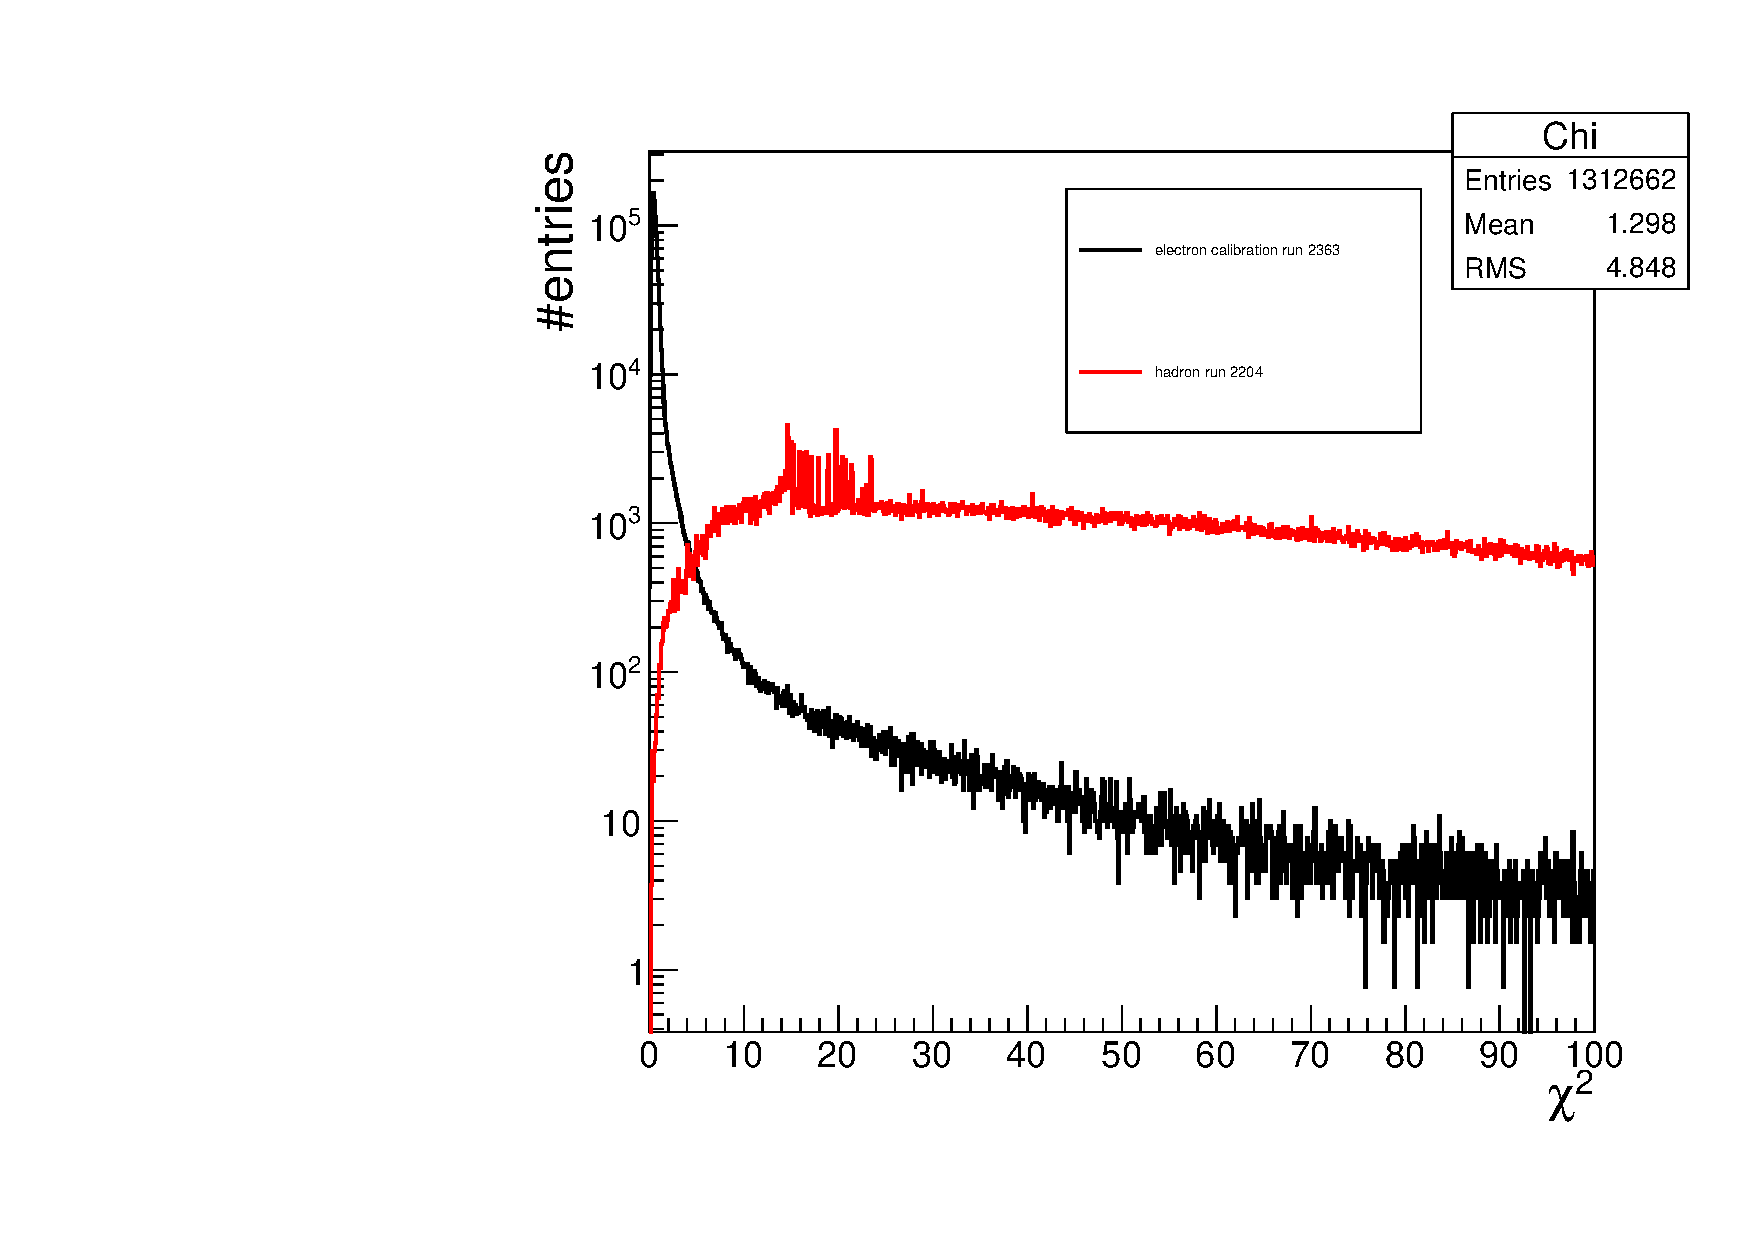
\includegraphics[width=0.95\textwidth,height=0.8\textwidth]{\pdirthree/chi_comp.pdf}
  \end{center}
  \caption[Comparison between $\chi^2$ distribution, electron and hadron calibration run]{Comparison between $\chi^2$ distribution generated from an electron calibration run (black) and hadron calibration run (red).}
  \label{fig:chi2}
\end{figure}

\begin{figure}[h!]
  \begin{center}
    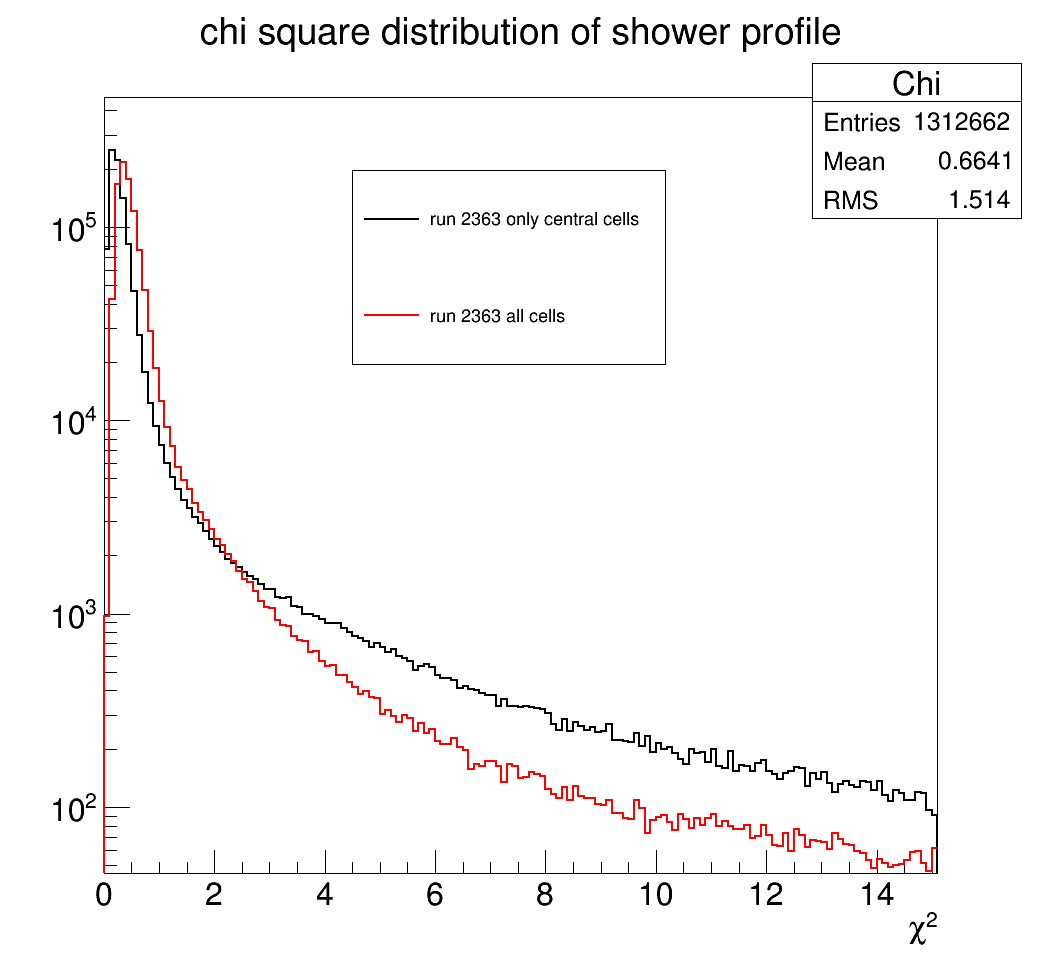
\includegraphics[width=0.95\textwidth,height=0.8\textwidth]{\pdirthree/plot_comp_cells.png}
  \end{center}
  \caption[Comparison between $\chi^2$ distribution for different ECAL configurations]{Comparison between $\chi^2$ distribution generated from an electron calibration run considering only central cells (black) and considering all 36 cells (red).}
  \label{fig:chi}
\end{figure}

\begin{figure}[h!]
  \begin{center}
    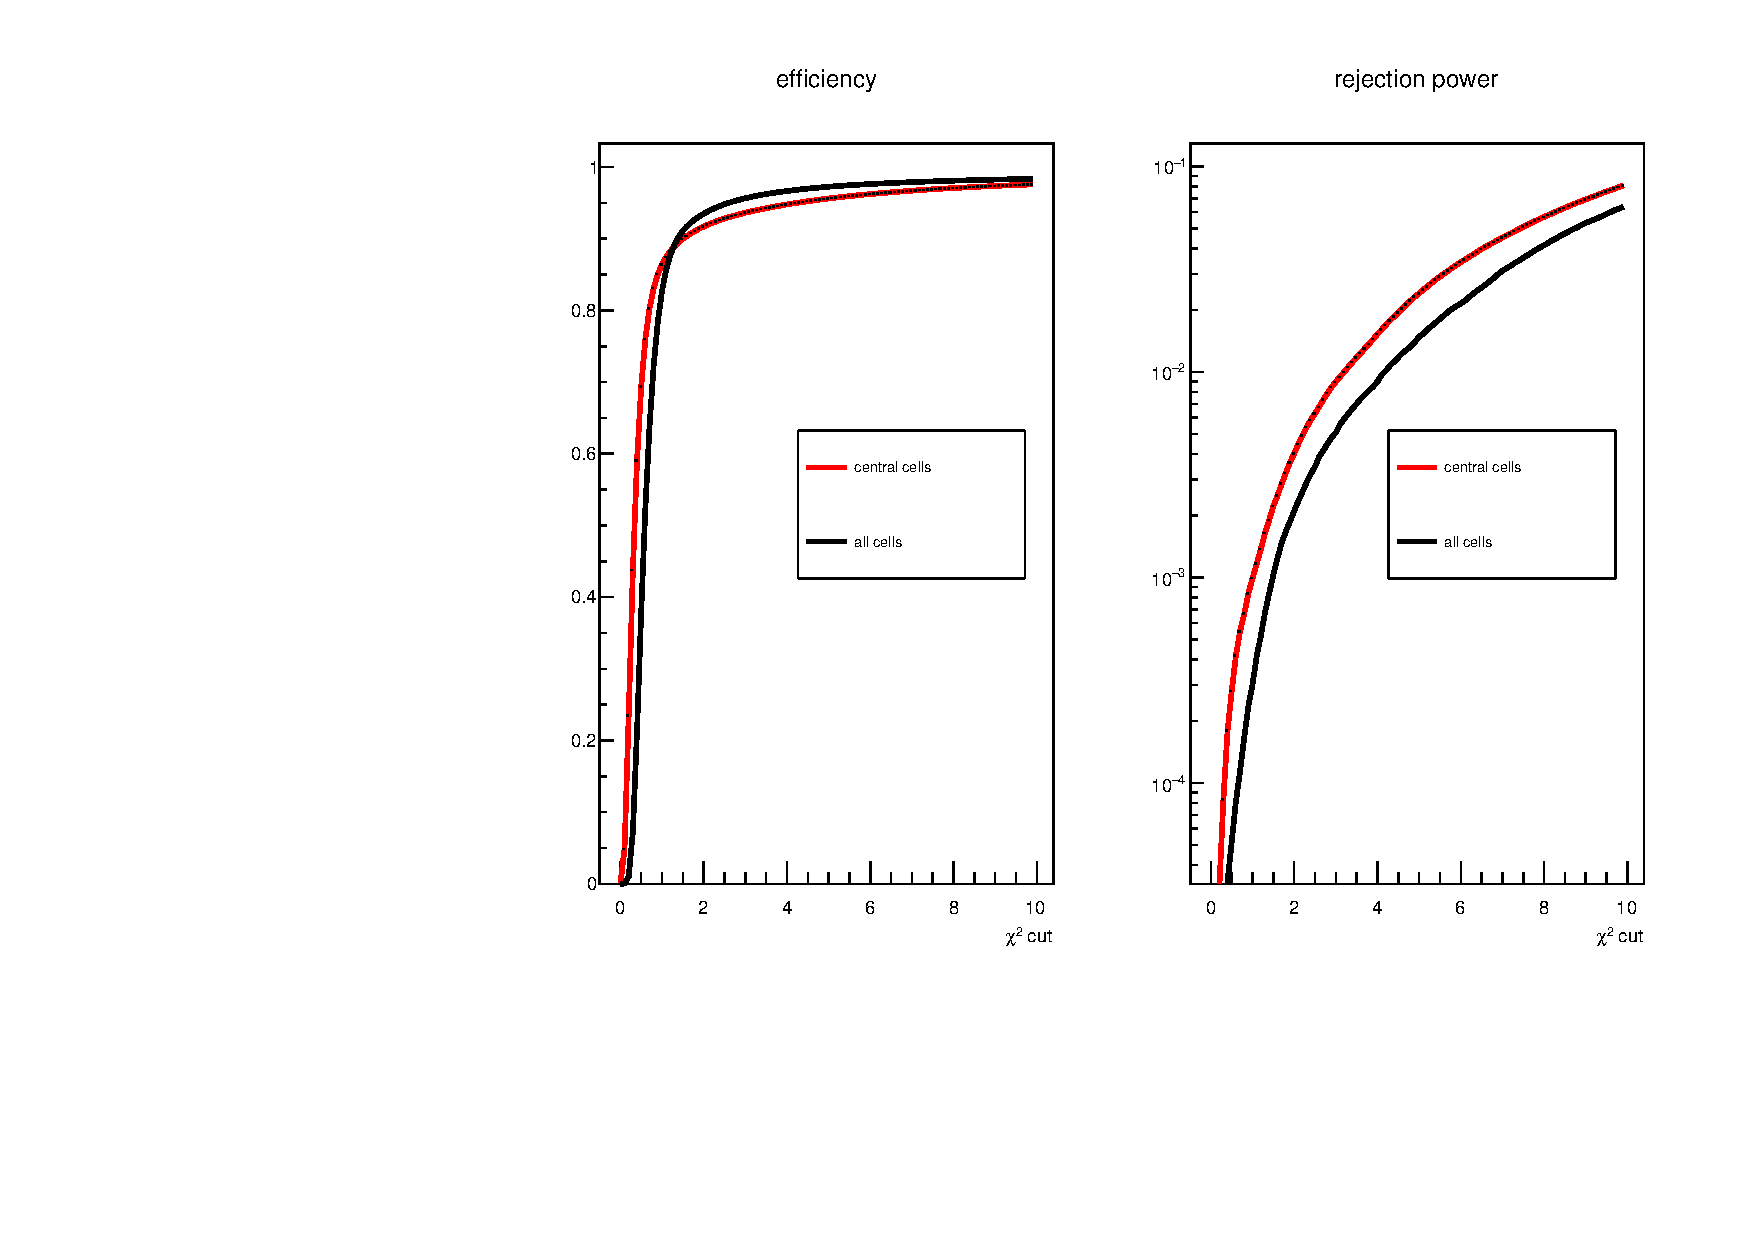
\includegraphics[width=0.95\textwidth,height=0.6\textwidth]{\pdirthree/eff.pdf}
  \end{center}
  \caption[Fraction of events passing the $\chi^2$ cut]{Fraction of events passing the cut $\chi^2 < \chi^2_{cut}$
    for the electron calibration run (left) and for the hadron calibration run (right).}
  \label{fig:eff}
\end{figure}

Different ECAL vs HCAL plots were produced to study the effect of a
$\chi^2$-cut for the run mentioned above. The one produced with
a benchmark cut of $\chi^2 < 2$ are shown in
Fig.\ref{fig:ehcal_test}. The cut is shown to clean the plot in the
way expected from the hadronic activity in all selected runs. It can also be seen from the run recorded with the physical trigger that events involving the dimuon
production $e^- \to \mu^+\mu^-$ survive the cut for energies larger
than 20 GeV.  This is expected since these events will still involve
an electromagnetic shower truncated at the moment the transition
happens. Since a possible signal from a Dark Photon would behave
similarly this suggests that the cut won't reject the signal provided
that the shower has enough energy. A similar study performed with the
MC reached the same conclusion, however, for small energy deposits the shower shape will slowly reach each cell's energy resolution and the efficiency of the cut will drop
substantially. The efficiency for low energy improves if only central
cells are selected for the $\chi^2$ calculation since this will reduce
the fluctuation of the single cells not involved in the shower. This
effect is shown in Fig.\ref{fig:ehcal_comp} for a cut of 2 on $\chi^2$.
\\
\\
For low energy particles, it is clear that all the shower will be
contained in the cell 3x3. Below this threshold shower analysis can no
longer resolve the type of shower of the event and instead the simple
requirement of the full energy of the event to be detected by the
central cell (3x3) should be used to avoid rejecting signal events. Applying a $\chi^2$-cut to a dark photon simulation suggested that this limit is roughly 5 GeV.  The left plot in Fig.\ref{fig:ehcal_comp} is compatible with this estimate.

\begin{figure}[h!]
  \begin{center}
    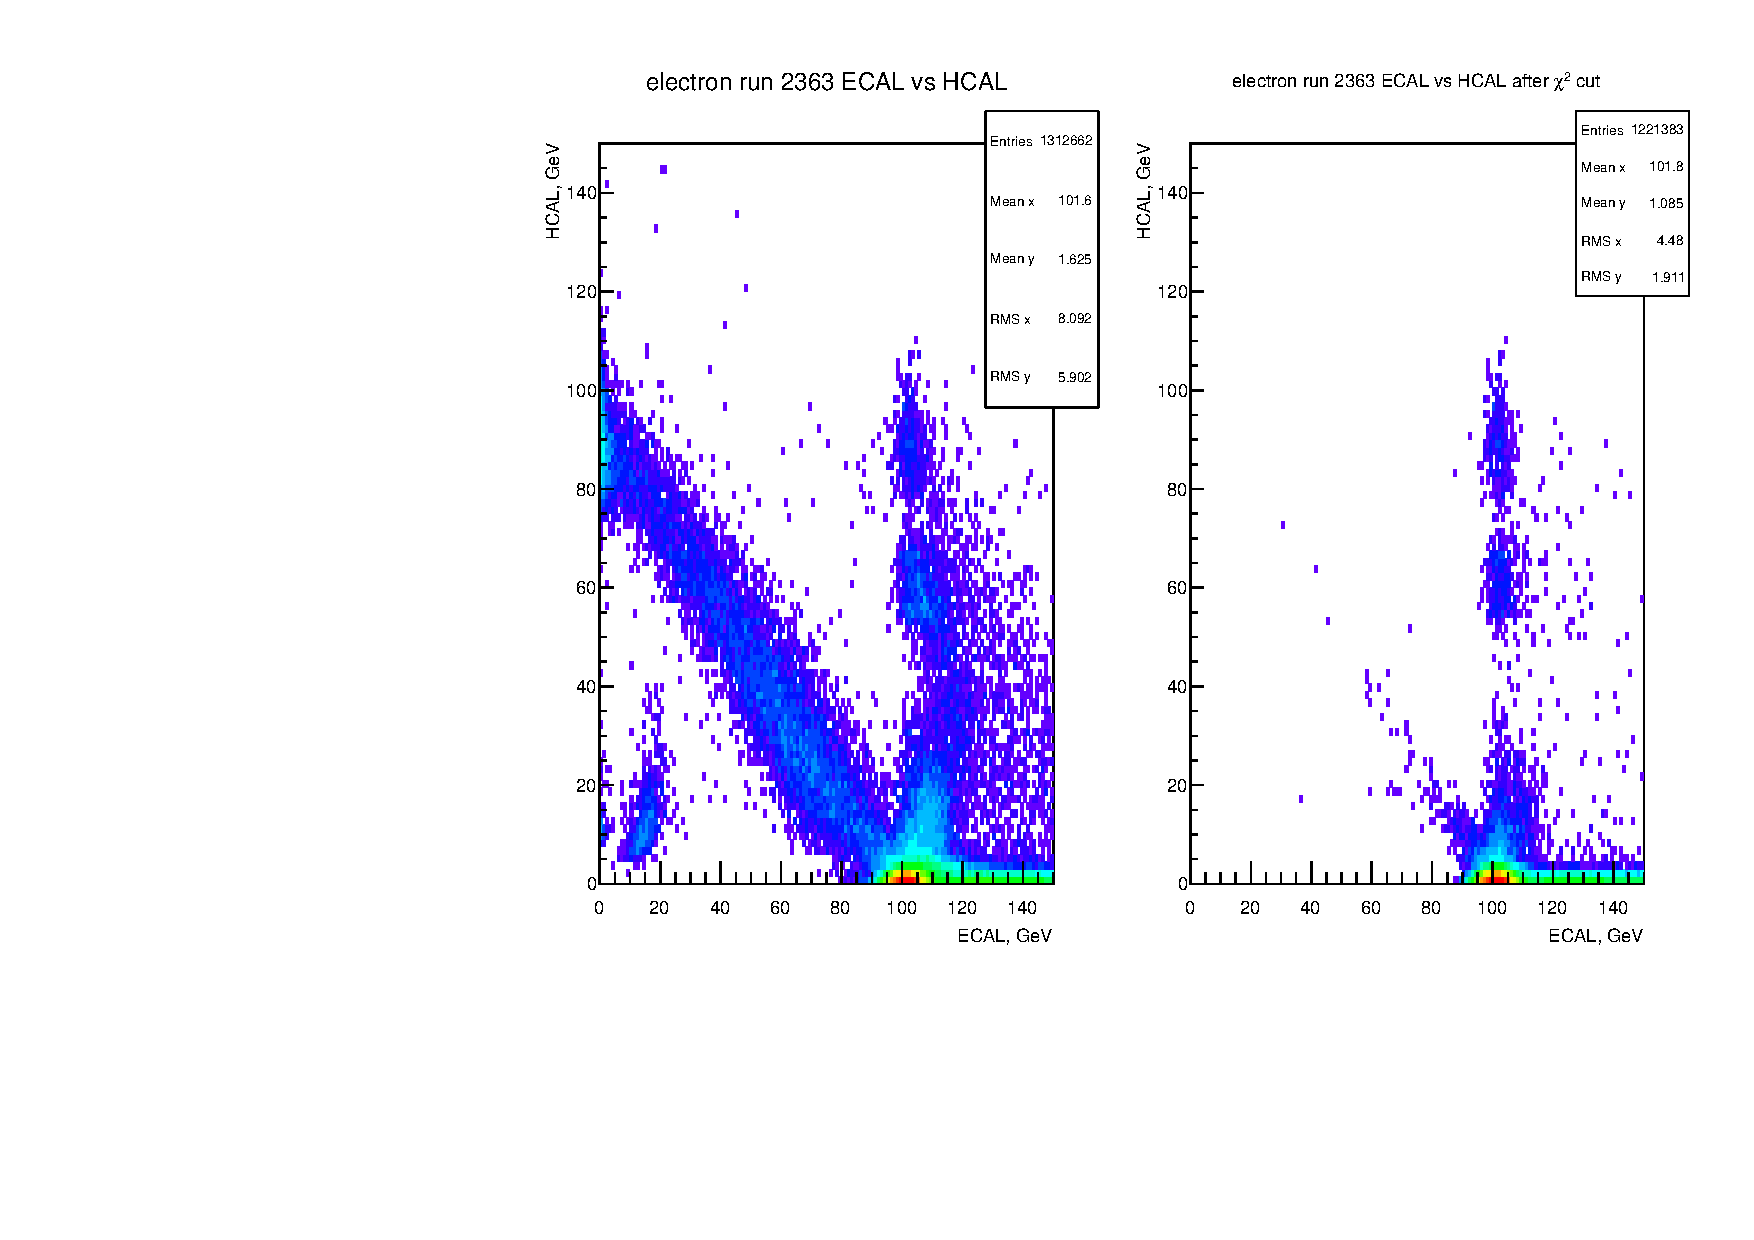
\includegraphics[width=\textwidth]{\pdirthree/ehcal_2336_chi.pdf}
    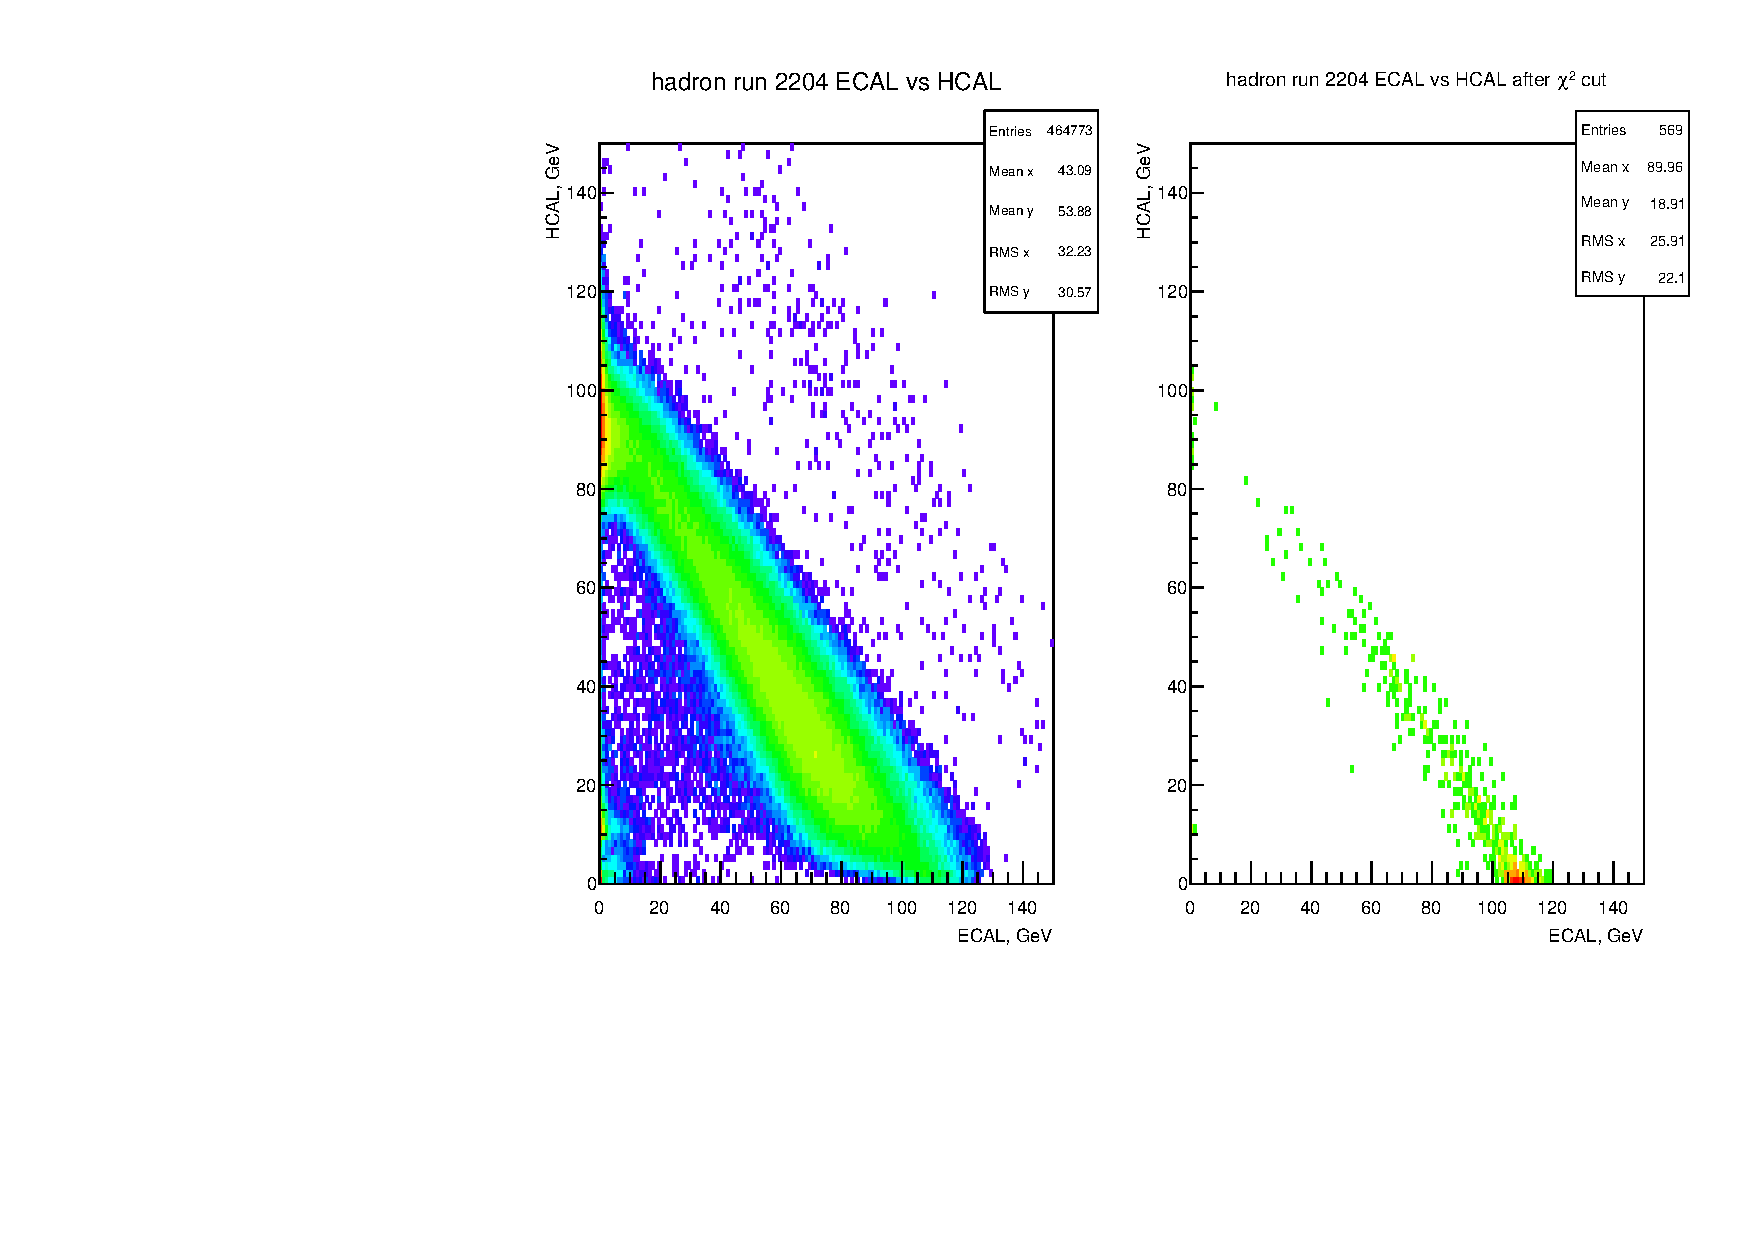
\includegraphics[width=\textwidth]{\pdirthree/ehcal_2204_chi.pdf}
  \end{center}
  \caption[ECAL vs HCAL energy deposit after a cut $\chi^2$]{ECAL vs HCAL energy deposit for the total sample (left
    column) and after a cut $\chi^2<2$ (right column) for the
    electron calibration run (top) and the hadron calibration run (bottom).}
  \label{fig:ehcal_test}
\end{figure}
\clearpage

\begin{figure}[h!]
  \begin{center}
    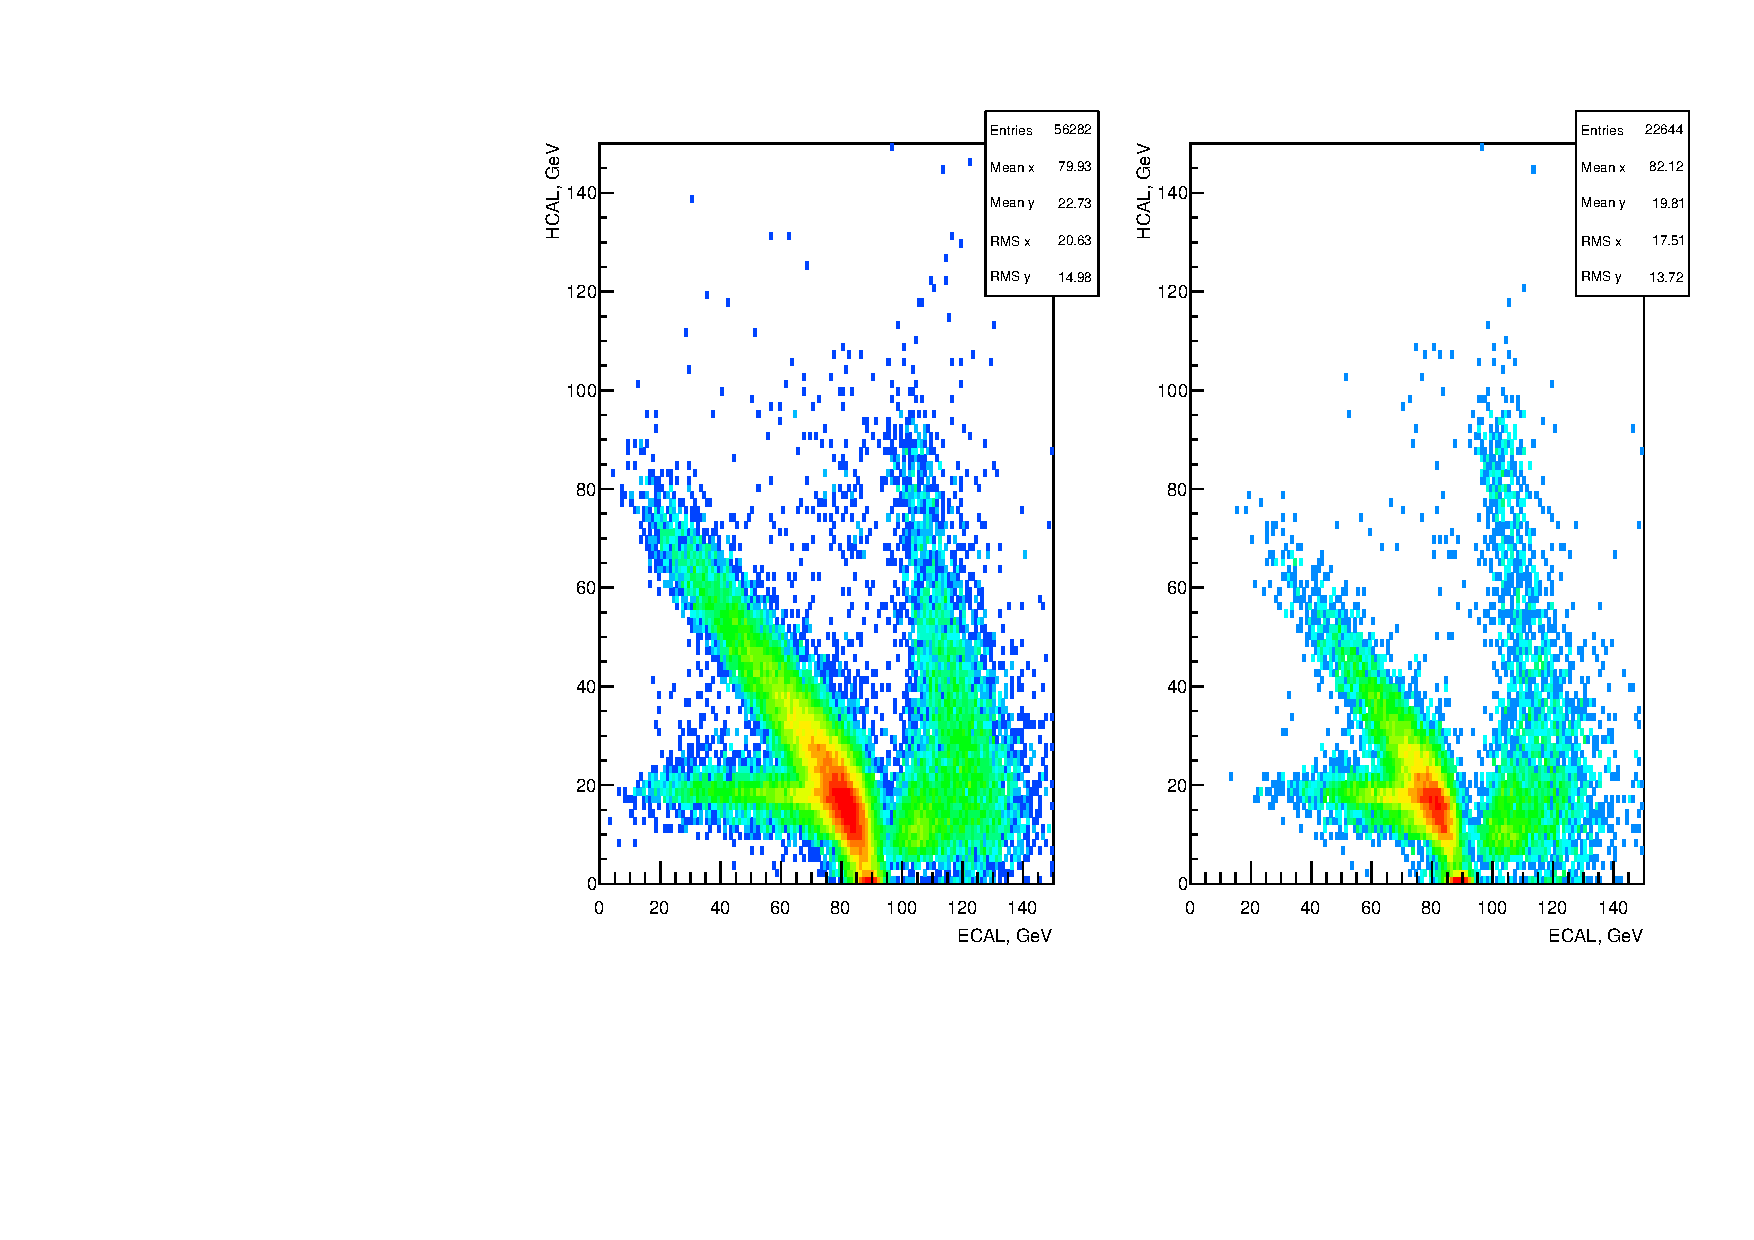
\includegraphics[width=\textwidth]{\pdirthree/ehcal_2441_comp.pdf}
  \end{center}
  \caption[ECAL vs HCAL energy deposit after a cut $\chi^2$ for different ECAL configurations]{ECAL vs HCAL in run using a physical trigger after a cut $\chi^2<2$ is applied with the $\chi^2$ calculated with the 9 central cells (left) and for all cells (right).}
  \label{fig:ehcal_comp}
\end{figure}

\section{Invisible mode analysis}
\label{ch3:sec:analysis-invis}

The general analysis method described in Sec.\ref{ch3:sec:analysis-approach} is now applied to the specific case of the invisible mode data. To apply the method a set of selection criteria is set to maximize the overall sensitivity of the setup using the MC-simulation described in Sec.\ref{ch3:sec:geant4}. The background is also detailed using the classification defined at the beginning of this chapter. We will show that the expected number of events in the signal region in absence of Dark Photon production is $\simeq 0.5$, making NA64 a background-free experiment.

\subsection{Selection criteria}
\label{ch3:sec:selection-criteria}

The cuts used are chosen based on their significance in the MC simulation, defined as:

\begin{equation}
  \label{eq:significance}
  S = \frac{s}{\sqrt{s + b}}
\end{equation}

In this context, the signal is not necessarily an event with $\DMM$ production, but the particle that the cut is supposed to select.
In the case of SRD for example, the cut is required to select electrons and reject any other kind of particle. So $s$ will be the number of electrons selected by the cut and $b$ will be the number of non-electron ($\pi^-$, $\mu^-$) selected. Since only $e^{-}$ can trigger the reaction $\ea$, this requirement also maximizes the sensitivity of the experiment. The cuts are then optimized using the calibration run and control sample to take into account the effect caused by pileup and electronics as explained in Sec.\ref{ch3:sec:analysis-approach}.

The selection criteria need to select 100 $\gev$ electrons and reject any events interacting before the target.
To achieve this the following requirements are applied:

\begin{itemize}
\item The difference between the reconstructed momentum and the nominal 100 $\gev$ beam energy is not larger than 5 $\gev$. Additionally, the entrance angle of the particle needs to be within 2 $\mrad$. The track also needs to be reconstructed with a $\chi^2<5$.
\item An energy deposit between 1.3 $\mev$ and 80 $\mev$ is required in each SRD crystal. Each signal needs to be in a time coincidence of 5 $\nas$. To reject large back-scattering from the ECAL, the maximum energy of 120 $\mev$ is allowed in total in the SRD.
\item The energy deposited in the ECAL in time with $S_0$ within 13 \nas. If more than 30 $\gev$ energy is recorded out of time, the event is rejected. Furthermore, the largest ECAL energy deposit needs to be in the central cell\footnote{The cell is labeled (3$\times$3), a sketch can be seen in Fig.\ref{fig:ecal_example}}, aligned with the beam center. 
\item Since most of the energy of an em-shower will be deposited inside the Moliere radius, the energy deposited outside the $3\times3$ matrix is required to be below 5\% of the total energy deposited. 
\item The compatibility with an em-shower is checked using the method described in Sec.\ref{ch3:sec:bkg-ecal-profile} with a $\chi^2 < 8$ cut.
\item All events with signal above noise in the VETO are rejected to avoid punch-through from the main target. The exact value of the cut is $E_{VETO} <$0.9$\times \emip$.
\item Events where the energy deposited in one of the HCAL periphery cells is larger than the one deposited in the center are rejected. This is defined using the $R$-value (see Eq.\ref{eq:R-factor}) for a cut of $R < 0.05$.
\item Events with multiple hits in the straw chamber are removed from the analysis. This cut is used to remove the contamination due to electron-hadron production upstream of the ECAL.
\end{itemize}

Finally, the signal region is defined by events with significant missing energy in the ECAL and no activity in the HCAL. This means $E_{ECAL} < 50$ $\gev$ and $E_{HCAL} < 1$ $\gev$, previously illustrated in Fig.\ref{fig:two-signature}.

The efficiency of the cuts listed above was studied using the MC simulation and the electron calibration runs.
In Fig.\ref{fig:inv-cut-ehcal} the effect of these cuts in the $\ehcalplane$ plane is shown.
The amount of hadrons is seen to be greatly reduced after the SRD cut is applied, and consequentially the dimuon region becomes more visible. The VETO cut then removes most of the punch-through particles, including dimuons. Finally, after the tracking selection, a large portion of the low energy deposit event and strong scattering upstream disappear\footnote{This is mostly visible in the requirement of "GoodTrack", visible between plots 5 and 6}.


\begin{figure}[bth!]
  \centering
   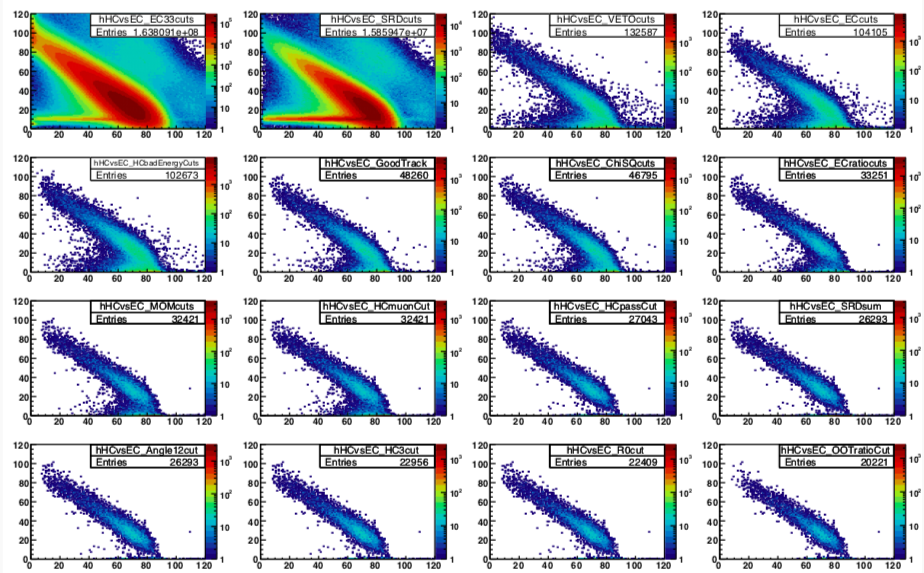
\includegraphics[width=\textwidth]{\pdirthree/ec-hc-plots-veto-nobad-runs.png}
  \caption[Effect of the cuts in invisible mode]{Selection criteria effects in the $\ehcalplane$ on the 2018 invisible mode data sample \cite{invis-cut-plot,NA64:2019imj}.}
  \label{fig:inv-cut-ehcal}
\end{figure}

\subsection{Background}
\label{ch3:sec:bkg:inv}

In this section, what constitutes background in invisible mode setup will be detailed, following the classification defined in Sec.\ref{ch3:sec:analysis-approach}. A complete summary of the expected background is provided in Table \ref{tab:inv-bkg}.
\subsubsection{Hadronic background}
\label{ch3:sec:bkg:inv:hadr}


In the case of invisible mode, the background can arise from a $\pi^-$ that travels through the HCAL undetected after leaving minimal energy in the ECAL. The probability of this happening with a total interaction length of 21 $\lambda_{int}$ is $p\lesssim 10^{-9}$ (estimated punch-through probabilities are provided in Table \ref{tab:hadron-punch-prob} for different hadron species). This number does not account for the high-efficiency VETO after the ECAL, SRD rejection, and the fact that the HCAL can detect a MIP interaction even in the absence of strong interaction. Each of these factors pushes the background well below $<10^{-13}$ as pointed out in the NA64 first proposal \cite{Andreas:2013lya}.

A more significant background is caused by the inelastic scattering inside the ECAL in a process:

\begin{equation}
  \label{eq:pion-nucleus-scattering}
  h + Z \longrightarrow h + Z + (hadrons)
\end{equation}

Part of the energy can evaporate as a consequence of some particles emitted at a large angle and thus escaping the setup in the direction transverse to the beam. This background is suppressed by shower profile analysis, energy deposited in the pre-shower, and the VETO cut. The phase space of this process is however complicated, and a lot of possible phenomenological scenarios can arise from it. For example, large energy deposited in the pre-shower can be a simple consequence of some $\pi^0$ backscattering after the hadronization. The hadron shower profile can also mimic the one of an electron if a large fraction of energy in the inelastic scattering is carried away by $\pi^0$. Also, if there is neutral particle emission such as neutrons or $\ks$, the VETO would be ineffective to reject them.

To have an estimate, we can take the process \ref{eq:pion-nucleus-scattering} and assume $\geq$2 neutral particles are produced in the hadronization. This gives us a probability equal to \cite{gkkk1}:

\begin{equation}
  \label{eq:transverse-leak-estimate}
  P \simeq P_n \cdot P_{la} \cdot P_{leak}
\end{equation}

Where $P_n$ is the probability of such interaction to occur, $P_{la}$ the one to produce particles at a large scattering angle, and $P_{leak}$ the probability to escape HCAL without interactions. Here we stress again that this formula hides a large number of topologies that such an event could have, but gives an intuition for these processes. Since the ECAL has $\lambda_{int} \simeq 0.5$, the probability of interaction is fairly high (roughly 50\%). We need at least 50 $\gev$ energy leaking to produce a signal event. If two neutrals are produced at $\Theta_{n} \simeq 30$\si{\degree} this would mean crossing at least 4$\lambda_{int}$ each, for a $P_{leak} \lesssim 3 \cdot 10^{-4}$. We can take the measured values of NOMAD to estimate the value of the cross-section in this range \cite{AUTIERO1998285,GNINENKO1998583}. The measured probability of separating a cluster with energy $>$0.1E$_{\pi}$ at an angle $\Theta_{n} \gtrsim 30$\si{\degree} is P$_{la} \simeq 10^{-5}$, dropping very quickly with the beam energy: a factor 20 difference was found between 15 $\gev$ and 6 $\gev$ $\pi^-$. Even if we take this conservative value as $P_{la}$, the probability of the energy to escape is already $P\simeq 10^{-9}$, which multiplied to the hadron contamination and SRD suppression leads to an estimate of $P<10^{-14}$ for this background.

Another possible background is the decay of hadron inside the setup in neutrinos, which would cause some energy to disappear from the setup. The high-energy of the primary suppress this background, since at 100 GeV the chance for a $\pi^-/K^-$ to decay is $P^{decay}_{\pi} \simeq  10^{-2}$. Multiple possible decays are accompanied by a neutrino emission, the most likely one being $\pi^- \rightarrow \mu^- +\nu_{\mu}$. The emission of the muon makes such decay very easy to spot since it will leave an energy deposit both in the VETO and the HCAL, for a total probability similar to the one of a punch-through $\pi^-$ ($P < 10^{-14}$). One could argue that the $\mu^-$ could decay: $\mu^- \rightarrow e^- + \nu_{\mu}+ \bar{\nu_{e}}$, producing an electromagnetic shower with missing energy. The long decay time of the $\mu^-$ adds however an additional suppression factor of $P\simeq 10^{-5}$, which together with the upstream selection criteria put the background conservatively at $P \lesssim 10^{-13}$.

Another background comes from the decay $K^- \rightarrow \pi^0 + e^- + \bar{\nu_e}$, commonly called $K^-_{3e}$, with a branching ratio of $\Gamma_i/\Gamma_{tot} \approx$0.05 \cite{particle-strange-mesons}. The total probability of background for an incoming $K^-$ is around $P\simeq 10^{-3}$, accounting for both probabilities of decaying and the branching ratio of $K^-_{3e}$. A MC-simulation of $K^-$ confirms this estimate as shown in Fig.\ref{fig:kaonbkg-sim}, where the fraction of the events in the signal region corresponds to the probability calculated. 
Multiplying this probability for the SRD selection criteria and the beam suppression returns a value of $P_{K_{3e}} < 10^{-12}$.
There are however additional factors of rejection for this background that can be investigated using simulations. A precise account of all cuts in the MC shows push this background to $P_{K_{3e}} \lesssim 10^{-13}$.


\begin{figure}[bth!]
  \centering
  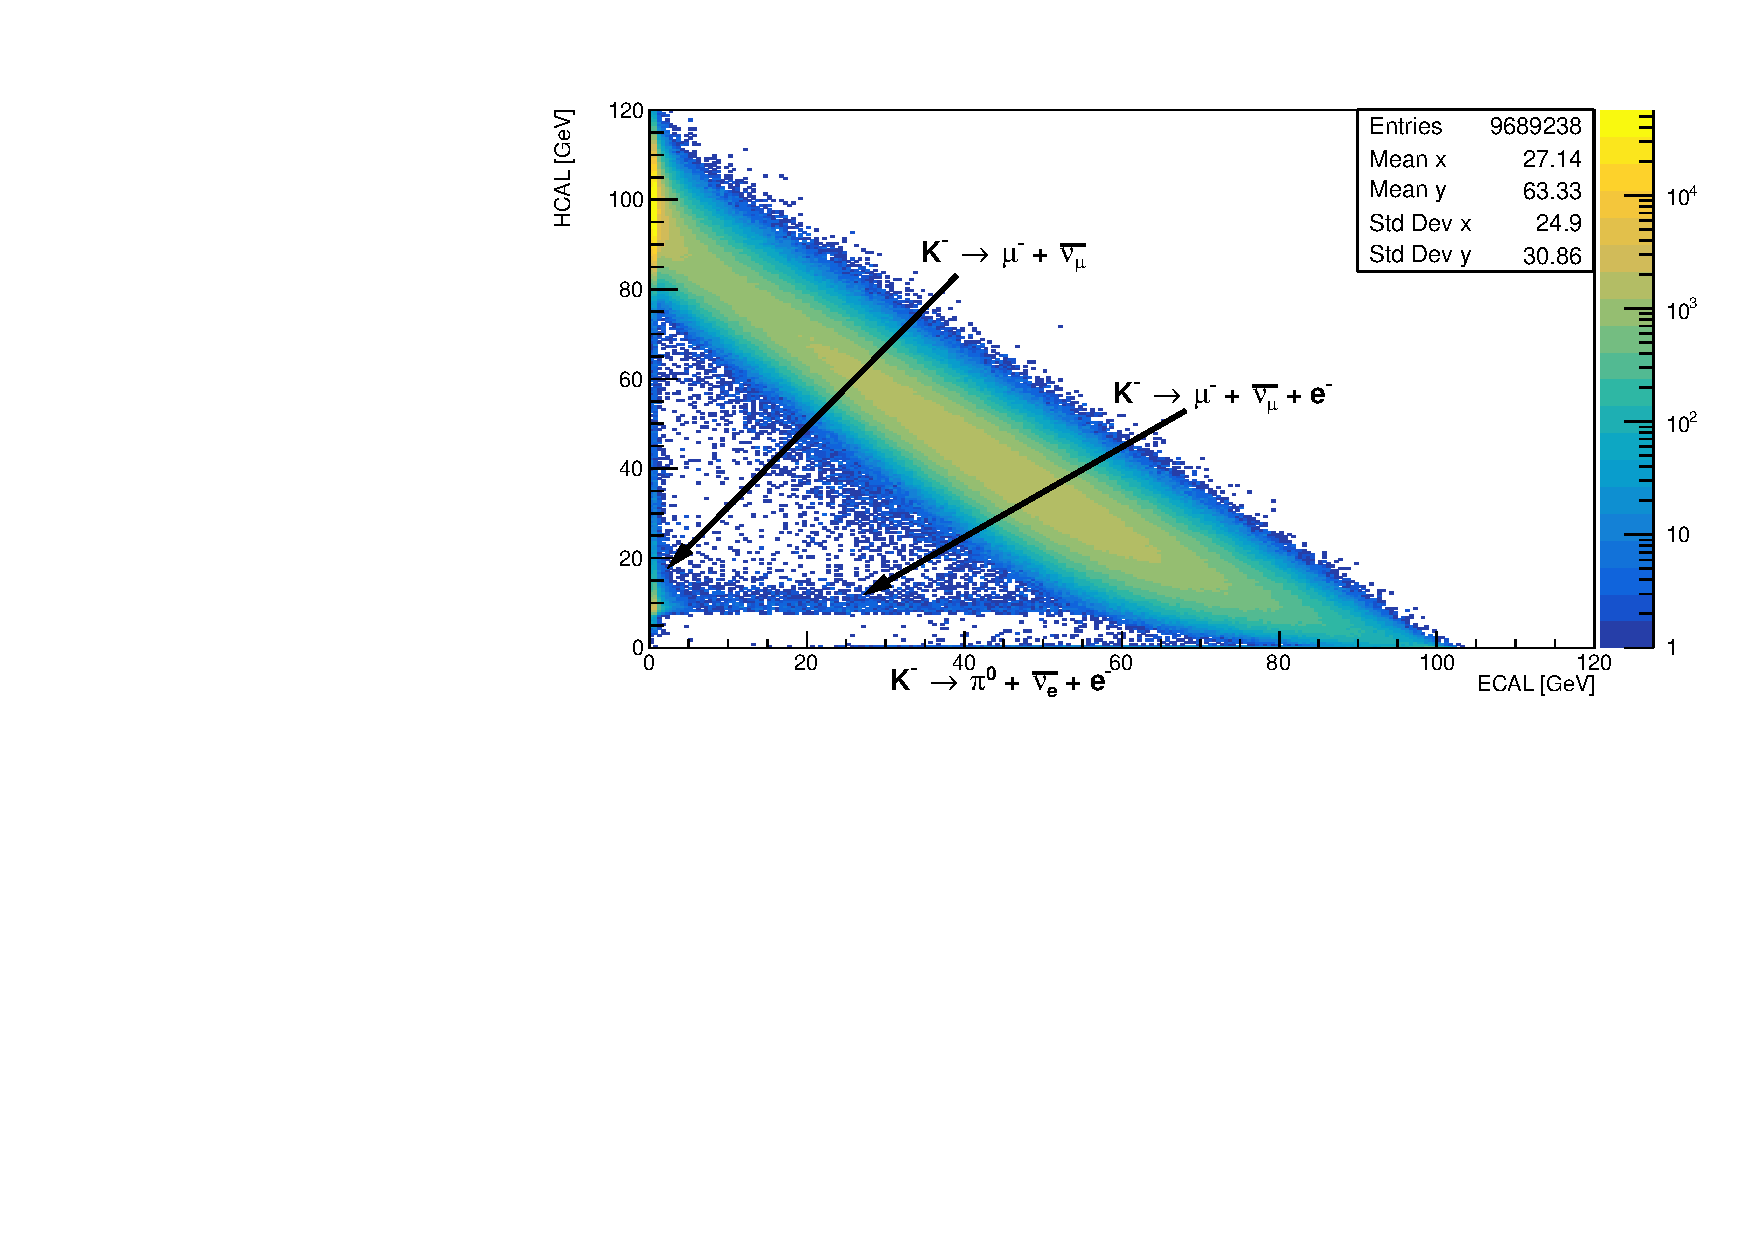
\includegraphics[width=\textwidth]{\pdirthree/kaonbkg.pdf}
  \caption[$K^-$ simulation ]{Energy deposited in the $\ehcalplane$ plane after simulating $10^7$ $K^-$ as primary particle in the NA64 setup.}
  \label{fig:kaonbkg-sim}
\end{figure}

\subsubsection{Muonic background}
\label{ch3:sec:bkg:inv:muon}

This type of background is also largely suppressed by both beam composition and SRD selection criteria, to a level of $\lesssim 10^{-7}$. As in the case of $\pi^-$, a complete punch-through of the setup without being detected is negligible. Indeed the muon needs to travel through both the VETO and the three HCAL modules without leaving any detectable energy deposit. These probabilities are $p^{VETO} \simeq 10^{-3}$ for the VETO and $p^{HCAL} \simeq 10^{-4}$ for the HCAL case resulting in a background $< 10^{-14}$.
In the case of muons, nuclear interaction is less likely. Thus, there is no possibility that a large fraction of energy escapes transversely. 
What remains is the decay $\mu^- \rightarrow e\nu\nu$, with neutrinos in the final state. The decay time of $\mu^-$ adds a suppression of $\lesssim 10^{-5}$. Similar to the previous case, SRD selection, tracking, and shower profile account for an additional $p\sim 0.1$ factor. This background level is of $P_{\mu} \lesssim 10^{-13}$.

\subsubsection{Electronic background}
\label{ch3:sec:bkg:inv:elec}

Since the beam is primarily made of electrons, and SRD is tuned to select them, no upstream suppression factor can be achieved in this case. Simple punch-through of an electron through the whole setup is not possible, since the path is blocked by 3 HCAL modules. Other similar events, with energy losses due to non-uniformity and cracks in the ECAL/HCAL were as well studied and found unrealistic \cite{Andreas:2013lya}. Low energy electrons a potential source of background: if a primary electron with $E_0 < E_{th}$ arrives at the ECAL it will leave an energy deposit compatible with the signal. Such a background was also found extremely unlikely. The amount of electron $N(E_e<E_{th})$ in the beam with energy lower than the energy threshold for the signal amounts conservatively to $<10^{-2}$. Such particles are normally deflected by the two MBPL magnets outside the acceptance of the ECAL\footnote{For $E_0$=50 $\gev$ the difference in deviation is about 0.4 \si{\meter}}. Particles with large entrance angle in the magnet are still capable of hitting the ECAL, but the tracking system makes sure that their energy is reconstructed with a resolution of $\delta p/p \approx 1\%$ \cite{Banerjee:2017mdu}. A dedicated simulation of $10^{10}$ electrons with energy compatible with the signal region was performed. No signal-like event was found after requiring a reconstructed momentum of 100 $\gev$ with a tolerance of 3$\sigma$. Extrapolation to the signal region of the spectrum put this background level at $\lesssim 10^{-13}$.

An important source of background to be considered is the dimuon production inside the target. As mentioned, these events are very useful to check for systematics and validate the MC. However, fluctuations in the energy deposited in the HCAL might leak in the signal region. The background was estimated by exponential extrapolation of the control sample inside the signal region ($E_{HCAL} < 1 \gev$) considering the sideband I depicted in Fig.\ref{fig:ehcal-bkg-bands}. The VETO cut was not applied to the control sample for this extrapolation and was accounted separately as a factor $\sim 10^{-6}$ (probability of two MIPs to leave no energy).

\begin{figure}[bth!]
  \centering
  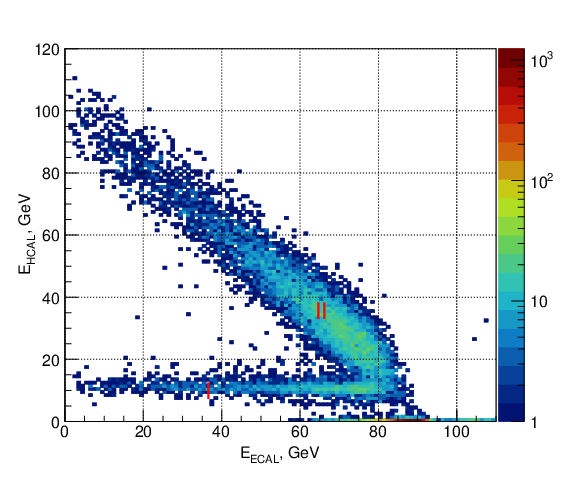
\includegraphics[width=0.45\textwidth]{\pdirthree/EHCAL_lastpub_left.png}
  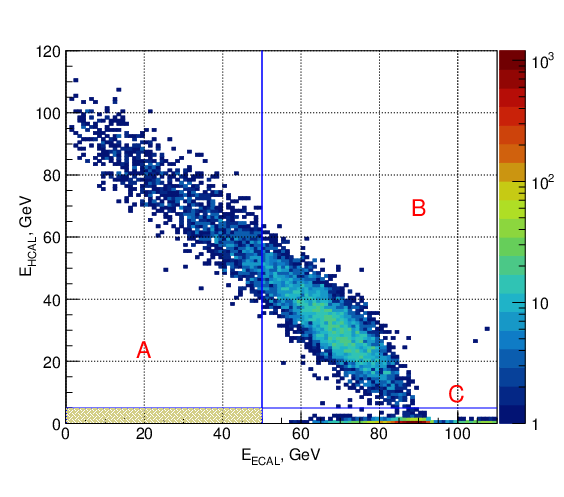
\includegraphics[width=0.45\textwidth]{\pdirthree/EHCAL_lastpub_right.png}
  \caption[ECAL vs HCAL events band]{Distribution of events in the $\ehcalplane$ plane for the data control sample. The right panel shows the sample with all the selection criteria. The left panel shows the same sample without the VETO cut. The shaded area is the signal box. The size of the signal box is increased by a factor 5 in the Y-axis direction for illustration purposes. The region labeled I contains events caused by dimuon production, while region II contains mostly events leaking from the ECAL into the HCAL. The sidebands A and C are used to estimate the background inside the signal region \cite{NA64:2019imj}.}
  \label{fig:ehcal-bkg-bands}
\end{figure}

Finally, the leading background in the invisible mode setup is the electro-nuclear and photo-nuclear production of neutral hadrons at a large angle. This case is similar to the one discussed for hadrons, but no additional suppression due to beam-composition and SRD selection criteria is present. In first approximation, the rarity of such interaction balances the absence of suppression factors, and accounts for $P_n \simeq 10^{-6}$ (see Eq.\ref{eq:transverse-leak-estimate}).
The largest source of background, however, comes from electro-nuclear production happening upstream of the target. As Fig.\ref{fig:eh-prod-sketch} shows, if this interaction happens in a detector at a large distance from the ECAL, the deviation of the particle can be large enough to exit the setup transversely. 


\begin{figure}[bth!]
  \centering
  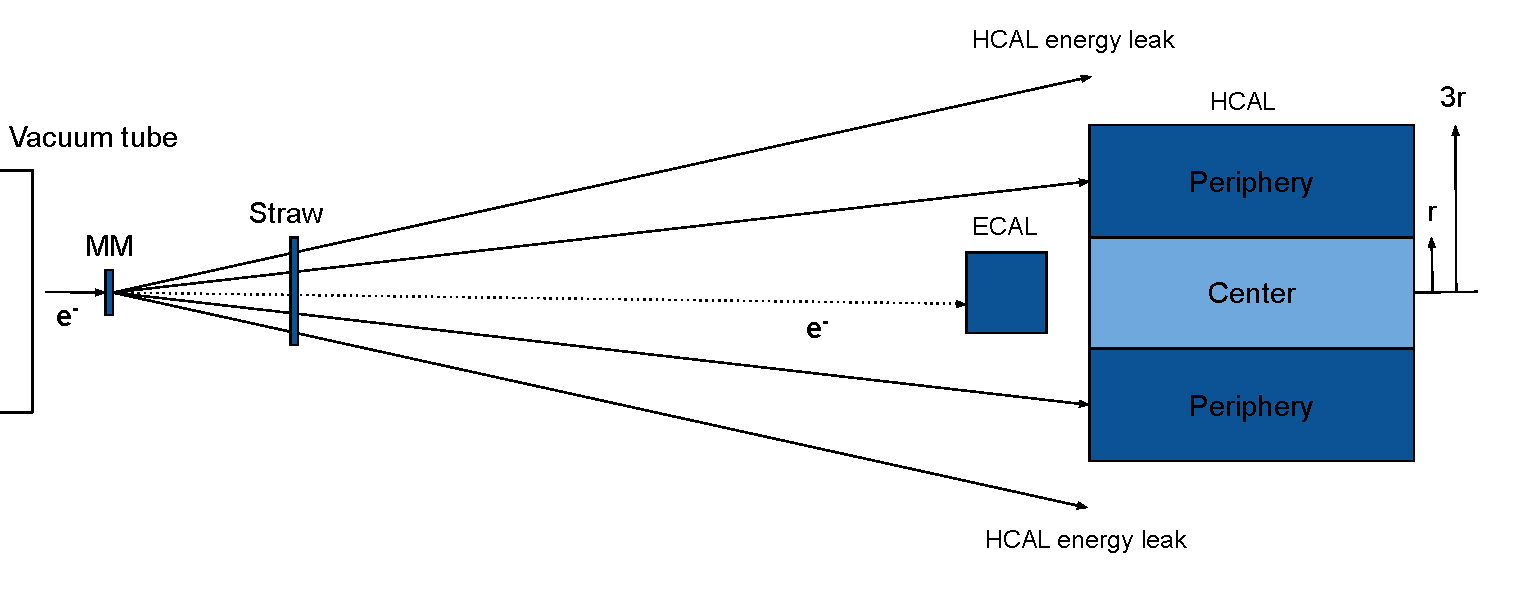
\includegraphics[scale=0.4]{\pdirthree/hcal-leak.pdf}
  \caption[upstream electro-hadron production upstream]{Sketch of electro-nuclear interaction happening upstream the ECAL leading to a possible background \cite{pdegen-thesis}.}
  \label{fig:eh-prod-sketch}
\end{figure}

This background can be estimated by looking at the periphery region of the HCAL. Since the angular distribution is sharply suppressed for large angle \cite{AUTIERO1998285,GNINENKO1998583}, these particles typically leave an energy signature in the periphery of the first HCAL when they miss the ECAL. To characterize this, we define the variable $R$ as the ratio between energy deposited in all cells excluding the central one, and the total energy deposited in the modules:

\begin{equation}
  \label{eq:R-factor}
  R = \frac{E^{all}_{HCAL} - E^{center}_{HCAL}}{ECAL^{all}_{HCAL}}
\end{equation}

In a standard event with particles leaking the ECAL the largest HCAL energy deposit will be in the central cell as it is aligned with the beam direction. The typically observed value for those events will be $R<0.5$.
However, If an electro-nuclear production happens upstream, some distortion of this variable will be visible. In the most extreme scenario when the particle is missing the ECAL completely, the $R$ value will be equal 1, since the central cell of the HCAL will be shielded by the ECAL while the periphery will be directly hit. We can observe such behavior in Fig.\ref{fig:r-value-csample}: most of the events considered have an $R$ peaked at 0.35. Events, where the primary electron loses a large portion of its energy due to Bremsstrahlung, are shown in region III and are responsible for events with large R. In this type of events, the electron misses the ECAL after losing energy due to Bremsstrahlung and being deflected by the magnetic field. The high-energy photon emitted propagates without being deflected and hits the HCAL in the periphery. Such events are also identifiable using the HCAL placed along the original beam direction (HCAL$_4$). In the region III, this detector measures energy deposit $E>60$ $\gev$.

\begin{figure}[bth!]
  \centering
  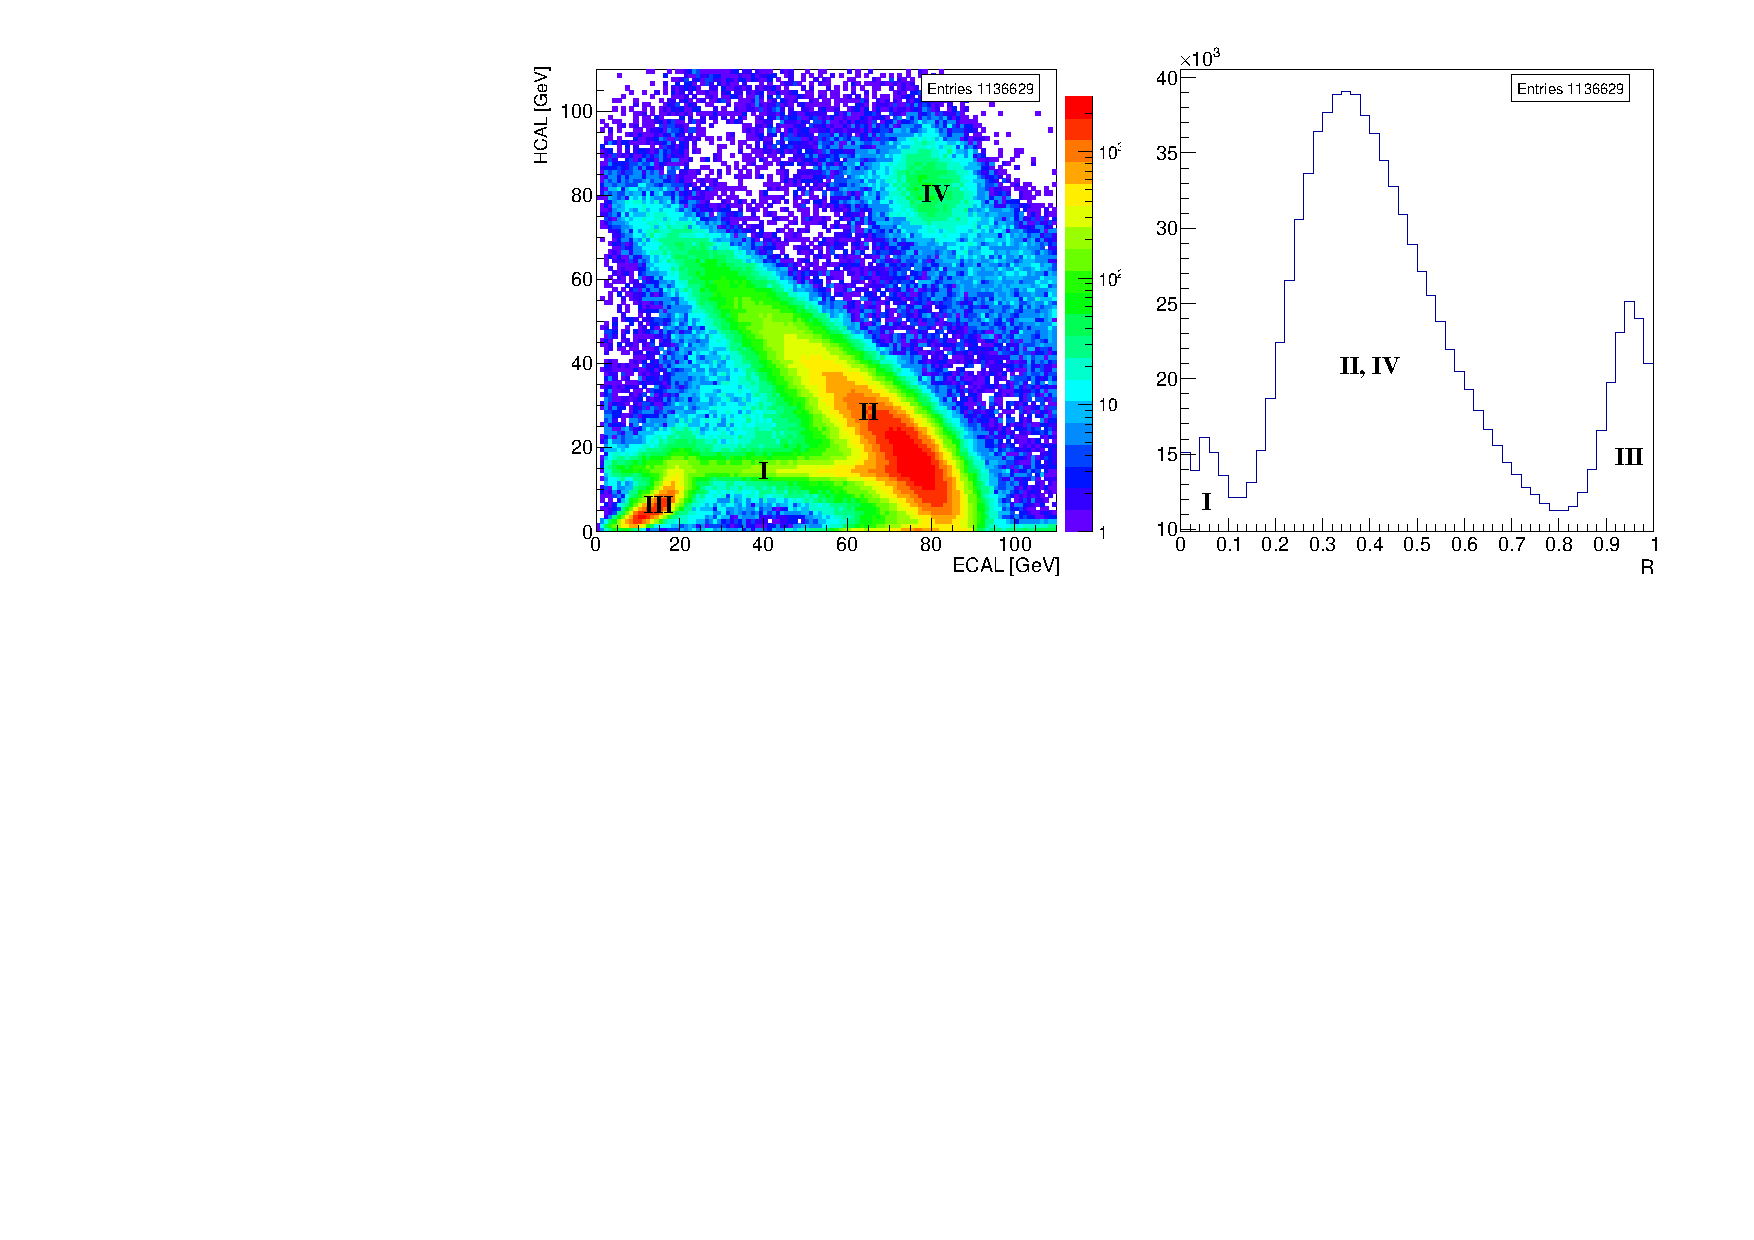
\includegraphics[width=\textwidth]{\pdirthree/pp30-calsr-uncut-may2.pdf}
  \caption[R value for the control sample]{Energy distribution in the $\ehcalplane$ (left) and the corresponding distribution of the R for different interesting regions. Region I is populated by the dimuon production inside the ECAL. Region II are events leaking in the HCAL characterized by energy conservation. Region III contains events with hard Bremsstrahlung of the $e^-$ upstream, where the primary misses the ECAL and the $\gamma$ energy is deposited in the HCAL periphery. Region IV is populated by pileup events \cite{pdegen-thesis}.}
  \label{fig:r-value-csample}
\end{figure}

Events with electro-nuclear scattering upstream are characterized by a distribution equivalent to the one of region III. The agreement of the $R$ distribution between data and simulation was checked using calibration runs, which show a good fit with the simulated samples and small differences between different hadrons species (see Fig.\ref{fig:R-comp}). This background is suppressed by two cuts:

\begin{itemize}
\item The straw tubes in the beamline, as shown in Fig.\ref{fig:eh-prod-sketch}, are in the way of the hadrons and can detect them in the periphery of their active area. A simple constraint that requires all hit to be within 3$\sigma_{beam}$ can reject this background effectively. A cut based on the multiplicity of the hit was observed to be equally powerful since electro-nuclear interaction will produce a large number of particles in the final state \cite{pdegen-thesis}.
\item Since electro-nuclear interactions produce a large number of particles, a large amount of charge is deposited on the MM strips. A cut based on the total charge measured in each plane suppresses this background efficiently \cite{na64-invisible-cuts}.
\end{itemize}

The cut on the total hits in the Straw chambers removed the contamination in the control sample and was accounted for in the final background estimate. In practice, the background was extrapolated using an exponential distribution fitted using the data in the sideband C of the control sample. The result of this estimate is shown in Table \ref{tab:inv-bkg}.

\begin{figure}[bht!]
  \centering
  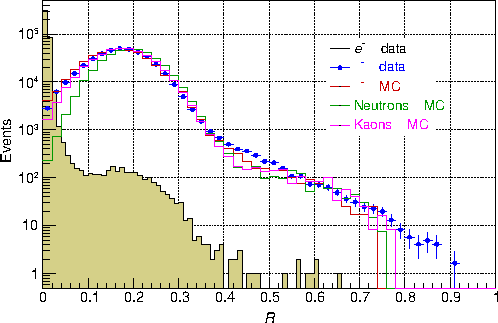
\includegraphics[width=\textwidth]{\pdirthree/HCraio-e-428-pi-3924-MC.pdf}
  \caption[R value comparison]{Distribution of the R variable for the 80 $\gev$ $e^-$, $\pi^-$, $K_L^0$ and n events obtained from data during the ECAL and HCAL calibration runs \cite{Banerjee:2020fue}.}
  \label{fig:R-comp}
\end{figure}

\begin{table}[bth!]
  \centering
  \caption[Invisible mode background]{Expected background for 2.84 $\times$ $10^{11}$ EOT collected at the time this thesis was written \cite{NA64:2019imj}}
  \begin{tabular}{lr}
    \hline \hline
    Background source & Background, $n_b$ \\
    \hline
    $\pi^-$,$\mu^-$ punchthrough                      & $<10^{-14}$ \\
    low energy $e^-$                                  & $<10^{-13}$ \\
    $e^-$/hadron nuclear interaction in target        & $<0.044$   \\
    $\pi^-$,$\mu^-$, $K_{3e}$ decay                    & 0.02 $\pm$ 0.01 \\
    $e^-$ nuclear interaction in the  beam line       & 0.43 $\pm$ 0.16 \\
    \hline
    Total (conservatively)                            & 0.53 $\pm$ 0.17 \\
    \hline \hline                       
  \end{tabular}
  \label{tab:inv-bkg}
\end{table}


\FloatBarrier\noindent
\section{Visible mode analysis}
\label{ch3:sec:analysis-vis}

An overview of the selection criteria and background specific conditions to the visible mode search is covered in this section. A new analysis performed using the 4 GEMs tracker inside the decay volume is also described. The validation of the MC and signal correction are done following the method described in Sec.\ref{ch3:sec:dimuons}, but also including a new tracking procedure developed to reconstruct vertex candidates in the decay volume. The background condition is similar for this analysis, as the selection criteria only differ for the low energy $\DMM$ produced in the late stage of the em-shower. A complete list of the expected background for both analyses is provided in Table \ref{tab:vis-bkg}.

\subsection{Selection criteria}
\label{ch3:sec:selection-criteria-vis}

For the visible mode, the signal is tagged by matching the energy deposited in the target with the one detected by the ECAL downstream. Similarly to the invisible mode, several selection criteria ensure that the incoming particle is a well-defined electron track. Although the tracking procedure is still used to work with the control sample, the incoming particle is not required to have a momentum matching the nominal beam energy. This because the signal region is already defined in a way that ensures the energy of the primary to be constraint in the same way.

The selection criteria for the visible mode can be summarized as follow:

\begin{itemize}
\item An energy above 1 $\mev$ is required in each SRD and the total energy detected in both counters needs to be larger than 10 $\mev$. Events, where the energy deposit surpasses 200 $\mev$, are removed to suppress large scattering upstream or back-scattering from the WCAL.
\item Energy deposit $E_{PS} > \SI{5}{\giga\electronvolt}$ compatible with an electron in the WCAL pre-shower.
\item At least 25 $\gev$ deposited in the ECAL. This cut rejects events where low energy particle punch-through the WCAL.
\item The maximal energy of the shower should be deposited in the ECAL cell aligned with the beam axis (labeled as 3$\times$3). 
\item The longitudinal and lateral shape of the shower should be consistent with a single em-shower\footnote{The distance of a few $\mmi$ between the two particles causes a significant overlap of the two em showers.}, $\chi^2 < 10$.
\item The energy deposited in the pre-shower compatible with a $\ee$ pair impacting the ECAL, i.e. $E_{PS} > \SI{3}{\giga\electronvolt}$.
\item VETO energy smaller than $E_{VETO} < 0.9\times \emip$, energy deposited in the HCAL smaller than $E_{HCAL}<$1 $\gev$.
\item Energy deposited in S4 compatible with two MIPs in the decay volume, using a cut $E_{S_4} > $1.5$\times \emip$.
\item  No energy deposited in the W2 counter placed after the WCAL. The value of this cut is $E_{W2} < $0.7$\times \emip$ \cite{Banerjee:2019hmi}.
\end{itemize}

The signal region corresponds to events where the sum of WCAL and ECAL energy is matching the nominal beam energy within the detectors energy resolution, i.e. $\SI{130}{\giga\electronvolt} < (E_{WCAL} + E_{ECAL}) < \SI{200}{\giga\electronvolt}$ (see Fig.\ref{fig:two-signature}). This energy was originally 100 $\gev$ in 2017 run, but was increased to 150 $\gev$ in 2018 to boost the sensitivity for short-lived $\DMX$ (see Fig.\ref{fig:w-e-vis}).

\subsection{Visible mode analysis using the tracking approach}
\label{ch3:sec:vis-mode-tracking}

The published analysis using the data collected in 2018 \cite{Banerjee:2019hmi} was based exclusively on a calorimetry approach as described in Sec.\ref{ch2:sec:vismode}. The trackers after the decay volume were not used for signal discrimination. Here we present a novel method that exploits their information providing a boost in the signal yield while maintaining the background under control. This analysis was performed by me using the GEM trackers inside the decay volume and was included in a recent article. Even though this analysis is not sensitive when the decay length of the $\DMM$ is significantly smaller than the dimension of the dump, it has the advantage of being complementary to the calorimeter analysis. It provides independent confirmation of the results obtained in \cite{Banerjee:2019hmi}, and a validation of the tracking procedure for short-lived particle searches in the next generation of this experiment (see Sec.\ref{ch5:sec:new-vismode-setup}).

While in a first approximation the $\DMM$ is produced in the first few layers of the WCAL, it can also originate at a later stage of the em-shower. These events, which are typically rejected in the calorimeter analysis, are instead accepted in the new work presented here. First, an initial sample is selected in the same way described above. The final discrimination in the calorimeter analysis is based on the counter W2 placed at the end of the dump to reject the charged punch-through from the em-shower. This last cut is efficient if the $\DMM$ is produced in the first few layers of the WCAL but typically rejects the event if the $\DMM$ is produced at a later stage of the em-shower. The reason is that these events are accompanied by a long longitudinal development of the em-shower that leaves an energy deposit larger than the typical energy cut accepted in the calorimeter analysis. On the other hand, the low energy of the produced $\DMM$ implies a larger angle between the decay products that can be resolved by the trackers. Combining these two concepts, one can see that the signal yield is characterized by two different topologies that can be distinguished by looking at the energy deposited in the ECAL (see Fig.\ref{fig:combined-analysis}).

Using this distinction, we divide all events that passed the initial selection criteria into two topologies.
The exact value of this threshold was chosen to maximize the signal yield. The optimal value has a small dependence on the $\DMM$ mass and coupling. A threshold of 75 $\gev$ amounting to half of the initial beam energy was found to be robust for most of the interesting signal scenario. After the topology is decided, a final set of cuts is applied to discriminate between signal and background. In the case of high-energy $\DMM$, trackers do not have the capability of discriminating between single hits. If the energy deposited in the ECAL exceeds 75 $\gev$, the selection criteria applied will be the one described in the previous section. On the other hand, if it is smaller, trackers are used instead of the W2 as a discriminator for an $\DMM$ production.In this case, two tracks in the decay volume were required with a reconstructed vertex within 3$\sigma$ from the WCAL and an angle smaller than 3 $\mrad$.

The different treatment increased the efficiency of the $\DMM$ produced at a late stage of the shower as shown in Fig.\ref{fig:combined-analysis}. However, the smaller energy of the $\DMM$ produced in this way reduces the probability of the particle escaping the dump. For large couplings $\epsilon$ this suppression can be more than 2 orders of magnitude, making the boost of signal yield negligible. A summary of this boost for various interesting $\DMM$ scenarios is illustrated in Table \ref{tab:dm:efftable}. The values reported consider also a correction factor of 0.77$\pm$0.1 to the signal yields that takes into account inefficiencies of the detectors and the reconstruction algorithm. This factor was evaluated using a data-driven method outlined in Sec.\ref{ch3:sec:dimuons}. We conclude that in the current setup trackers do not improve the limit on the $\DMX$ parameter space significantly. This is because the boost in signal yield becomes negligible for $\epsilon \sim 6 \times 10^{-4}$, a value which is already excluded with 90\% confidence by our previous analysis \cite{Banerjee:2019hmi}. Nevertheless, the previous results were confirmed by this independent analysis, which was also useful to outline the limitations of the current setup. This knowledge was used to design the next generation of the visible mode, as detailed in Sec.\ref{ch5:sec:new-vismode-setup}.

\begin{figure}[tbh!]
  \centering
  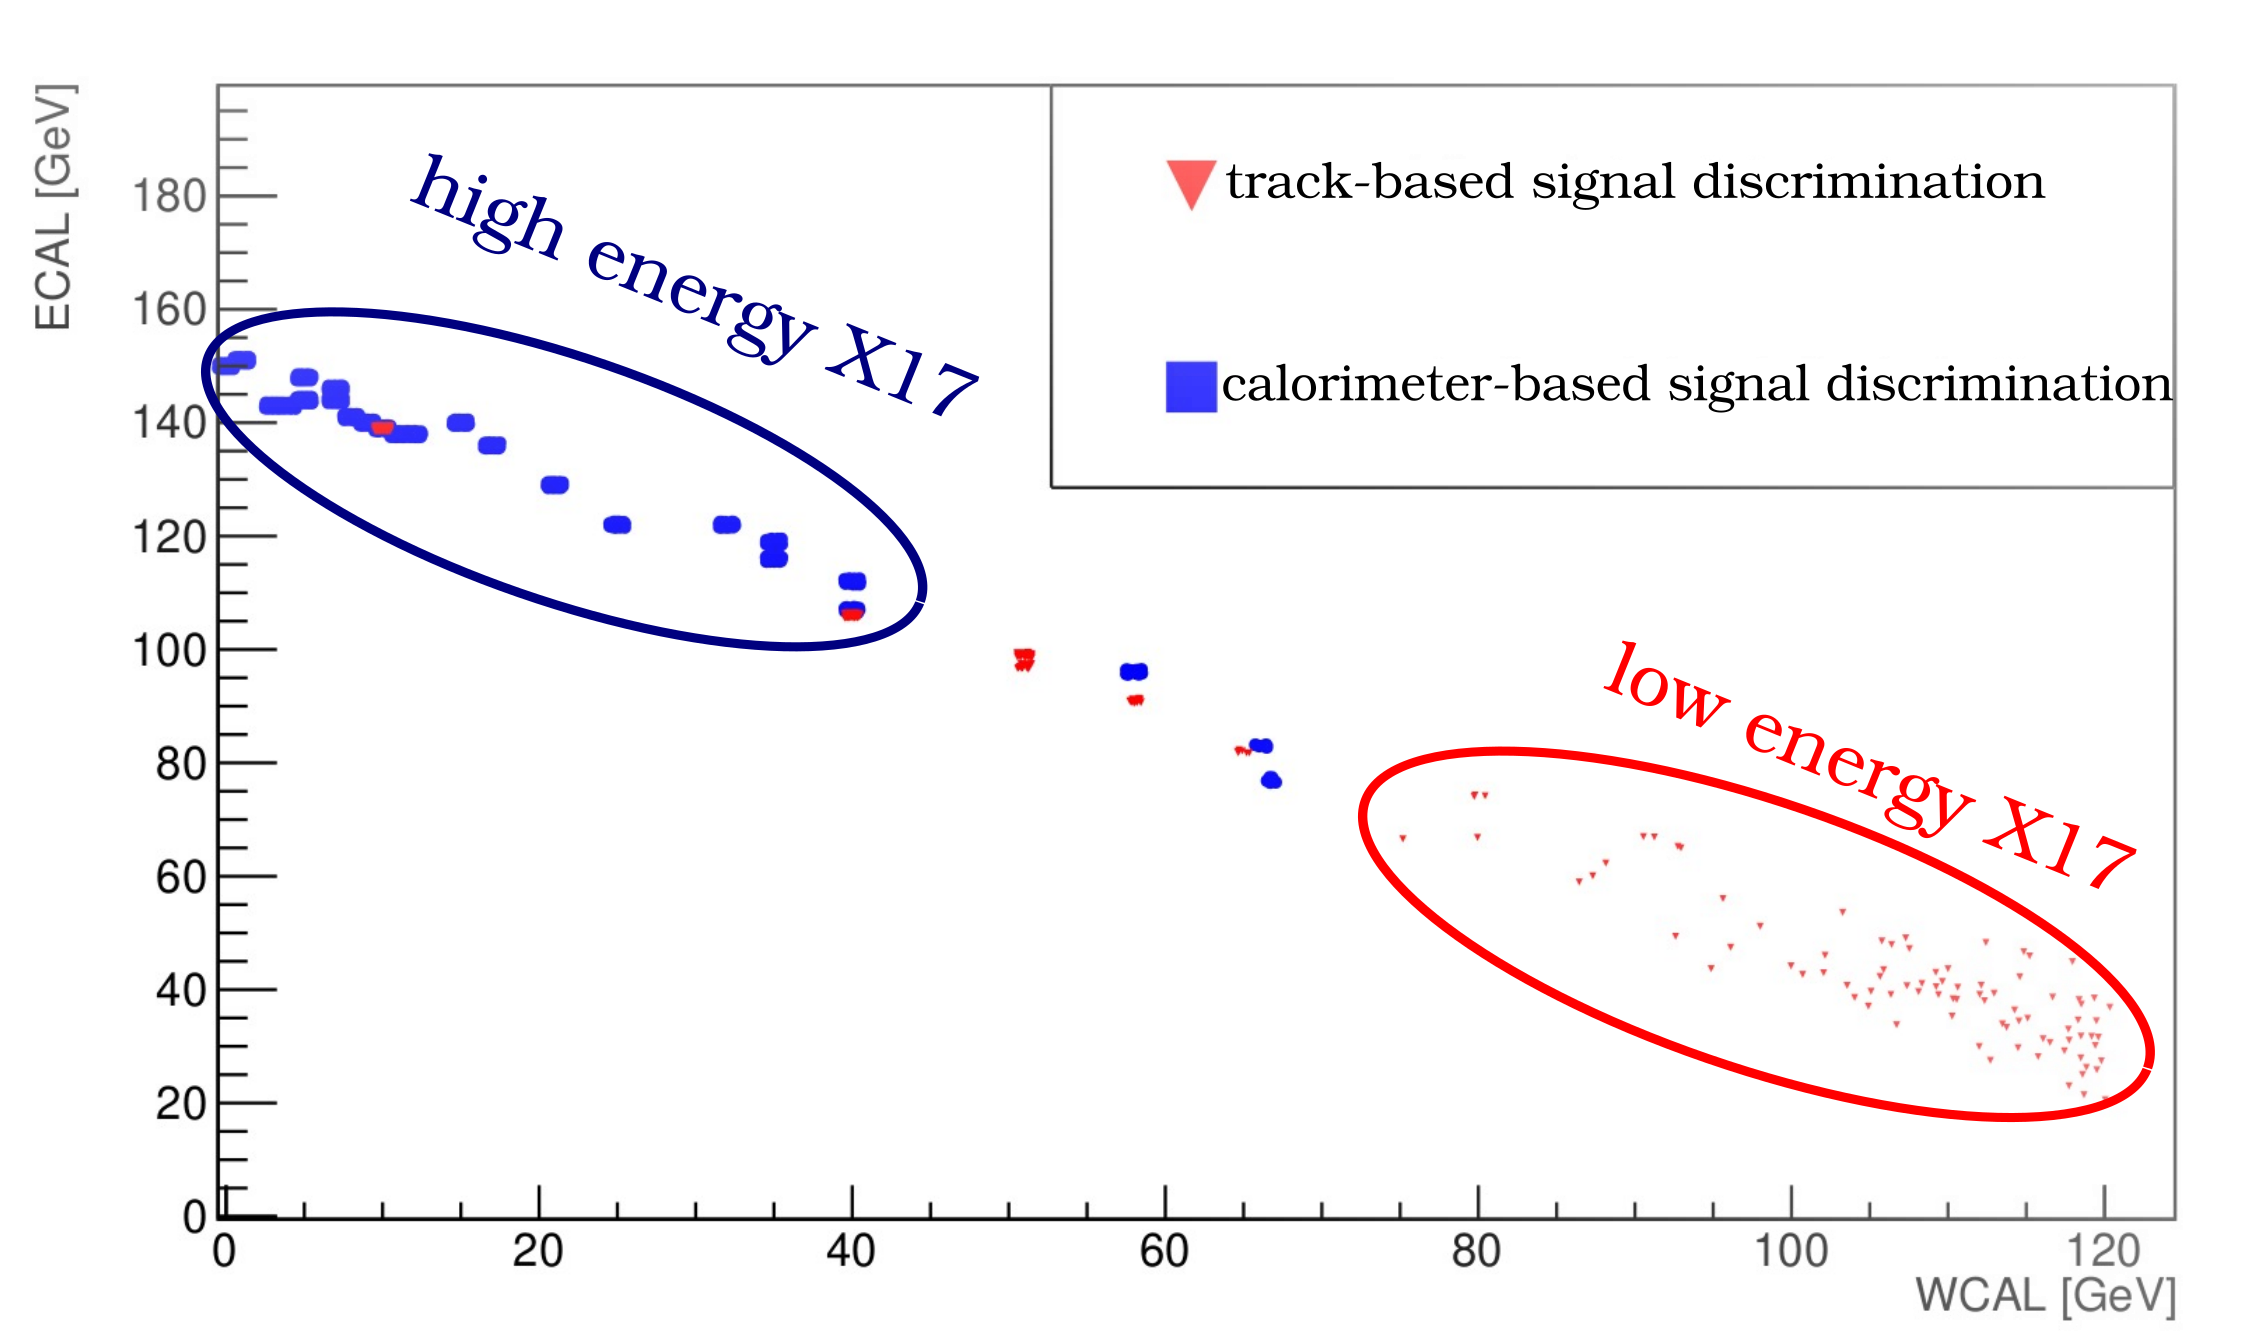
\includegraphics[width=\textwidth]{\pdirthree/X17-separation-v2.png}
  \caption[Comparison of selected $\DM$ events between the calorimeter and tracking analysis]{$\DM$ simulated in the visible mode 2018 setup. Two different cuts are used to discriminate between two $\DM$ topologies. The first one is based on angle and vertex position reconstructed using 4 GEM stations installed in the decay volume. It is very efficient on the $\DM$ produced at low energy (red triangle). The second one relies on the Veto placed at the end of the dump and is more efficient for the high-energy population (blue square).}
  \label{fig:combined-analysis}
\end{figure}

\begin{table}[h!]
  \centering
  \begin{tabular}{|llr|}
    \hline
    M$_{A'}$ [MeV]& $\epsilon$ & N$^{new}_{A'}$ / N$^{old}_{A'}$ \\    
    \hline
    5    & 0.004    & 1   \\    
    1    & 0.0015   & 1   \\    
    1    & 0.003    & 1   \\    
    16.7 & 0.0001   & 1.22\\
    16.7 & 0.00018  & 1.2 \\    
    16.7 & 0.000316 & 1.2 \\
    16.7 & 0.0006   & 1.01\\
    16.7 & 0.0007   & 1   \\
    22   & 0.000316 & 1.22\\
    \hline    
  \end{tabular}
  \caption[ratio between signal events observed in tracker-analysis compared to calorimeter-only analysis]{N$^{new}_{A'}$ / N$^{old}_{A'}$ ratio between signal events observed in the new tracker-analysis compared to calorimetry analysis. The new analysis uses GEM tracking detectors information if the energy detected by the downstream ECAL is below 75 $\gev$.}
  \label{tab:dm:efftable}
\end{table}

\subsubsection{$\gamma + Z \rightarrow \mu^+ \mu^-$ events in the visible mode analysis using trackers}
\label{ch3:sec:vis-mode-tracking-dimuon}

To validate the MC simulation and the tracking procedure required for this analysis, a pure sample of events containing the rare QED interaction $\emu$ has been studied. The double tracks expected in the decay volume from $\emu$ are used to test the reliability of the tracking procedure in the setup. In the MC, the tracks are prepared following the procedure described in Sec.\ref{ch3:sec:geant4-digitization}. The true MC hit information is convoluted with the GEM detector response. These tracks are then fed to the same reconstruction algorithm used for the data.

The reconstruction chain works as follows:
\begin{enumerate}
\item Track candidates are defined by grouping hits where the angle between first and second GEM pairs is smaller than 9 $\mrad$.
\item Those candidates are reconstructed using a Kalman filter implemented with the Genfit library \cite{genfit} (see Appendix.\ref{appD:sec:kalman-filter}).
\item Vertex candidates are generated by grouping track pairs with no common hits.
\item The exact position of the vertex is obtained by back-propagating the tracks at their point of minimum distance. Only vertices with a distance below 3 $\mmi$ are considered for the analysis.
\end{enumerate}

\begin{figure}[tbh!]
  \begin{center}
    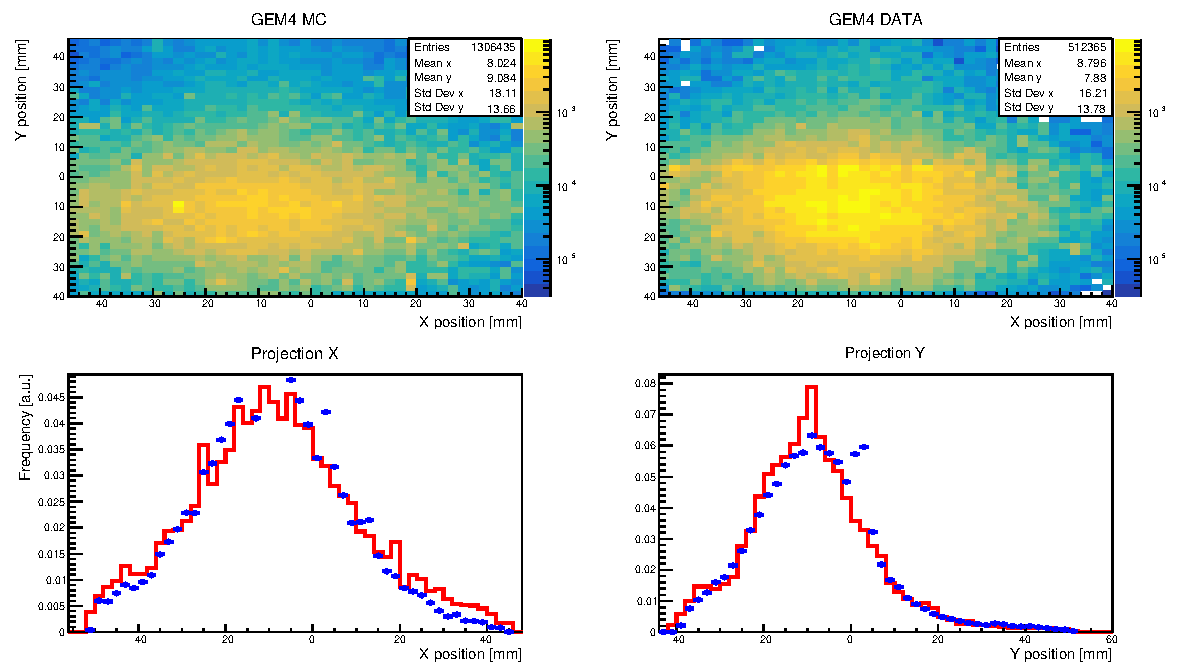
\includegraphics[width=\textwidth]{\pdirthree/GEM4_rel.pdf}
  \end{center}
  \caption[Hit position of $\emu$ in GEM MC-DATA]{Hit position recorded in last GEM before ECAL for MC simulated (Red curve) and data (Blue dots) $\emu$ events.}
  \label{fig:dimuon:gemspectra}
\end{figure}
  

A dimuon sample was selected using all events collected during the visible mode 2018 run. The $\emu$ events leave a double-MIP signature in each HCAL module, thus a cut 2 GeV$<$ E$_{hcal} <$ 6.35 GeV is applied for the selection. The beam quality was improved by requiring a reconstructed momentum in the range between 140 and 160 GeV. Since the physical trigger is used during the data taking (see Sec.\ref{ch2:sec:detectors-trigger}), an additional cut $E_{WCAL} < 90$ GeV is applied to consider only such events in both simulation and data. This cut also selects a sample with kinematics closer to the one expected from a $\DM$ candidate. This improves the comparison with the MC for our search. The energy in scintillator counters also needs to be compatible with a $\mu^+ \mu^-$ in the decay volume: energy deposited of at least 1 MIP is required in the scintillator (S4) downstream the WCAL and at least 1.8 MIP in the Veto behind the ECAL. 
The less stringent cut on S4 is justified by its limited transverse dimension which makes it not suitable for precise energy measurement.

A dimuon contribution is also expected from the hadron contamination. The physical trigger employed in the experiment further increases such contribution, as the requirement of low energy deposit in the WCAL bias the beam composition to particles with high penetration power. To solve this issue, a cut on the SRD detector and the WCAL pre-shower are used. These cuts are expected to reject hadrons and muons at a level of $\lesssim10^{-5}$.

To cross-check that the contamination is correctly removed, an independent method based on the beam profile shape is used. It significantly differs between electrons and hadrons as the H4 beamline is tuned for selecting electrons in our search. Both profiles are recovered from the data using a calibration run of electron/hadron respectively. Using a  $\chi^2$-test the ratio between the two is estimated by mixing the two templates until the best agreement with the measured beam profile is reached. The result is summarized in Fig.\ref{fig:dimuon:profile}: the beam profile of dimuon-selection events is compared before and after the SRD criteria are applied. The fit shows a contamination of roughly 50\% in the original sample. After the cut, the beam profile converges to the templates obtained in the $e^-$ calibration runs.

\begin{figure}[tbh!]
  \centering
    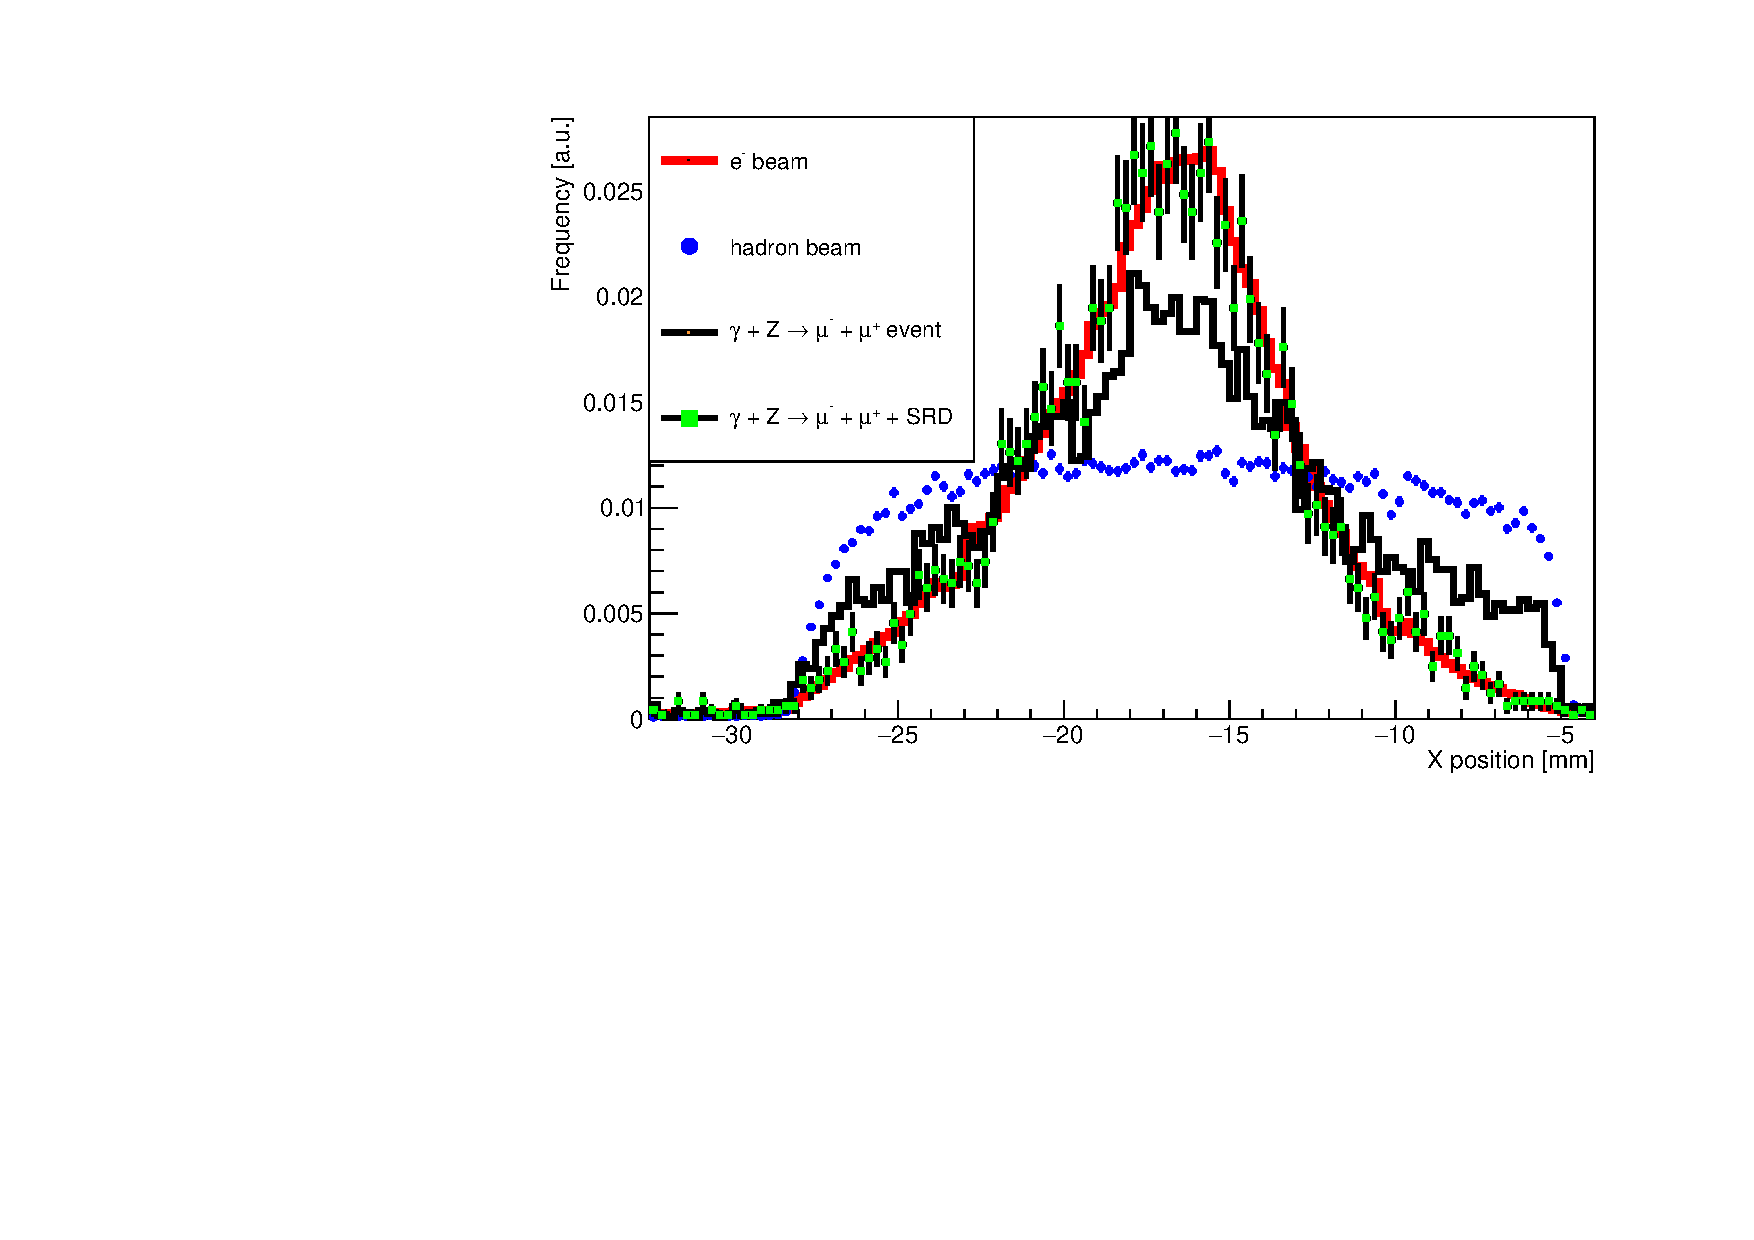
\includegraphics[width=\textwidth]{\pdirthree/beamspot.pdf}
  \caption[Beam profile with different cuts]{Beam profile recorded by the first Micromegas module upstream for hadron calibration run (blue dots), electron calibration run (red line), events selected with dimuons cuts from data collected with the physical trigger (black line), and those same events after applying SRD cut(green square). Fits using the templates obtained from the calibration run show a level of contamination of $\sim$50\% in the dimuon sample. The contamination is completely removed after the SRD selection.}
  \label{fig:dimuon:profile}
\end{figure}

\subsubsection{Signal yield correction}
\label{ch3:sec:dimuons-sig-corr}

To show that there are no significant differences in the tracking procedure in simulation and data the energy deposited in the WCAL was used as a figure of merit. After the vertex reconstruction selection, both distributions should still agree.
Following the procedure described above, vertex candidates are selected for the comparison. As the interaction $\emu$ will be produced inside the WCAL, only those vertices compatible with this assumption are selected for the comparison. In practice, a vertex is accepted if its position lies within 3$\sigma$ of the expected WCAL position, where $\sigma$ was fitted using a Gaussian from the distribution of $\mu^- \mu^+$ pairs selected from the simulation. After the selection criteria, the energy deposited in the WCAL is compared between simulation and data for each event left (see Fig.\ref{fig:dimuon_en}). The energy deposit for data and simulation is in excellent agreement, proving that the tracking cuts do not bias the original sample. Small disagreements in the order of 5\%-7\% are used to correct the signal yield using the procedure described in Sec.\ref{ch3:sec:dimuons}.

\begin{figure}[tbh!]
  \centering
    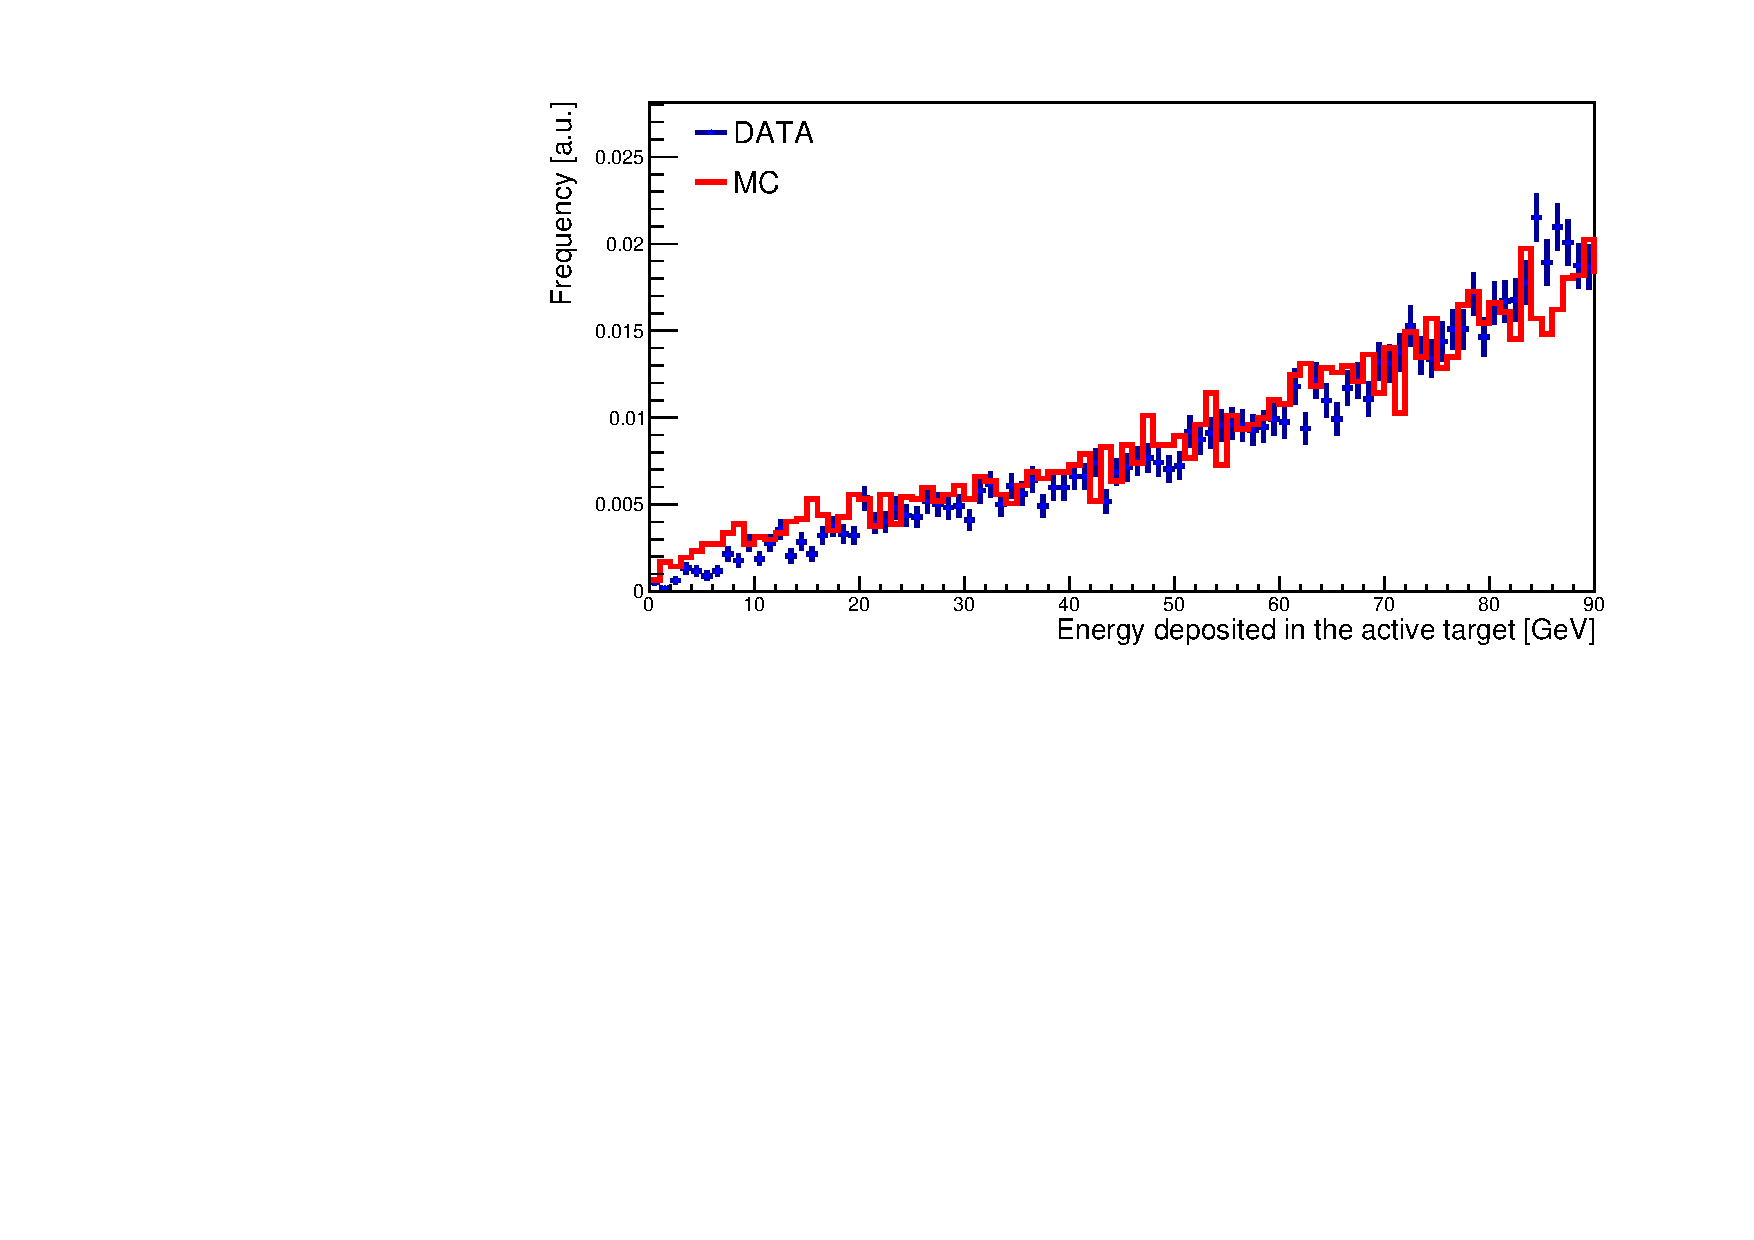
\includegraphics[width=\textwidth]{\pdirthree/dimuon_en.pdf}
  \caption[$\emu$ MC-DATA comparison in visible mode]{Energy deposit in the active dump (WCAL) after all selection criteria are applied in $\emu$ events. Data are drawn with blue dots, simulation is plotted with a red line.}
  \label{fig:dimuon_en}
\end{figure}

Lower efficiency is observed in the data compared to the Monte Carlo after applying the selection. The reasons for this are inefficiency of the GEM modules, fail of clusterization in some events, and differences in the tracking procedure due to the simplifications used in the MC. The cuts applied to the sample are divided into four steps. First, at least two hits per GEM are required in the decay volume as a minimal condition for tracking. After that, events with a GEM module recording more than 5 hits are rejected as incompatible with a single $\emu$ vertex. The MC predicts 68\% of $\mu^+ \mu^-$ pairs after these two cuts. This low acceptance is caused by the GEMs position optimized to resolve very close hits from the decay of $\DM$. These selection criteria do not depend on the track-fitting procedure but instead rely on the clusterization performed and the tracker's efficiency. Tracking procedure is then applied to the events that survived the two first requirements. The reconstructed vertex position is required to be compatible with a vertex inside the dump. The number of events surviving the last requirement is slightly smaller in the data. 
The disagreement between the ratio of good vertices reconstructed inside the decay volume is $<$1\%. A total factor of 0.77 is estimated as the ratio between data and MC. This factor is used to correct the 2018 signal yield. A summary of the efficiency can be found in Table \ref{tab:dimuon:efficiencies}.

\begin{center}
\begin{table}
  %\centering
  \begin{tabular}{|l|c|c|c|}
    \hline
    cut & efficiency MC & efficiency Data & MC / DATA \\
    \hline
    \multicolumn{4}{|l|}{\textbf{Hit}}\\
    \hline
    hits per GEM $\geq$ 2 & 0.68$\pm$0.1 & 0.58$\pm$0.1 & 0.85$\pm$0.1 \\
    hits per GEM $\leq$ 5 & 0.68$\pm$0.1 & 0.55$\pm$0.1 & 0.80$\pm$0.1 \\
    \hline
    \multicolumn{4}{|l|}{\textbf{Tracking}}\\    
    \hline
    Vertex distance $\leq$ 3 $\mmi$ & 0.63$\pm$0.1 & 0.49$\pm$0.1 & 0.77$\pm$0.1  \\
    Vertex in decay volume & 0.62$\pm$0.1 & 0.48$\pm$0.1 & \textbf{0.77$\pm$0.1}\\
    \hline
    
  \end{tabular}
  \caption[MC/DATA for the tracking procedure and vertex reconstruction]{Cut efficiency based on tracking criteria for a clean sample of simulated $\emu$ and dimuon selected from 2018 data. The efficiencies presented in the table are cumulative, with the first cut applied being the one in the first row. The first two cuts are based exclusively on information coming from the single GEM modules. The last two are based on the tracking procedure.}
  \label{tab:dimuon:efficiencies}
\end{table}
\end{center}

\subsection{Background}
\label{ch3:sec:bkg:vis}

Since the energy deposited in the two calorimeters (WCAL and ECAL) should be equal to the incoming primary energy, particles escaping the setup in the transverse direction are no longer a source of background as in the invisible mode. Because of the large distance between the WCAL and ECAL\footnote{7.5 \si{\meter} in the 2018 setup, 4.2 \si{\meter} in the 2017 setup}, such event is actually frequently observed. The background, on the other hand, can be caused by particles able to punch-through the first target without leaving any energy deposit in the W2 counter and then leave a pure electromagnetic signature in the ECAL downstream. Because of the different lengths of the setup and the addition of a vacuum tube (see Fig.\ref{fig:setup-vis-2018}), the background calculated for 2017 and 2018 differs significantly. The suppression depends on the exact source of background considered, but it can amount up to one order of magnitude \cite{Banerjee:2019hmi}. However, the background conditions do not differ significantly between the classical calorimetry approach and the new analysis using the trackers. The values expected for both cases are reported in Table \ref{tab:vis-bkg}.


\subsubsection{Hadronic background}
\label{ch3:sec:bkg:vis:hadr}

Starting from the most simple scenario, punch-through of $\pi^-$ can be background if no energy is deposited in the W2 counter, an energy $> 2\emip$ is measured in S$_4$, and the pion is stopped in the ECAL. The product of these probabilities was conservatively estimated to be $< 10^{-12}$ when SRD and HCAL suppression is included.

Inelastic scattering in the WCAL, for example in the form of

\begin{equation}
  \label{eq:vis-int-neutral}
  \pi^- + p \rightarrow (\geq 1)\pi^0 + (neutrals)
\end{equation}
can produce particles that travel through the W2 undetected. The background was estimated using an extrapolation of the charge-exchange cross-section, measured for different nuclei, after taking into account the SRD suppression. In the tracking-analysis, inelastic scattering in the WCAL produces a large occupancy in the decay volume that can potentially create vertex candidates. Such events are suppressed by the hadron rejection selection criteria applied downstream outlined in Sec.\ref{ch3:sec:selection-criteria-vis}. Furthermore, events able to mimic the pure electromagnetic signal of the decay $\DM \rightarrow e^+ e^-$ are often accompanied by a large transversal spread and are thus rejected by the requirement of energy conservation at a level of $\lesssim 10^{-5}$. This estimate was obtained in a $\pi^-$ simulation by integrating the events in the signal region with two tracks in the decay volume without applying any hadron rejection criteria. Such an event should also pass the independent selection criteria applied upstream, namely large energy deposited in the SRD and WCAL pre-shower. In a $10^7$ EOT sample, there was no event with such signature even after removing the HCAL and VETO from the selection criteria.

To estimate the background for a larger number of EOT, the $\ks$ decay was used as a benchmark process, as its short decay length is expected to be compatible with the $\DM$ ones. The energy spectrum of $\ks$ was simulated using an exponential distribution with an energy cut-off of 18 GeV, as below this energy has a negligible probability to decay outside the dump. To estimate the number of $\ks$ in the sample, events with a punch-through neutral were selected by applying all selection criteria to the control sample but changing the requirement for $S_4$ to $E_{S_4} < 0.5 \emip$. The distribution of these events is shown in Fig.\ref{fig:w-e-vis}. Here we label signal-like events that passed all selection criteria in the control sample. One such event was recorded in 2017, well outside the signal region. In 2018 the number of neutral was reduced by a factor 2-3, and no signal-like events were observed. These data were used to estimate the ratio between neutral and signal-like events using the MC-simulation of $\ks$. This resulted in an estimate of 0.06 events for the 2017 data and 0.005 events for 2018 data. The statistical fluctuation of the data dominates the error for this estimate.

To estimate the background for the tracking analysis, tracking-criteria were applied over the $\ks$ MC-sample. Rejection of $10^{-2}$ can be conservatively achieved using the opening angle of the reconstructed vertex as a discriminator. This estimate however mostly depends on the main hadronic decay channel $\ks \rightarrow \pi^- + \pi^+$ which is further suppressed downstream by the hadron suppression cuts such as no energy deposited in the HCAL and the VETO. The decay channel $K^0_S \rightarrow \pi^0 + \pi^0$ has on the other hand a small chance to leave a signature in the GEM modules as no charged particle is typically emitted. Signal-like events can be produced either by the conversion of a photon from the $\pi^0 \rightarrow \gamma \gamma$ decay into a $\pair$ pair or in the decay chain $\ks \rightarrow \pi^0 + \pi^0 (\pi^0 \rightarrow \gamma + e^- + e^+$). This last channel is however suppressed by its low branching ratio $\Gamma_i$/$\Gamma \approx $1\% \cite{review-particle-physics}. A dedicated simulation performed with a biased branching ratio shows that the rejection for this channel is further improved to $\lesssim 10^{-3}$ since the large emission angle of a three-body decay is significantly different from the one expected in the $\xdecay$ decay. A conservative rejection of $\lesssim 10^{-5}$ is reached accounting for both suppression factors. If we add the suppression factor coming from the angle using the trackers to what was computed for the calorimeter-analysis, one can conservatively estimate the background contribution from $\ks$ to be at a level of $<0.001$.


\begin{figure}[bth!]
  \centering
  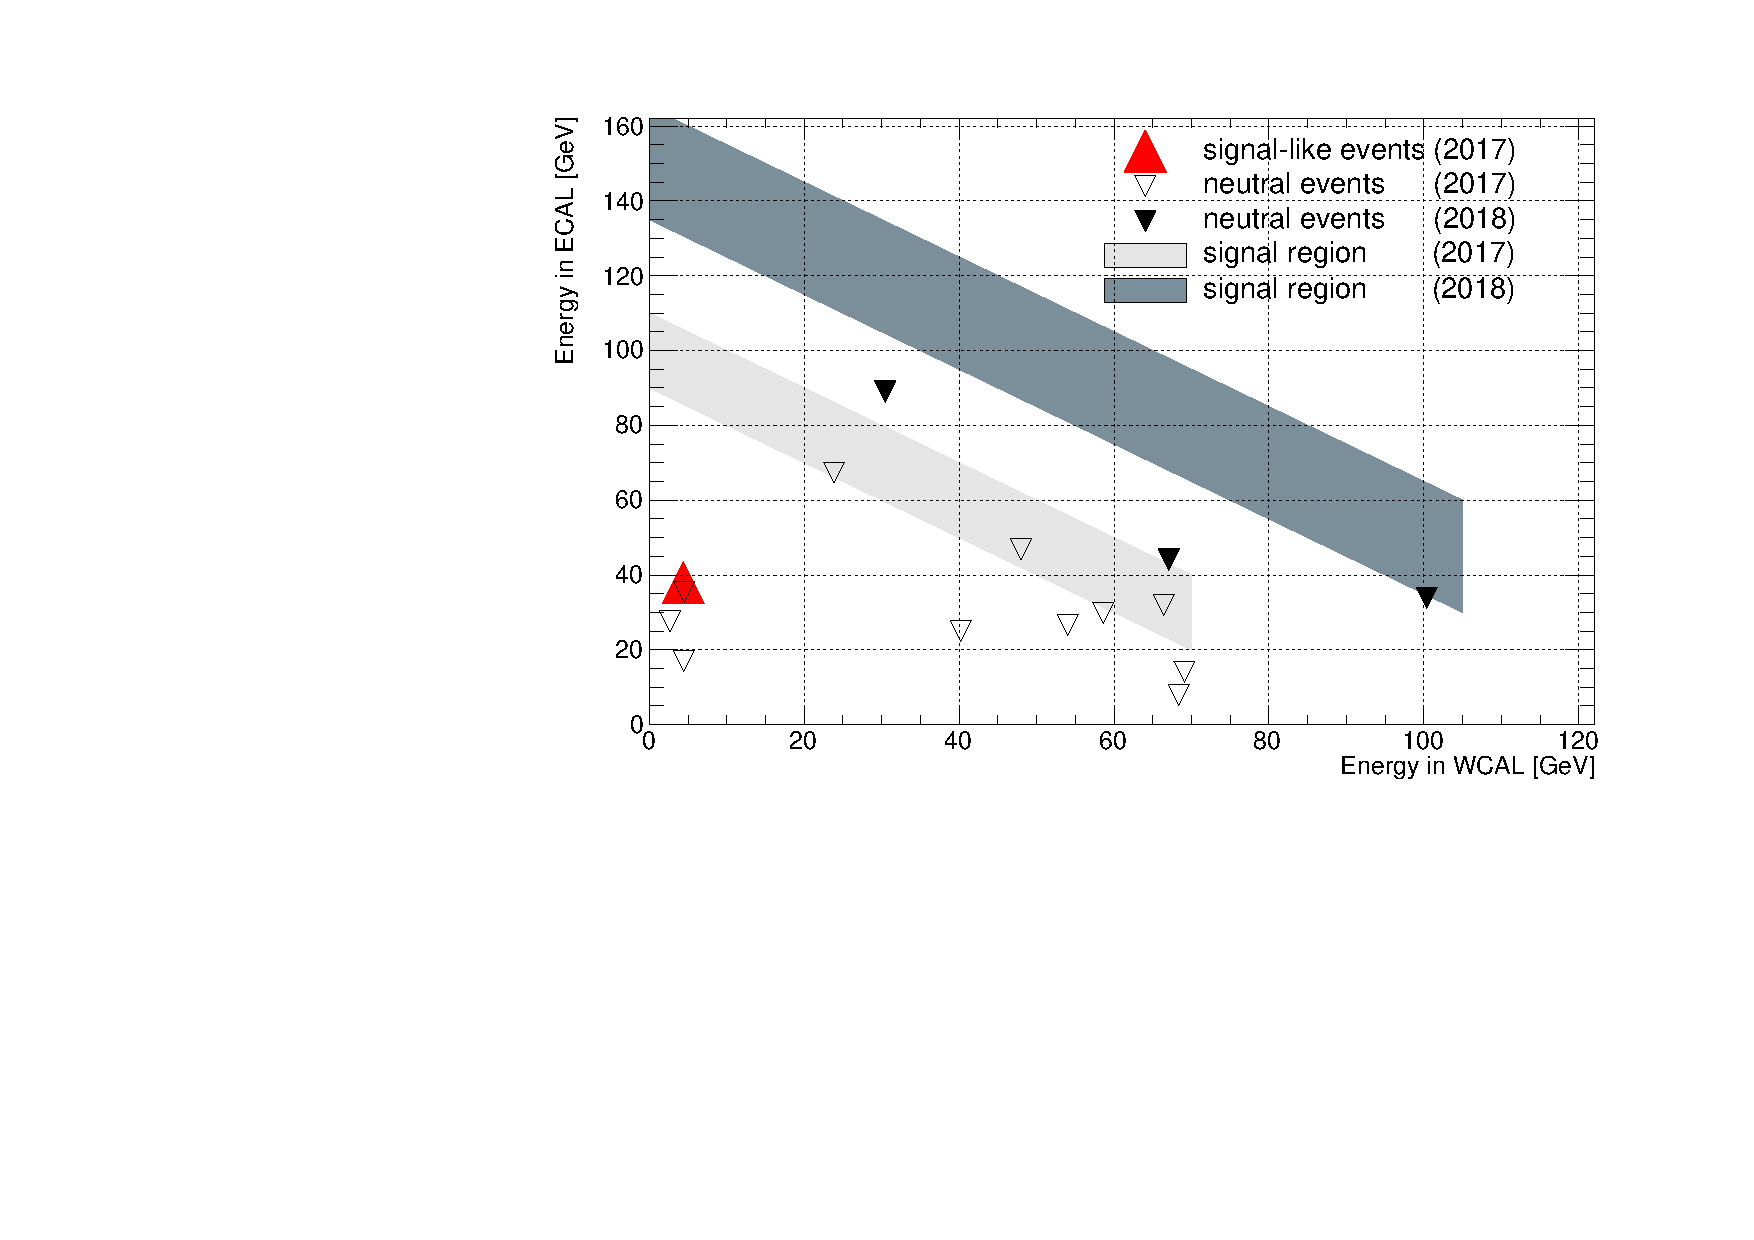
\includegraphics[width=\textwidth]{\pdirthree/w-e-neutrals.pdf}
  \caption[neutral events in visible mode]{Distribution of selected signal-like events in the $\ehcalplane$ plane for 2017 and 2018 data. Neutral events are shown as hollow (2017) and full (2018) triangles. The two shadowed bands represent the signal box region for the two different runs. A single signal-like event detected during the 2017 run not falling into the signal region is shown with a red triangle \cite{Banerjee:2019hmi}.}
  \label{fig:w-e-vis}
\end{figure}

\subsubsection{Muonic background}
\label{ch3:sec:bkg:vis:muon}

Background coming from $\mu^-$ primaries is very suppressed in the visible mode. It is dominated by the probability of $\mu^-$ punch-through that leaves most of its energy inside the ECAL. This is similar to the $\pi^-$ case, with the difference that its probability to leak in the signal region is lower due to the absence of strong interaction for $\mu^-$. The background can be conservatively estimated to be $<10^{-14}$.

\subsubsection{Electronic background}
\label{ch3:sec:bkg:vis:elec}

The main contribution of the background from $e^-$ primary is the punch-through of high-energetic $\gamma$ that converts on the last tile of the WCAL producing an $\ee$ pair. Since it depends on the longitudinal fluctuation of the em-shower, it is hard to predict using MC-simulations alone. To estimate such contribution for $\sim10^{11}$ EOT a data-driven method is used instead. A sample of 3$\cdot 10^9$ EOT was considered, roughly corresponding to $\sim$10\% of the data collected in 2018. Events in the signal region with $E_{ECAL} < 105$ GeV were selected with the requirement of at least two hits in each GEM module. Only one event with such property was found. An additional suppression of $10^{-3}$ is introduced by the tracking selection criteria (or the W2 cut for the calorimetry analysis). This put the background to a level $<10^{-13}$. The analysis of the full 2018 data is compatible with this estimate: a total of three events were found with 2 two hits in the GEM modules. For none of these events, it was possible to reconstruct a physical vertex, suggesting that these particles experienced large multiple-scattering inside the WCAL before reaching the GEMs.


\begin{table}[bth!]
  \centering
  \caption[Visible mode background]{Expected background for 5.5$\times$ $10^{10}$ EOT collected in 2017 \cite{Banerjee:2018vgk} and the 3.3$\times$ $10^{10}$ EOT collected in 2018 \cite{Banerjee:2019hmi}. The third column shows background for 2018 including the GEM trackers in the analysis.}
  \begin{tabular}{lrrr}
    \hline \hline
    Background source                           & $n_b$ (2017)      &  $n_b$ (2018)   & $n_b$ (2018, new analysis)\\
    \hline
    $\pi^-$ punch-through                        & 0.0015$\pm$0.0008 &  0.0007$\pm$0.0004   & 0.0007$\pm$0.0004   \\    
    $\ks \rightarrow \pi^0 \pi^0$                     & 0.06$\pm$0.03    & 0.005$\pm$0.003 &     $<$0.001\\
    $e^-$/hadron nuclear interaction  & 0.01$\pm$0.004    & 0.01$\pm$0.004  & 0.01$\pm$0.004\\    
    $\mu^-$ punch-through                        & $<0.001$ & $<0.001$ & $<0.001$       \\            
    $\pi^-$,$K^- \rightarrow e\nu$ $K_{4e}$              & $<$0.001 & $<0.001$ & $<0.001$\\
    $eZ \rightarrow e Z \mu^+\mu^-;\mu^{\pm}\rightarrow e^{\pm}\nu\bar{\nu}$ & $<$0.001 & $<0.001$ & $<0.001$\\
    punch-through $\gamma$ & $<$0.001 & $<$0.0005 & $<$0.001 \\
    \hline
    Total (conservatively)                      & 0.07 $\pm$ 0.04   & 0.006 $\pm$ 0.003  & 0.006 $\pm$ 0.003\\
    \hline \hline                       
  \end{tabular}
  \label{tab:vis-bkg}
\end{table}

%%% Local Variables:
%%% mode: latex
%%% TeX-master: "../PhDthesis"
%%% End:
